\documentclass{article}
\usepackage{blindtext}
\usepackage{titlesec}
\usepackage{listings}
\usepackage{geometry}
\usepackage{mathtools}
\usepackage[utf8]{inputenc}
\usepackage{siunitx}
\usepackage{soul}
\usepackage{enumitem}
\usepackage{graphicx}
\usepackage{float}
\usepackage{units}
\usepackage{amsfonts}
\usepackage{amsmath}
\usepackage{nth}
\usepackage{multirow}

\geometry{
 a4paper,
 total={170mm,257mm},
 left=20mm,
 top=20mm,
 }
 
\newcommand\tab[1][1cm]{\hspace*{#1}}
\setlength{\parindent}{0pt}

\title{Advanced Signal Processing}

\author{
  Pranav Malhotra, CID:\num{00823617}
}
\date{2nd February 2016}

\begin{document}

\begin{titlepage}
	\centering
	{\scshape\LARGE Imperial College London \par}
	\vspace{2cm}
	{\scshape\Large Advanced Signal Processing \par}
	\vspace{2.5cm}
	{\Large\itshape Pranav Malhotra, CID: 00823617 \par}
	\vfill
% Bottom of the page
	{\large \today\par}
\end{titlepage}

\tableofcontents
\newpage
\section{Random signals and stochastic processes}
\subsection{Statistical Estimation}
To explore random signals and stochastic processes, it is of great importance that we learn how to generate random signals. Below, is a plot of a vector that consists of a $1000$ samples, each of which is an independent realisations of the random variable $X\sim \mathcal{U}(0,1)$. The vector is first graphed using the {\tt plot} function, which returns a continuous-time description of the signal; it is formed by linear interpolation between the samples. If we wish to interpret the samples as a discrete-time signal, we use the {\tt stem} function.



\begin{figure}[H]
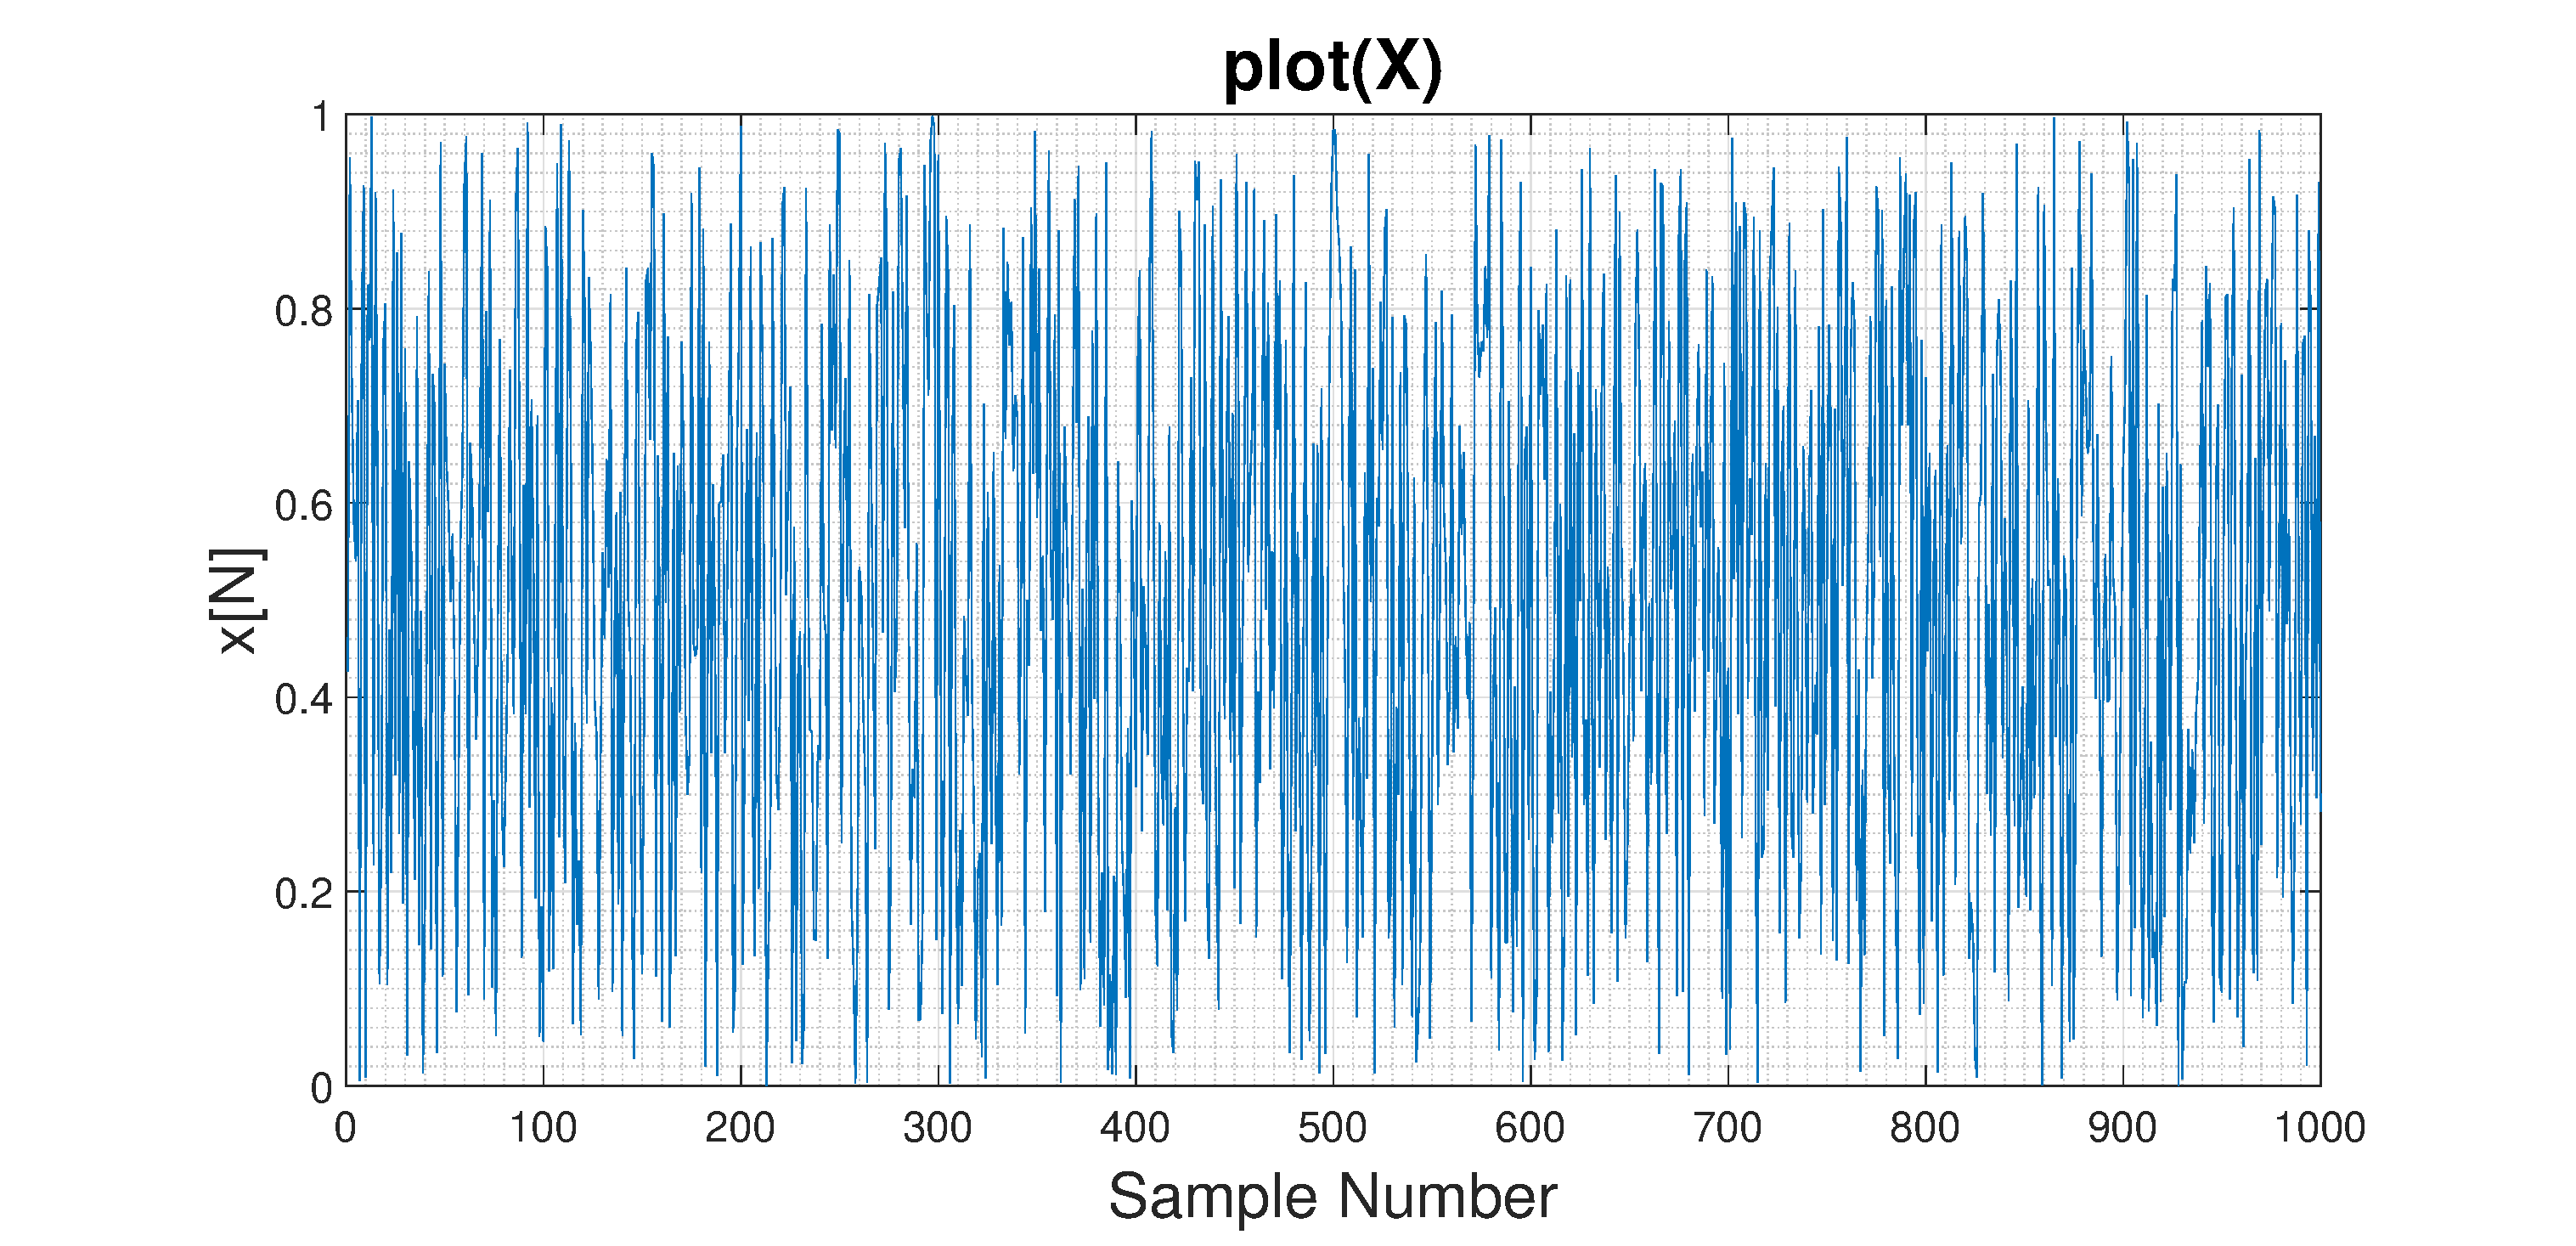
\includegraphics[width=0.49\textwidth]{plot_x}
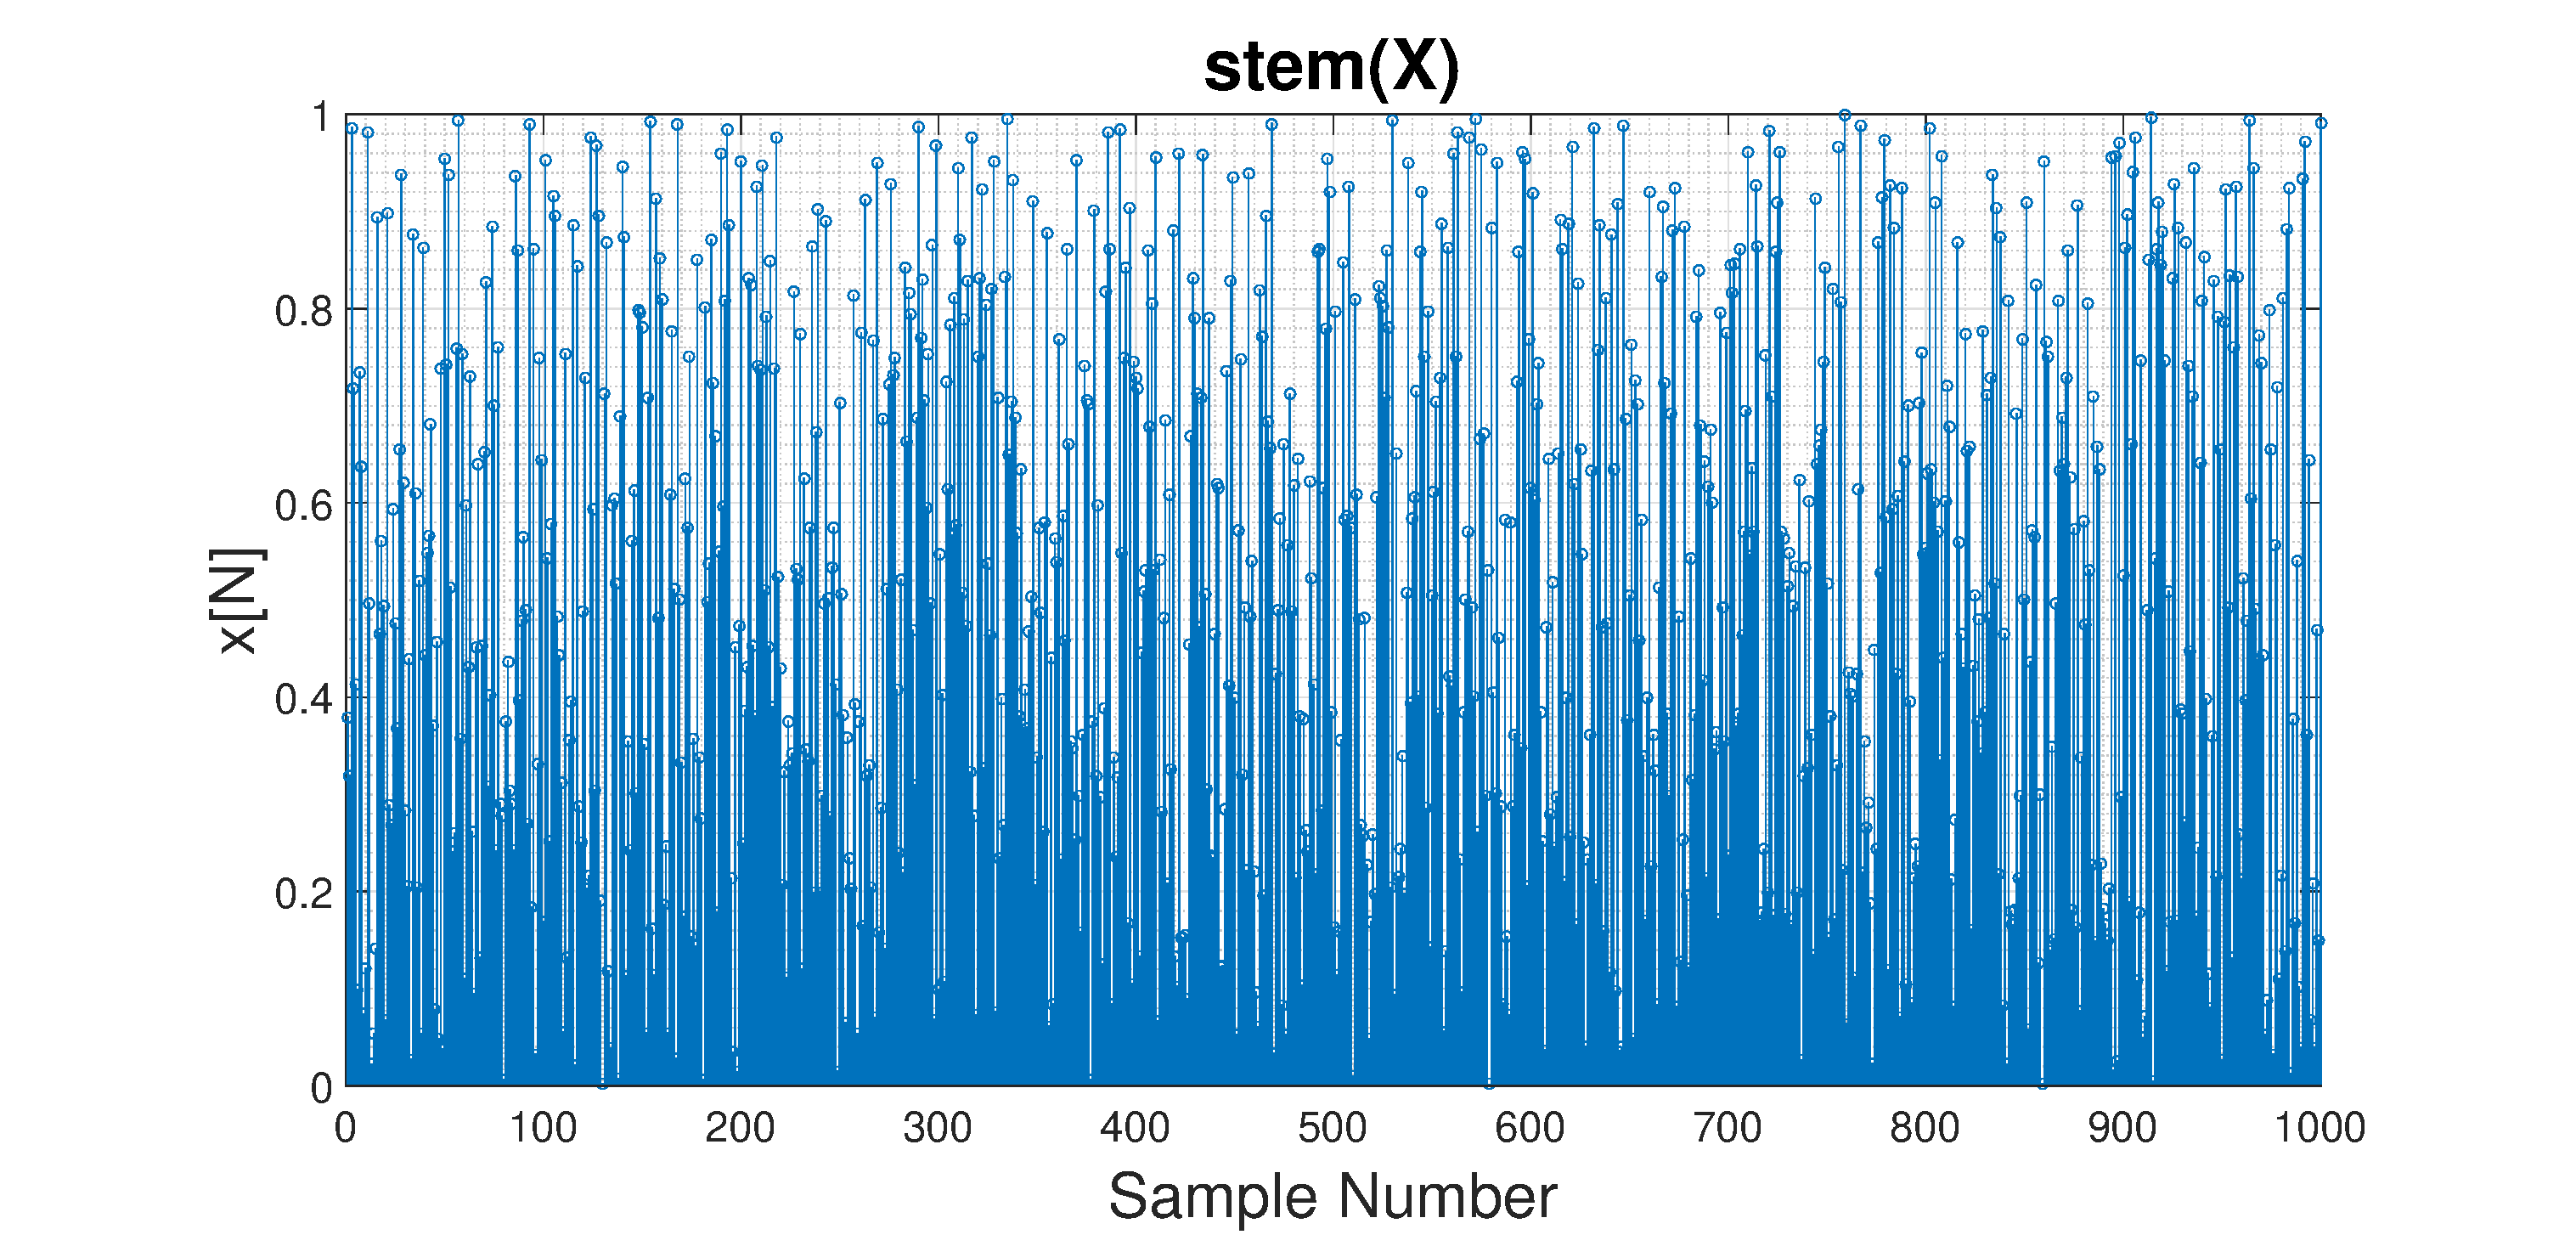
\includegraphics[width=0.49\textwidth]{stem_x}
\caption{Plot and stem of a $1000$ samples drawn from $X\sim \mathcal{U}(0,1)$}
\end{figure}

From the sequence, it is clear that there is some sort of uniformity although the samples are completely independent. This uniformity stems from the fact that the samples are independent realisations of the same random variable and thus the mean and variance of the signal is time-invariant.\\

1. To calculate the theoretical mean of the random variable $X\sim \mathcal{U}(0,1)$, the statistical expectation operator is employed.

\begin{equation}
    Theoretical \ Mean = \mathbb{E}\{X\} = \int_{-\infty}^{\infty} xf_{X}(x)dx = 0.5\nonumber
\end{equation}
In MATLAB, the {\tt mean} function returned a value of $0.4888$. The calculated sample mean, $\hat{m}$ is a function of the random samples; we can represent the sample mean as a random variable, $\hat{M}$ whose  distribution depends on the underlying distribution of the individual samples. The calculated sample mean, $\hat{m}$ is a single realisation the random variable $\hat{M}$. If the samples are drawn from a distribution with a mean, $\mu$ and a variance, $\sigma^{2}$, then the sample mean will have a mean, $\mu$ and a variance, $\nicefrac{\sigma^{2}}{N}$, where N is the number of samples. It is clear that the sample mean is an unbiased estimator of the theoretical mean and that its accuracy increases with the number of samples. Also, it is interesting to note that by the \textit{central limit theorem} (CLT), if a sufficiently large number of samples is used, the random variable $\hat{M}$ will follow a Gaussian distribution such that $\hat{M}\sim \mathcal{N}(\mu, \nicefrac{\sigma^{2}}{N})$.\\

2. To calculate the theoretical variance of the random variable $X\sim \mathcal{U}(0, 1)$, the statistical expectation operator is once again employed. The argument of the operator is slightly different.

\begin{equation}
    Theoretical \ Variance = \mathbb{E}\{(X-\mu)^{2}\} = \mathbb{E}\{X^{2}\} - \mathbb{E}\{X\}^{2} = \int_{-\infty}^{\infty} x^{2}f_{X}(x)dx - \mathbb{E}\{X\}^{2} = \frac{1}{12}\nonumber
\end{equation}

\begin{equation}
    Theoretical \ Standard \ Deviation, \ \sigma = \sqrt{\nicefrac{1}{12}} \approx 0.2887\nonumber
\end{equation}

In MATLAB, the {\tt std} function returned a value of $0.2832$. The calculated sample standard deviation, $\hat{\sigma}$ is also a function of the individual samples and thus the sample standard deviation can also be represented by a random variable. The calculations are, however a lot more involved that the calculations for the sample mean. It is important to note that the sample standard deviation is also an unbiased estimator of the theoretical variance. Just like the sample mean, the accuracy of the estimator increases with the number of samples.

\newpage
3. The sample mean and sample standard deviation are graphed for each member of the ensemble. The plots clearly show that the two estimators are both unbiased as the means and standard deviations hover around their theoretical values.  
\begin{figure}[H]
\includegraphics[width=0.49\textwidth]{sample_mean_vs_realisation_number_rand}
\includegraphics[width=0.49\textwidth]{sample_standard_deviation_vs_realisation_number_rand}
\caption{Sample mean and sample standard deviation for each member of the ensemble, samples considered are uniformly distributed}
\end{figure}

4. Estimating the \textit{probability density function} (PDF) is of great importance in statistical signal processing. The PDF underlying the random samples is estimated using the {\tt hist} function in MATLAB and is normalised using the {\tt trapz} function. To measure the performance of our PDF estimator, a reference line is included that marks the theoretical PDF of the uniform distribution.
\begin{figure}[H]
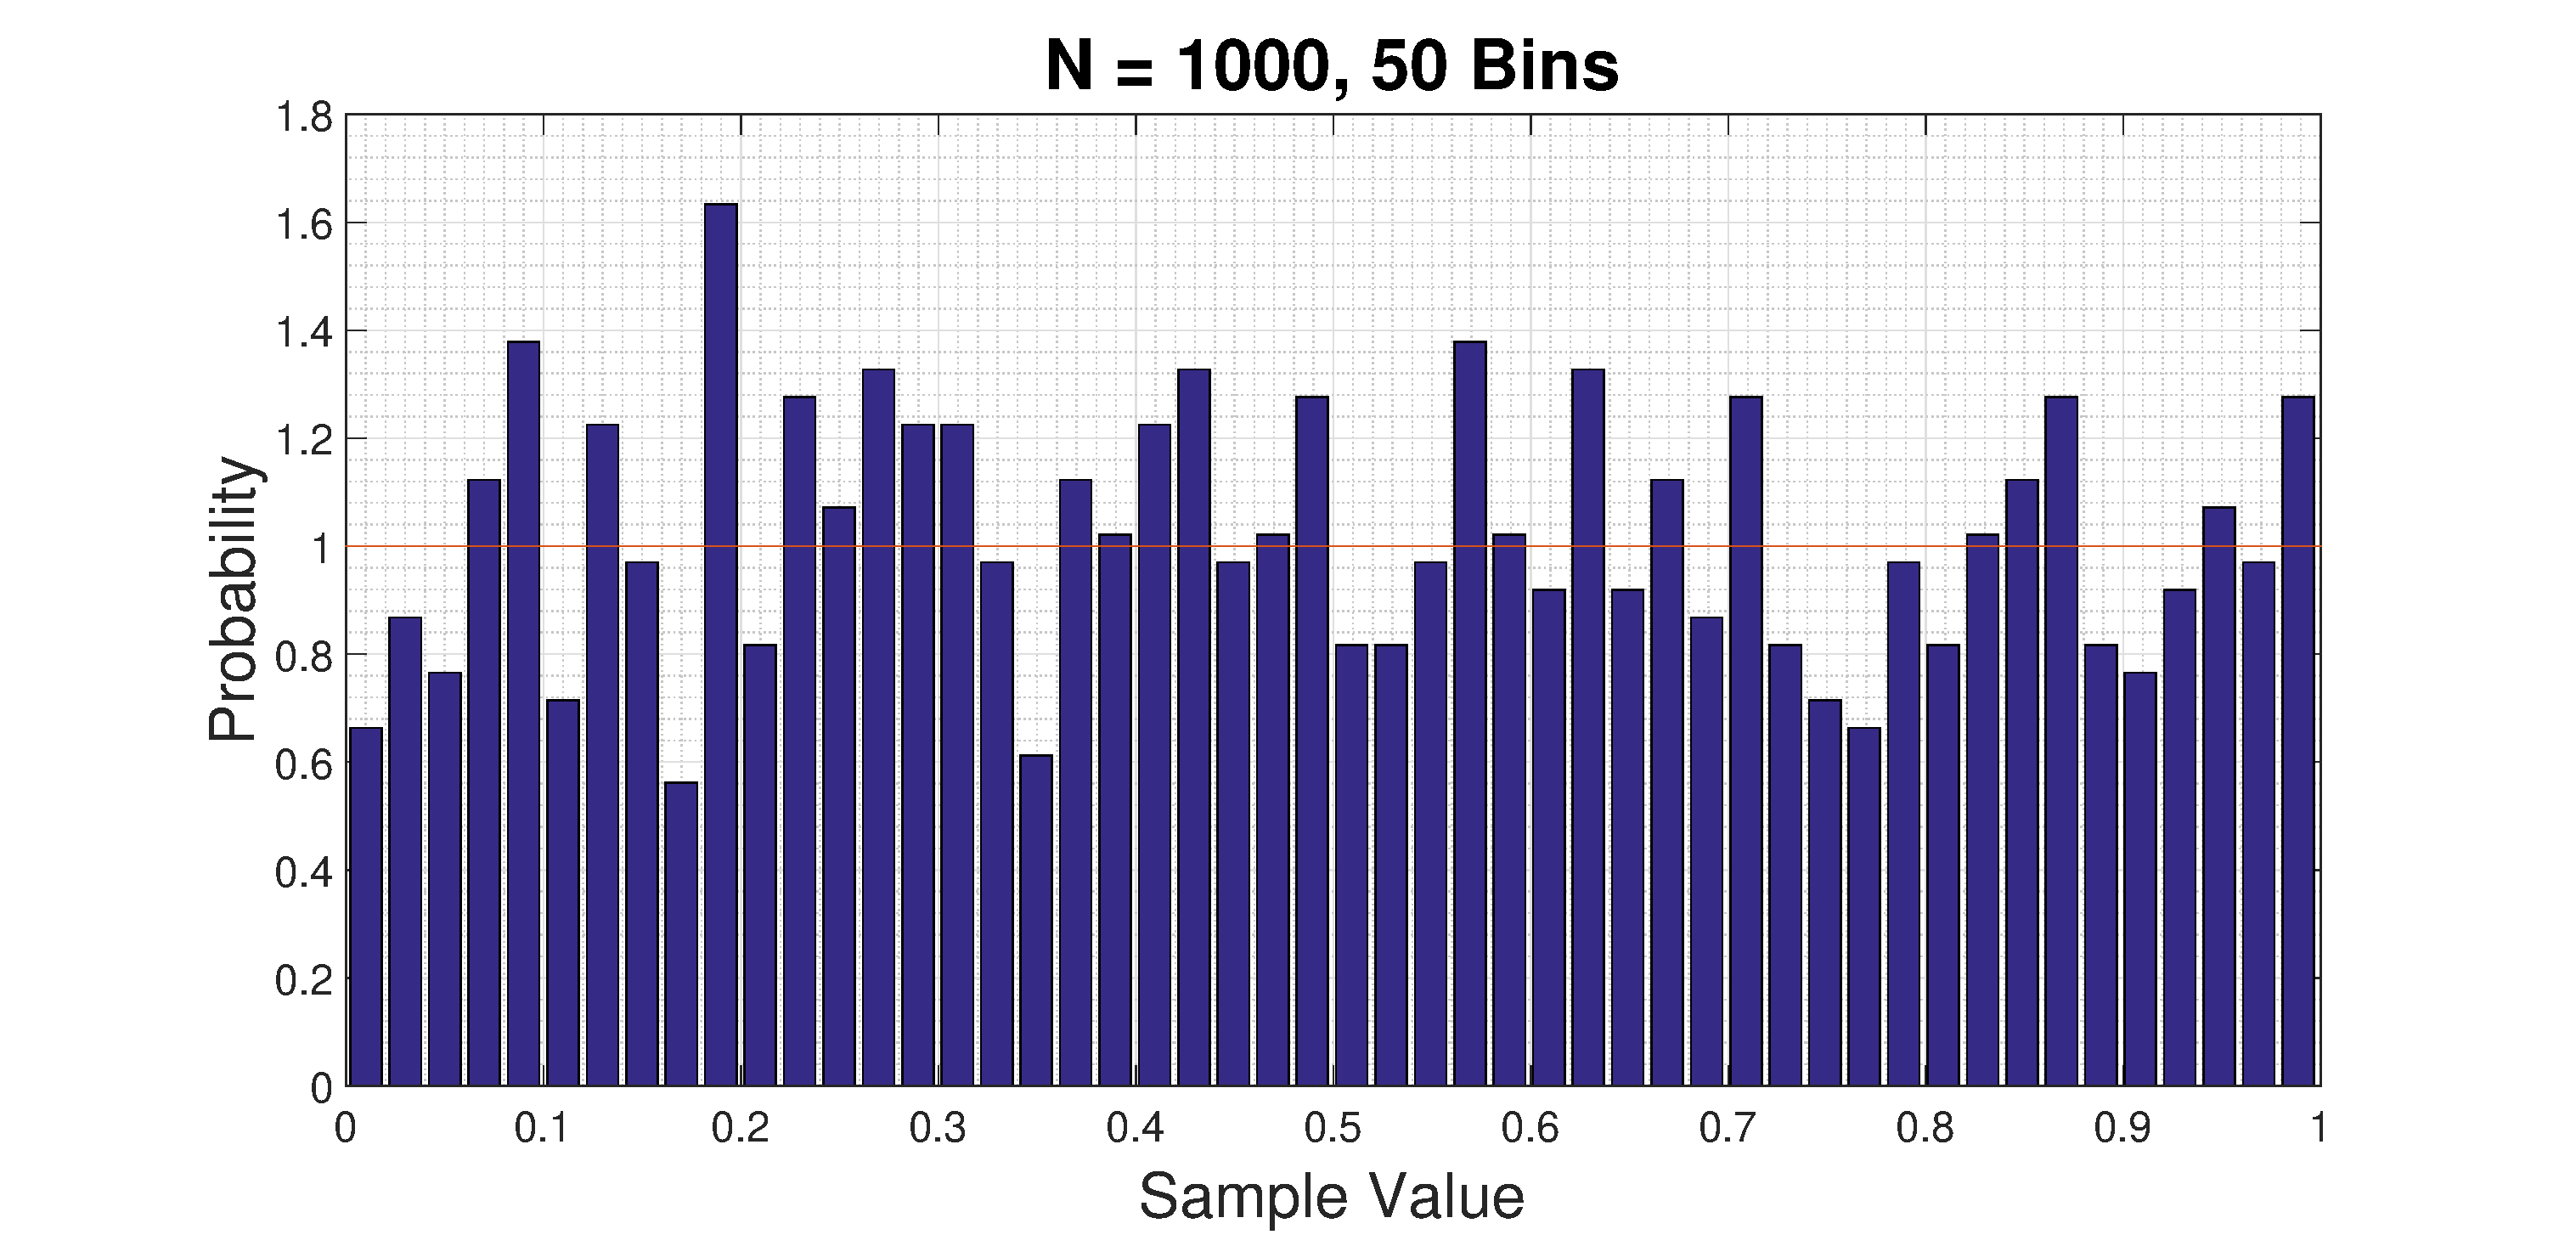
\includegraphics[width=0.49\textwidth]{N_1000_B_50_rand}
\includegraphics[width=0.49\textwidth]{N_1000_B_100_rand}
\caption{Approximate PDF of random samples drawn from $X\sim \mathcal{U}(0,1)$, small sample size}
\end{figure}

Increasing the bin size will result in better resolution of the estimated PDF, however arbitrarily increasing the bin size is not wise and will result in unclear results. Increasing the sample size significantly improves the estimate and the result approaches the theoretical PDF.

\begin{figure}[H]
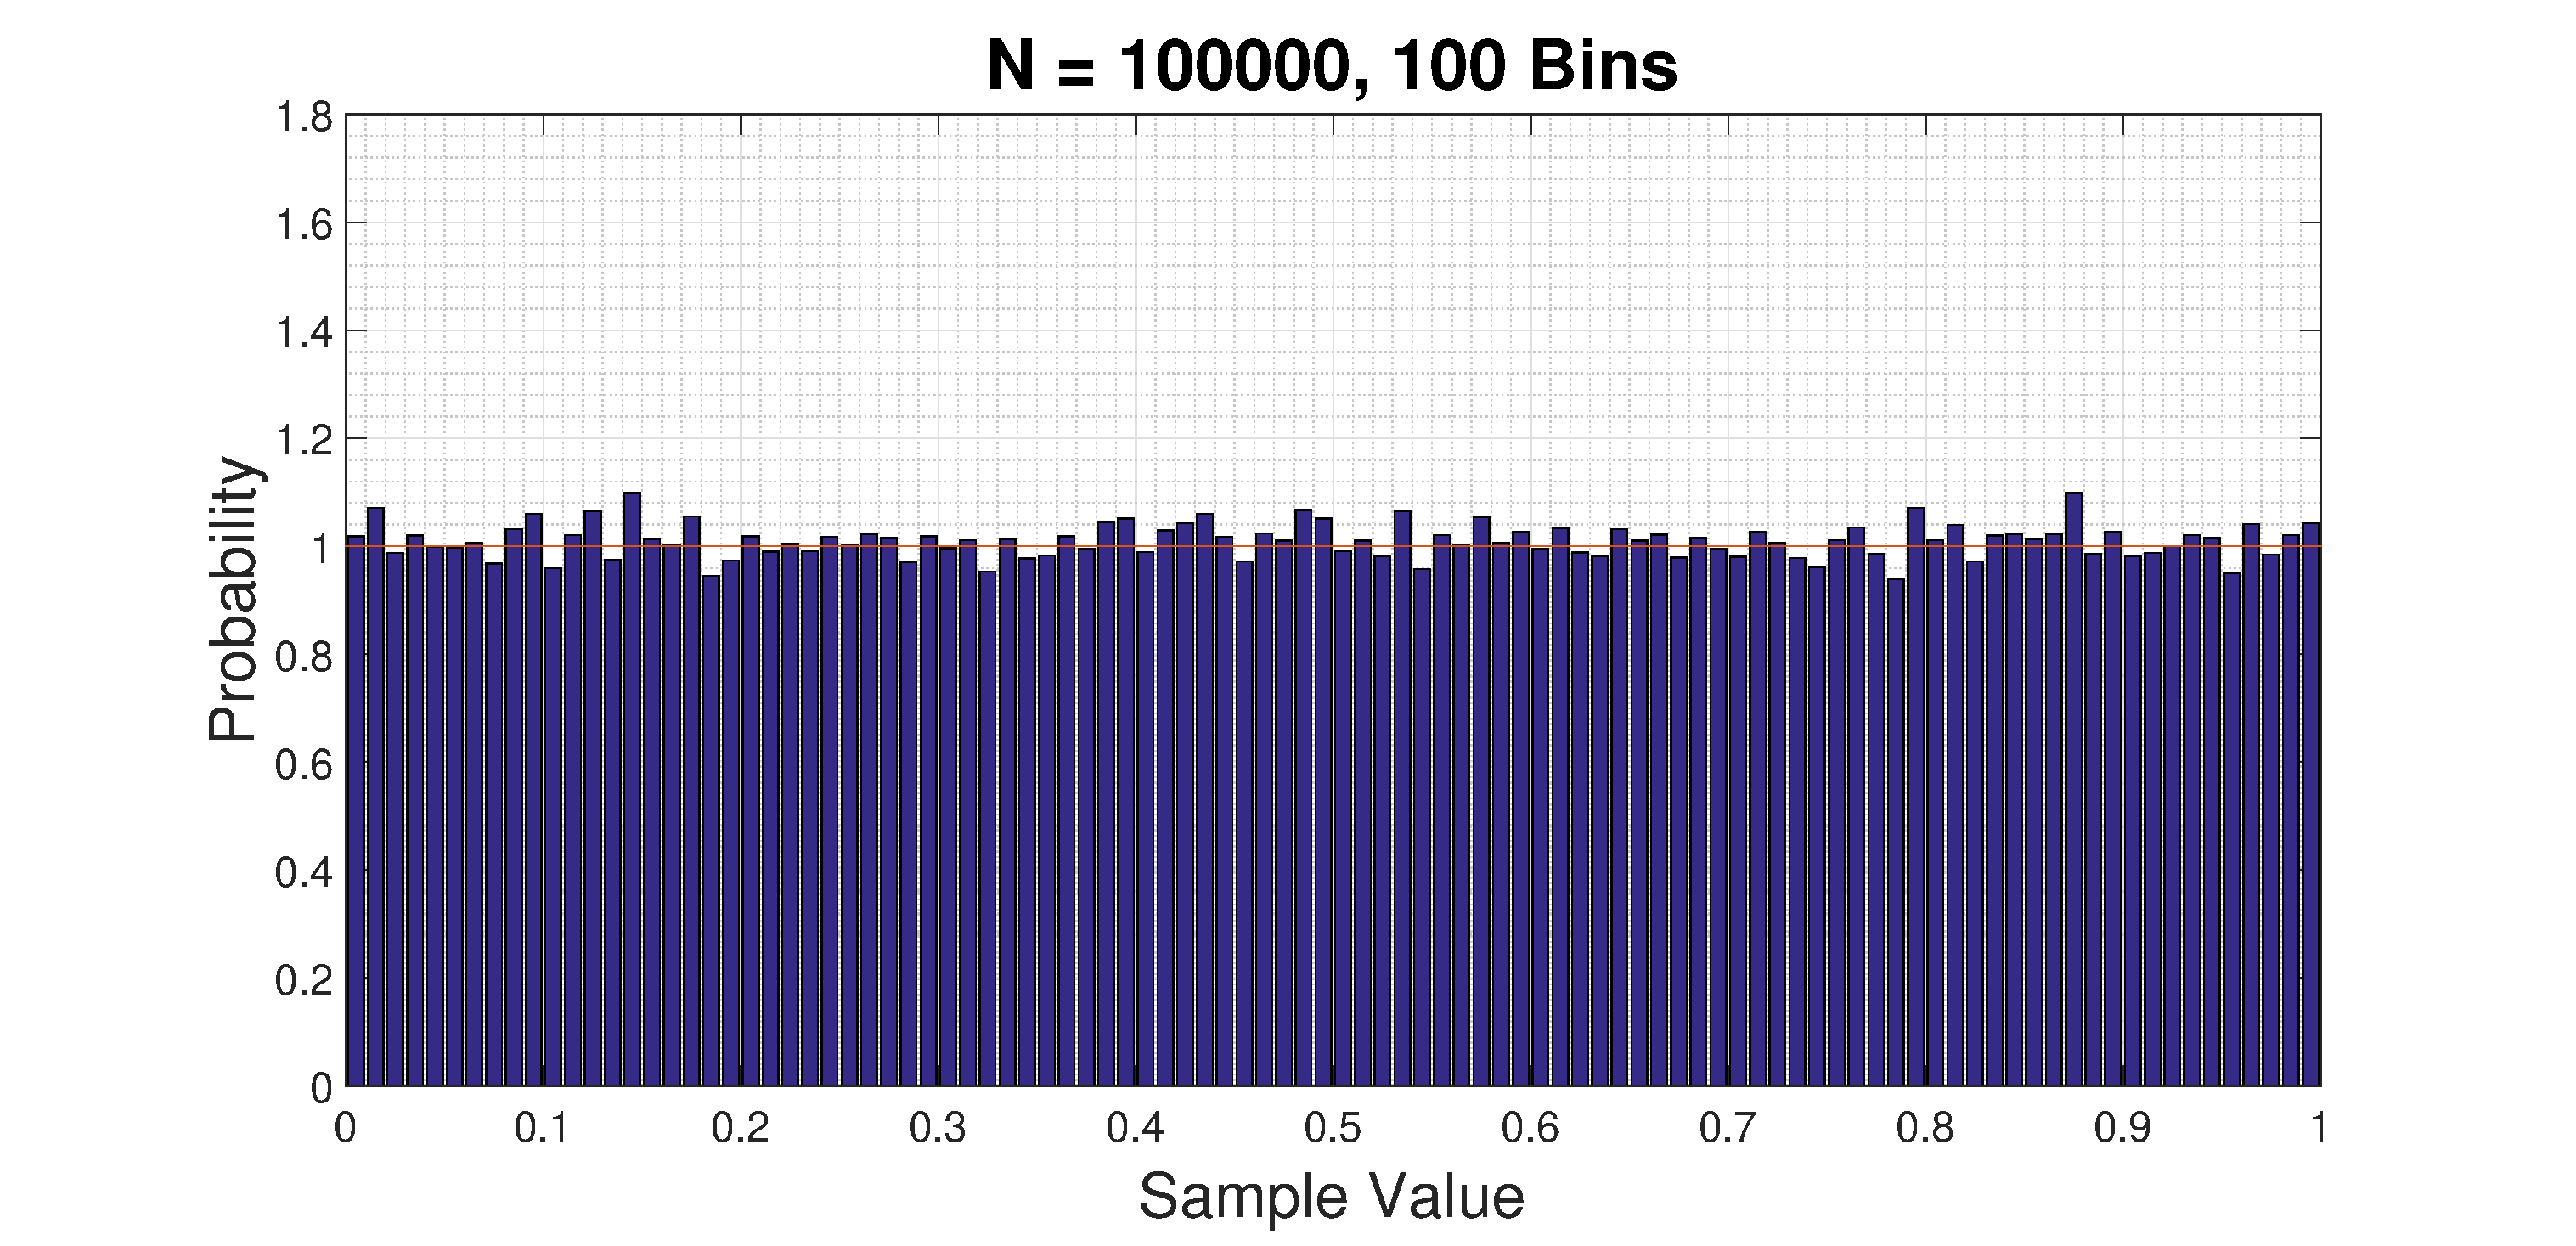
\includegraphics[width=0.49\textwidth]{N_100000_B_100_rand}
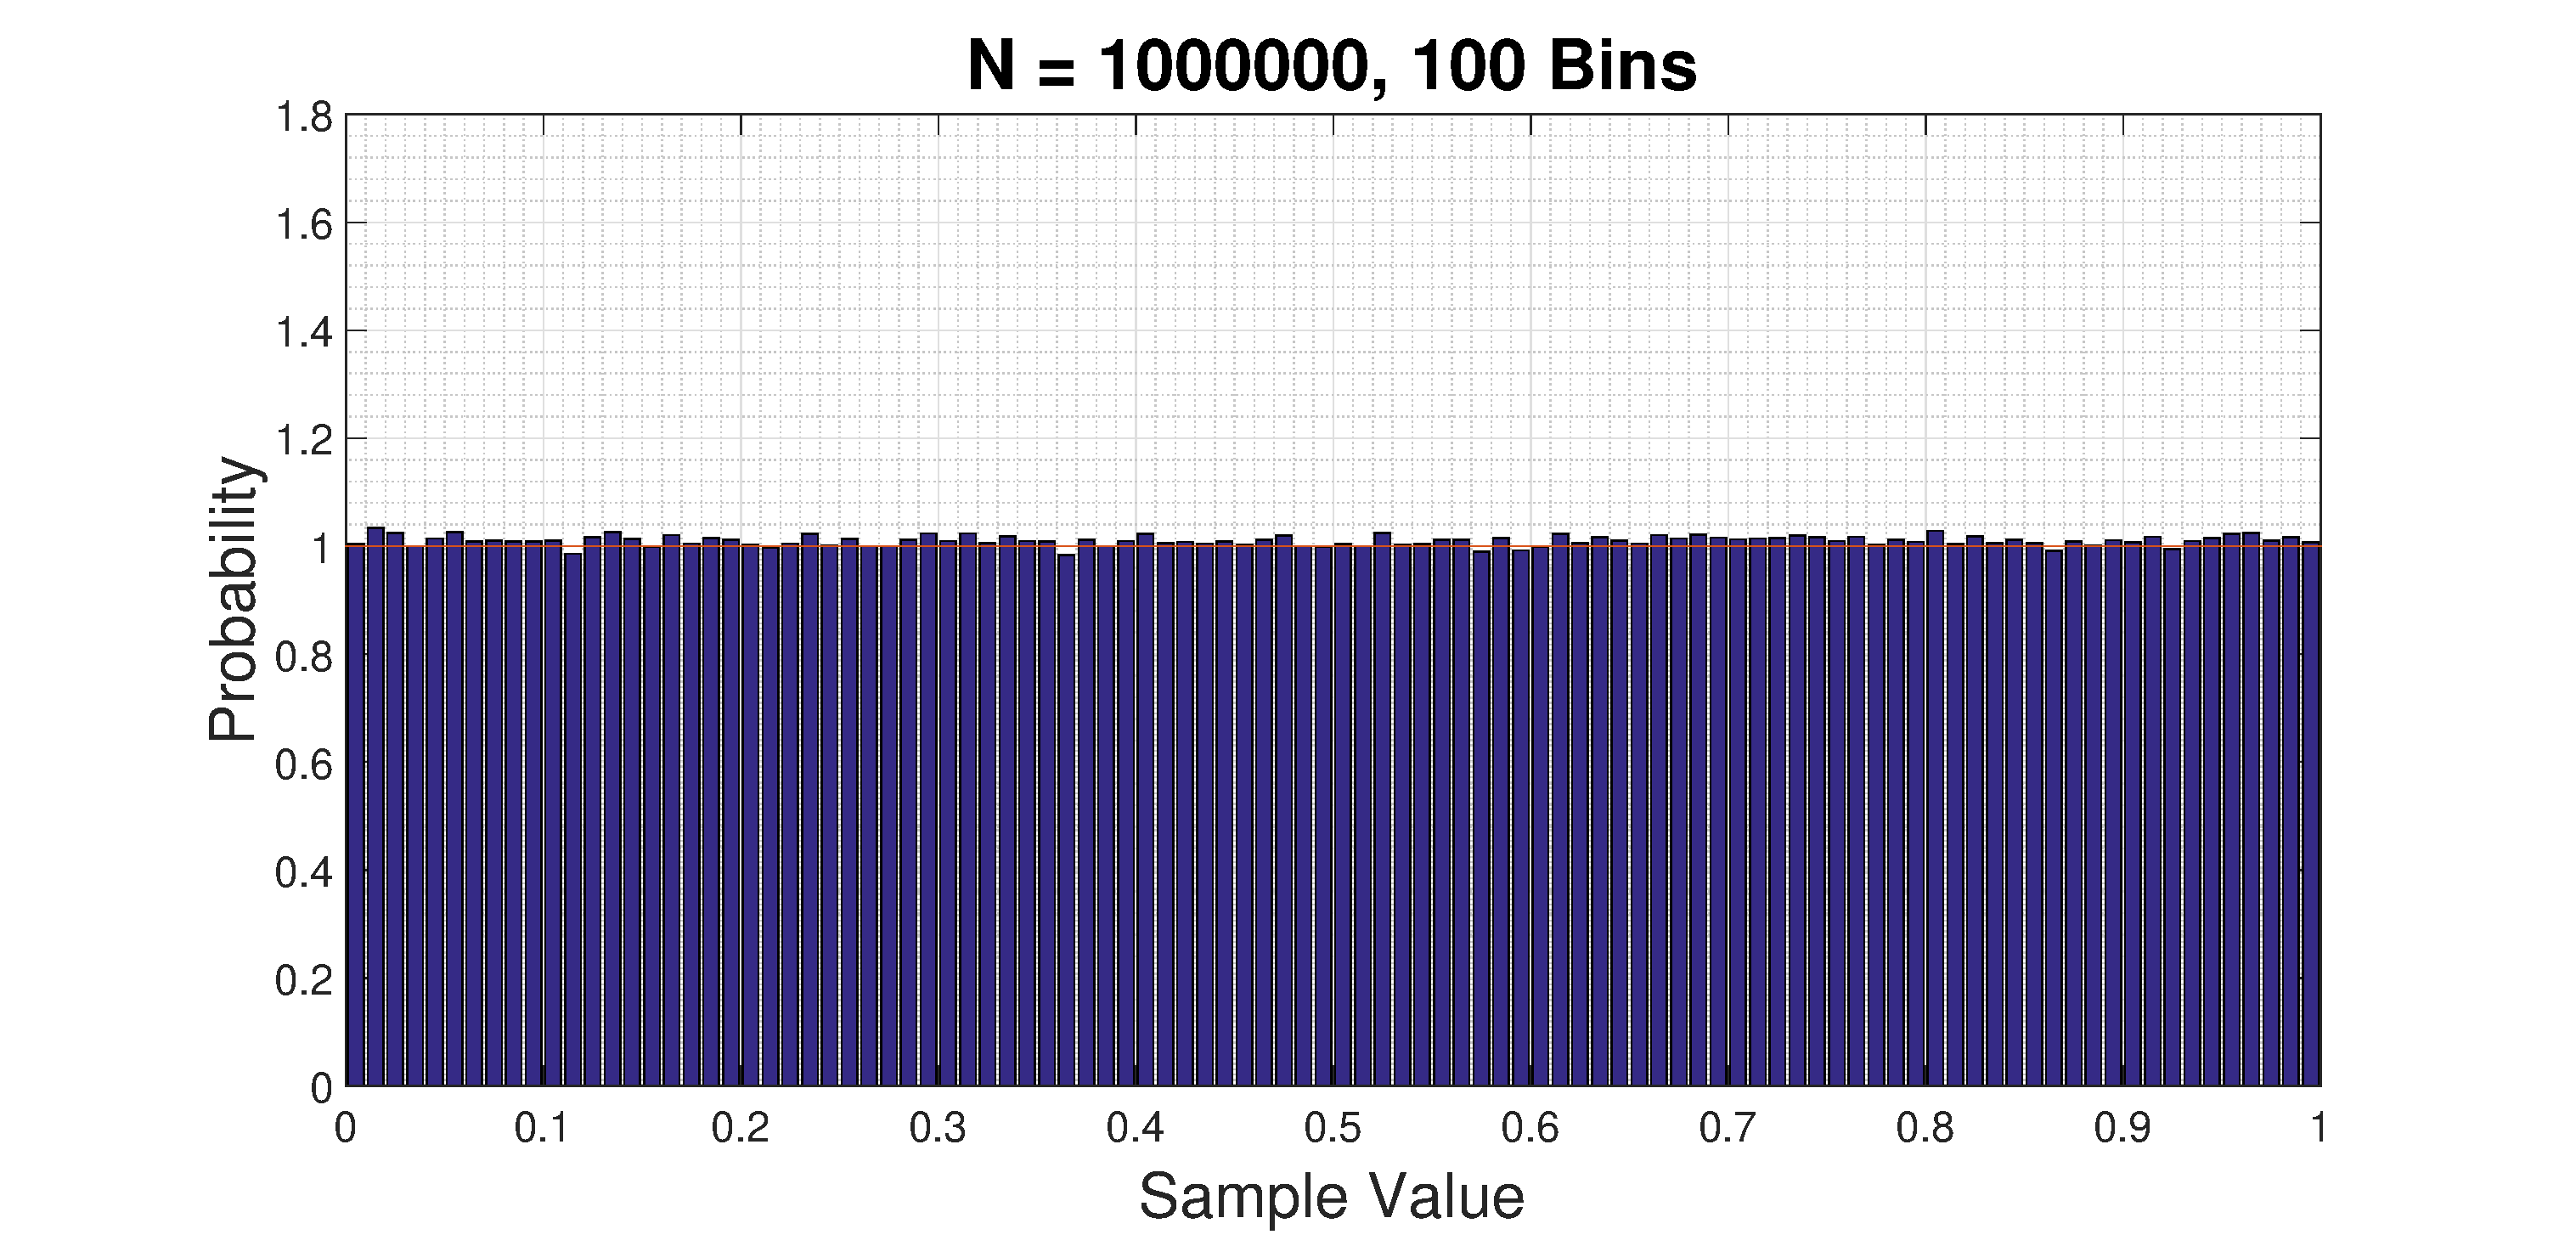
\includegraphics[width=0.49\textwidth]{N_1000000_B_100_rand}
\caption{Approximate PDF of random samples drawn from $X\sim \mathcal{U}(0,1)$, large sample size}
\end{figure}

\newpage
5. The PDF of a Guassian random variable $X\sim \mathcal{N}(\mu,\sigma^{2})$, where $\mu$ and $\sigma$ are the mean and standard deviation of the random variable respectively, is defined as

\begin{equation}
    f_{X}(x) = \frac{1}{\sqrt{2\sigma^{2}}}e^{\frac{(x-\mu)^{2}}{2\sigma^{2}}}
\end{equation}

When we use the {\tt randn} function in MATLAB, we are drawing samples from a Gaussian distribution with a theoretical mean of $0$ and a theoretical standard deviation of $1$. A 10-member ensemble of 1000-sample realisations of $X\sim \mathcal{N}(0,1)$ is generated. The sample mean and sample standard deviation is calculated for each member of the ensemble and the results are graphed. 

\begin{figure}[H]
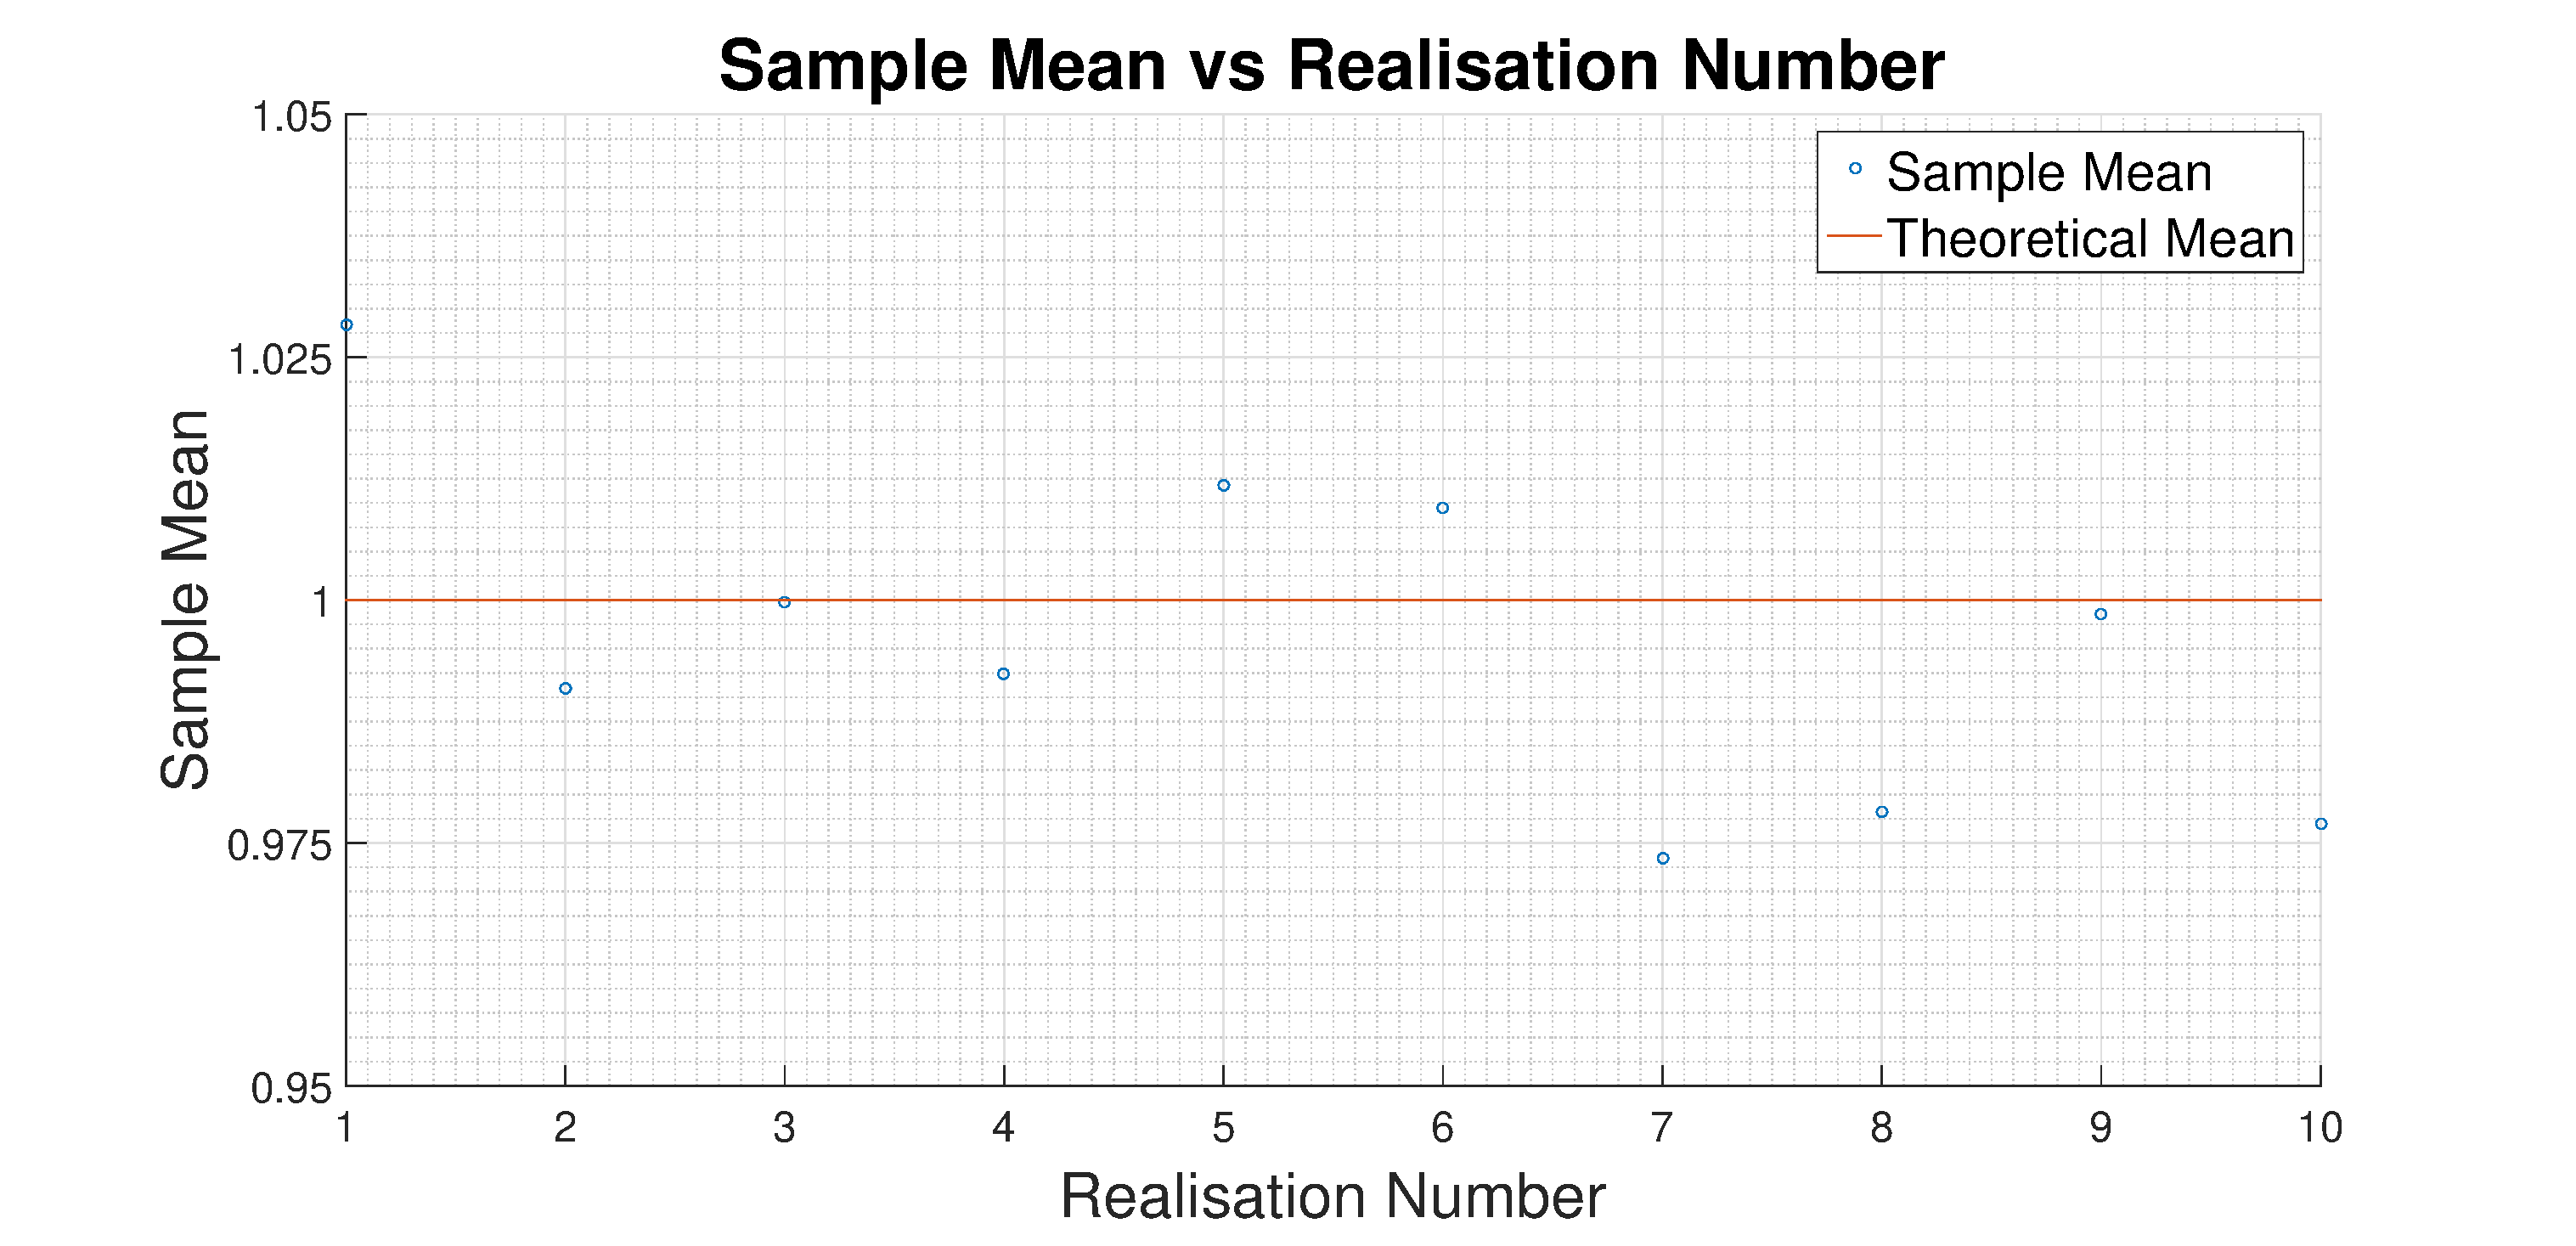
\includegraphics[width=0.49\textwidth]{sample_mean_vs_realisation_number_randn}
\includegraphics[width=0.49\textwidth]{sample_standard_deviation_vs_realisation_number_randn}
\caption{Sample mean and sample standard deviation for each member of the ensemble, samples considered have a Gaussian distribution}
\end{figure}

Similar to the results obtained when the samples were drawn from a uniform distribution, the means and standard deviations hover around their theoretical values. This further corroborates the fact that the sample mean and the sample standard deviation are unbiased estimators.\\

Next, the PDF of the underlying distribution that our samples are drawn from, which in this case is the Guassian distribution, is estimated. Again as a performance measure, a plot of the PDF of a zero-mean unit standard deviation Gaussian distribution is included.

\begin{figure}[H]
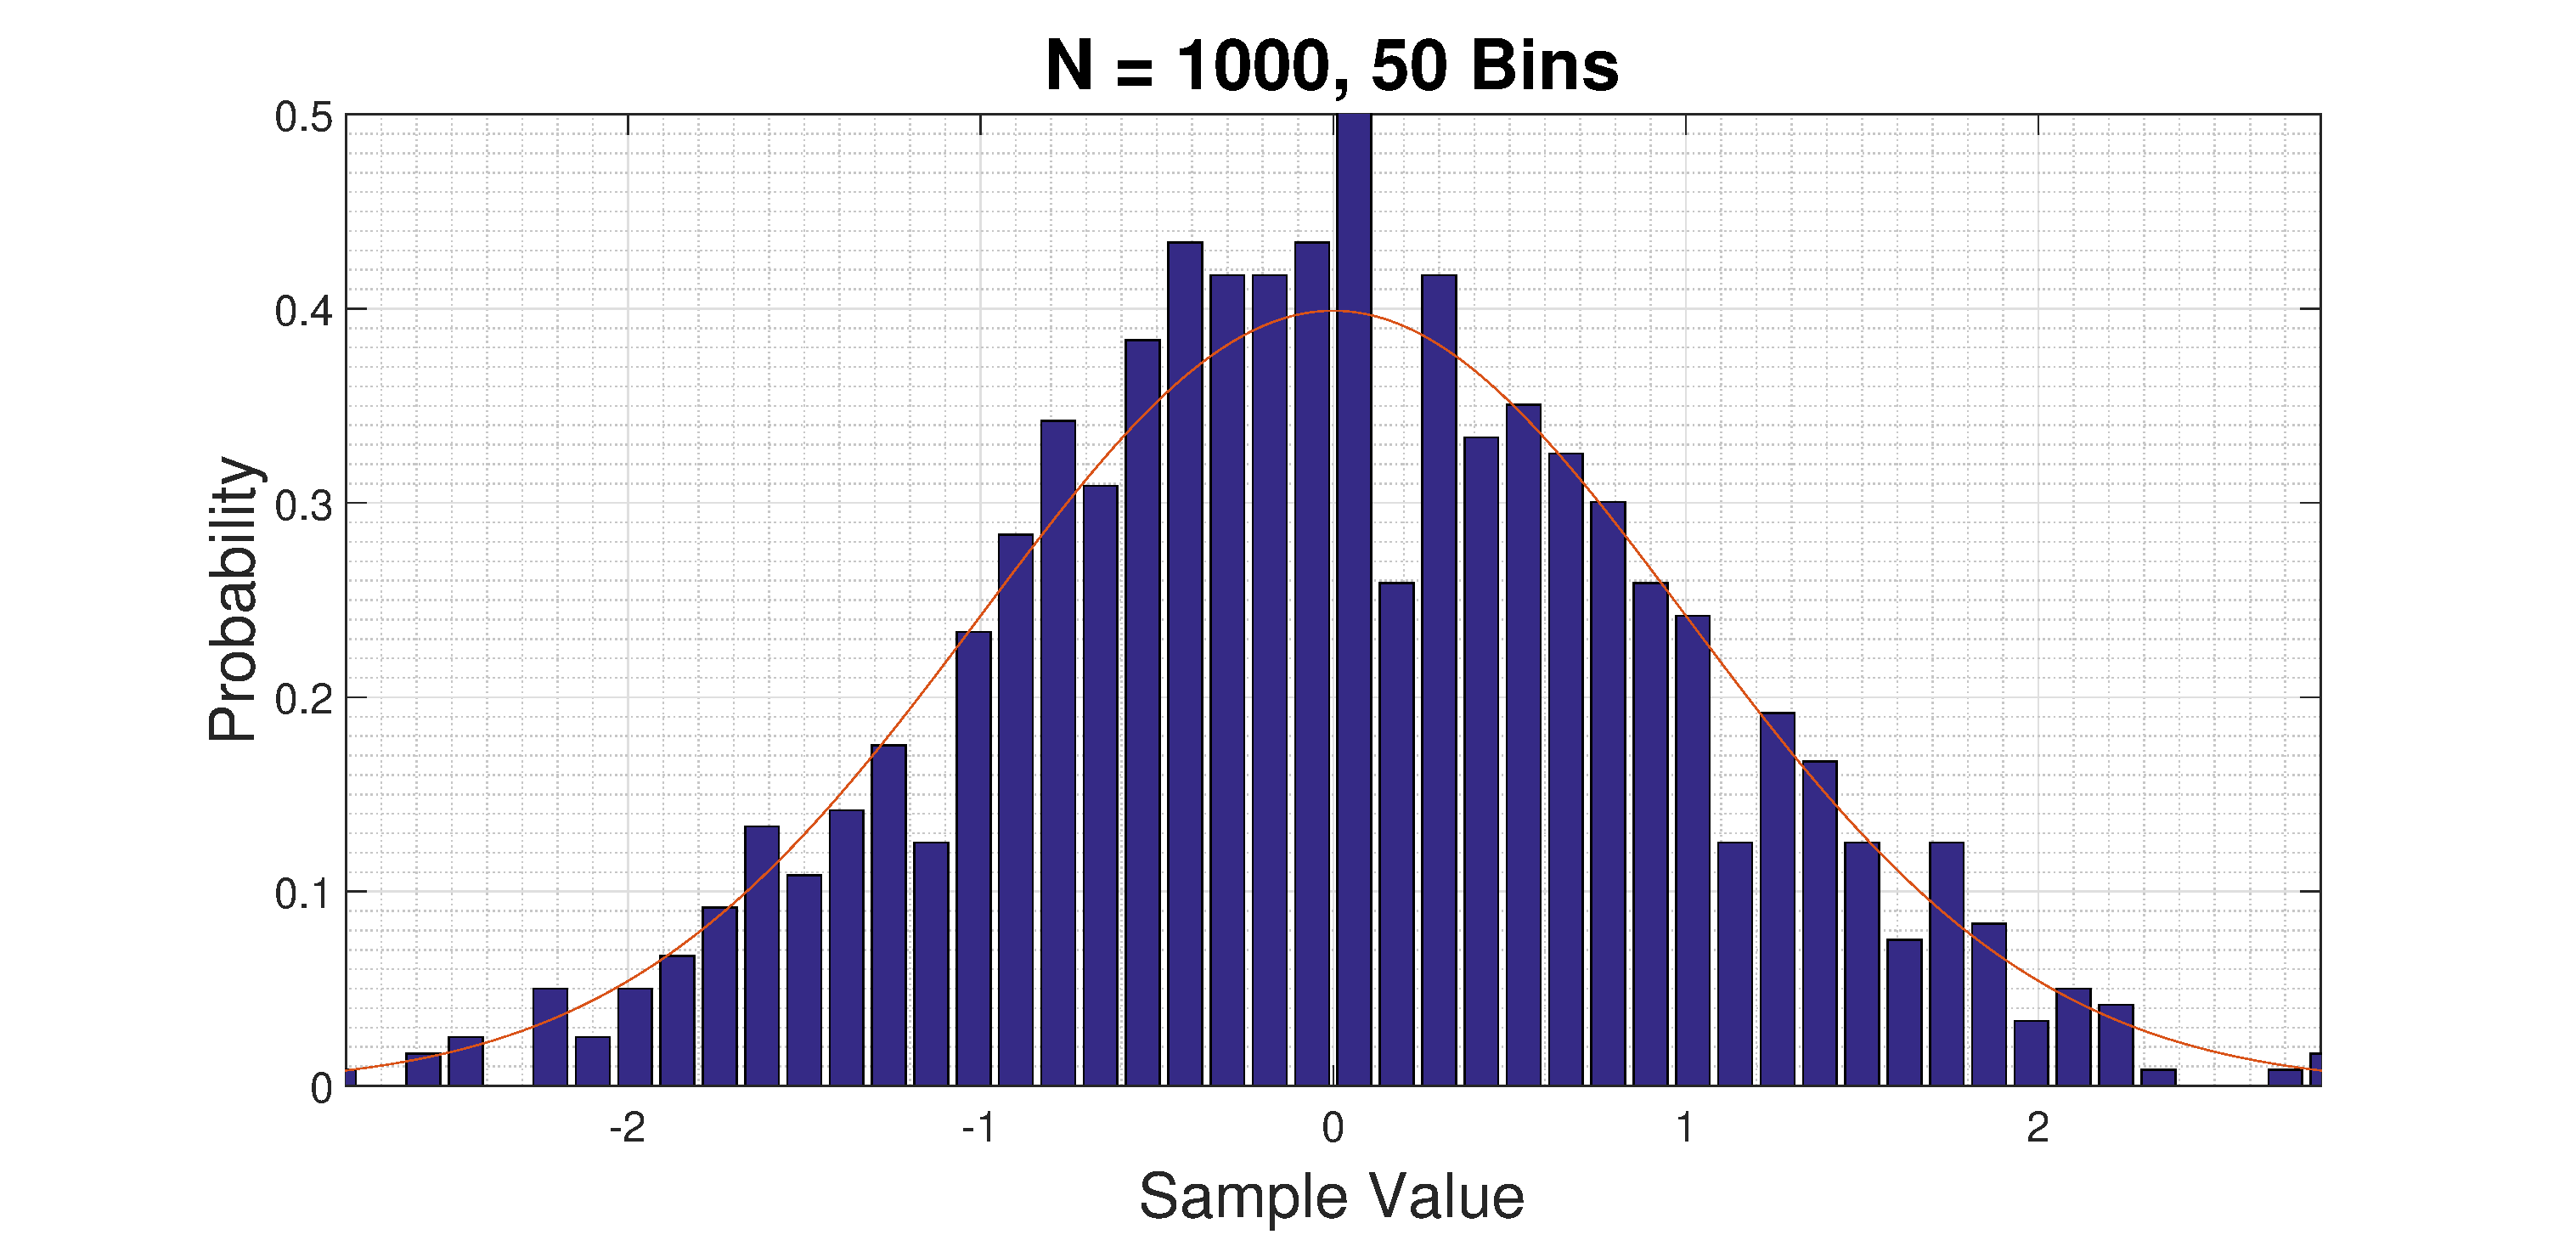
\includegraphics[width=0.49\textwidth]{N_1000_B_50_randn}
\includegraphics[width=0.49\textwidth]{N_1000_B_100_randn}
\caption{PDF underlying random samples using {\tt hist}, varying bin size}
\end{figure}

The number is bins is clearly related to the resolution of the estimate whereas the number of samples will determine the estimator's accuracy.

\begin{figure}[H]
\includegraphics[width=0.49\textwidth]{N_100000_B_100_randn}
\includegraphics[width=0.49\textwidth]{N_1000000_B_100_randn}
\caption{PDF underlying random samples using {\tt hist}, varying sample size}
\end{figure}


\newpage
\subsection{Stochastic Processes}
A random process that has time-invariant statistical properties is referred to as statistically stationary. White Gaussian noise, $w[n]$ is an example of a stationary process whereas a sine wave of the form $w[n]sin(2\pi Fn)$ is not stationary as the expected value of the process depends on the time instance at which the process is being observed. 

A random process processes ergodicity if a single realisation of the process of sufficient length is enough to determine the statistical properties of the process. For an ergodic signal, the time average will approach the ensemble average as the number of samples are increased. To fully grasp the idea of ergodicity, we consider a process, that once initialised at a random value $x_{i}$, which is a single realisation of the random variable $X\sim \mathcal{U}(0,1)$, will retain its value for all time. The time average of this signal will be $x_{i}$, regardless of the number of samples that are considered. The time average however does not reveal the randomness inherent in the process. This process is thus, not ergodic. To formalise the concept of ergodicity, a mathematical description of a ergodic process is provided in equation (\ref{eq:ergodic_process}).\\ 

\begin{equation}\label{eq:ergodic_process}
    \lim_{N\to\infty}\hat{m}_{x}(N) = m_{x}\\
\end{equation}

In equation (\ref{eq:ergodic_process}), $\hat{m}_{x}$ is the sample mean of the signal, which can be thought of as the time-average of the random process, and $m_{x}$ is the ensemble average which is calculated by averaging across realisations of the random process. The ensemble average is mathematically formalised in equation (\ref{eq:ensemble_average}), where $x_{i}[n]$ is the n\textsuperscript{th} sample of the i\textsuperscript{th} ensemble.

\begin{equation}\label{eq:ensemble_average}
    m_{x} = \frac{1}{M}\sum_{i=1}^{M} x_{i}[n]    
\end{equation}


1. The ensemble mean and standard deviations are graphed for each of the three process as a function of the sample number.

\begin{figure}[H]
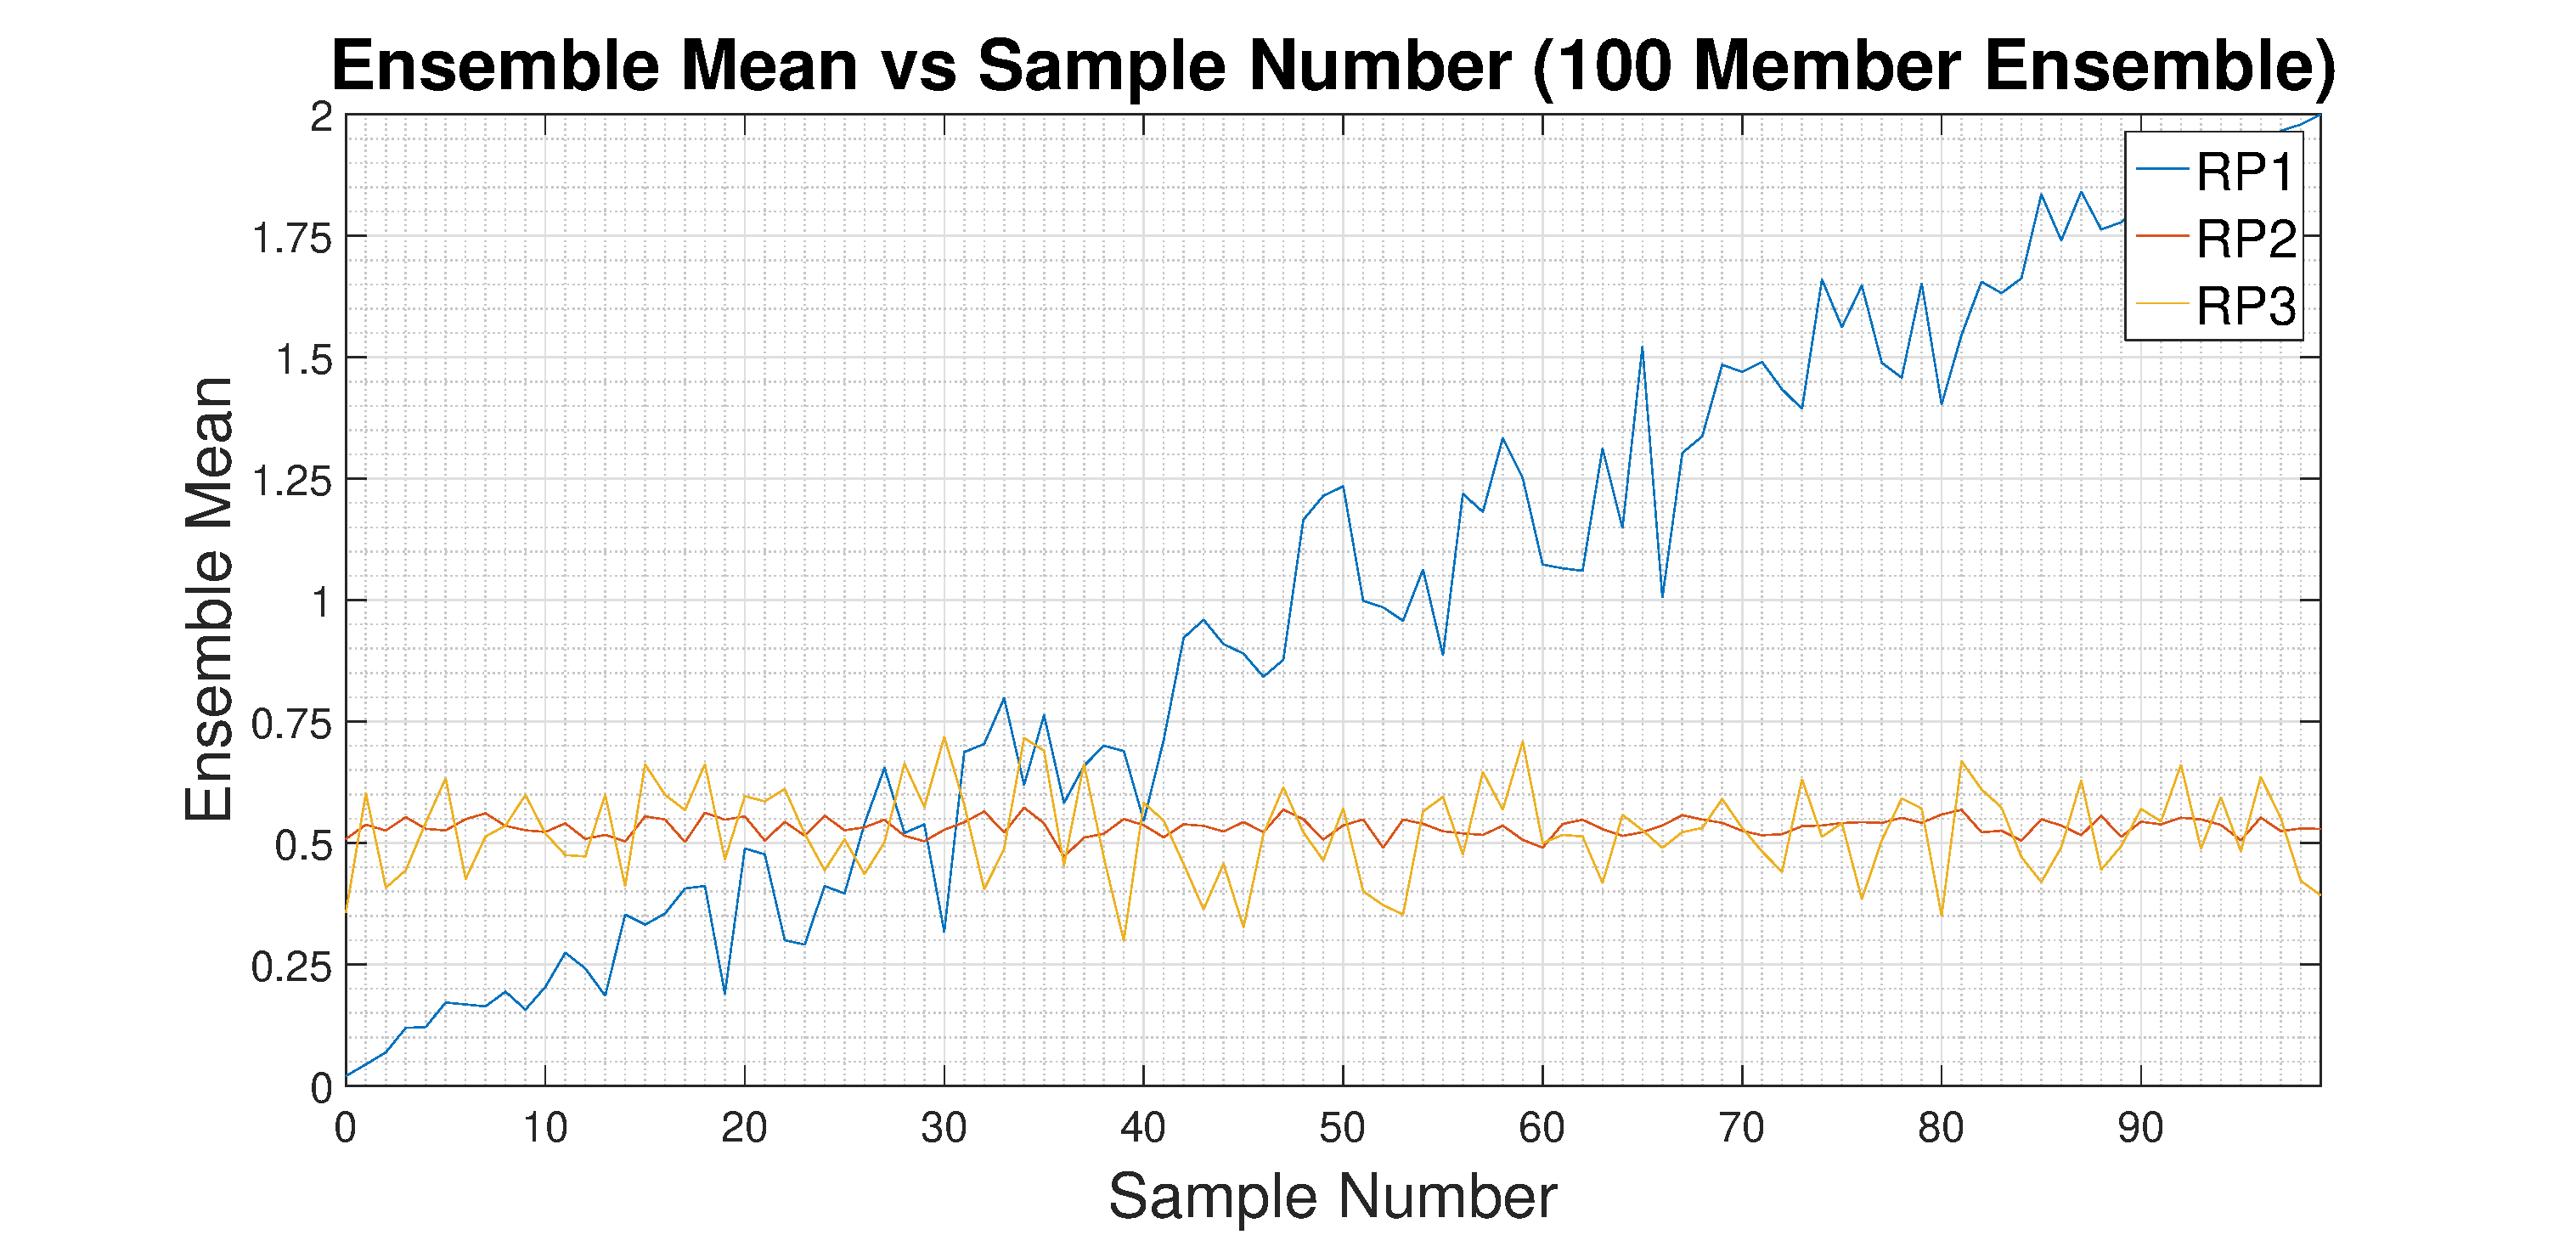
\includegraphics[width=0.49\textwidth]{ensemble_means}
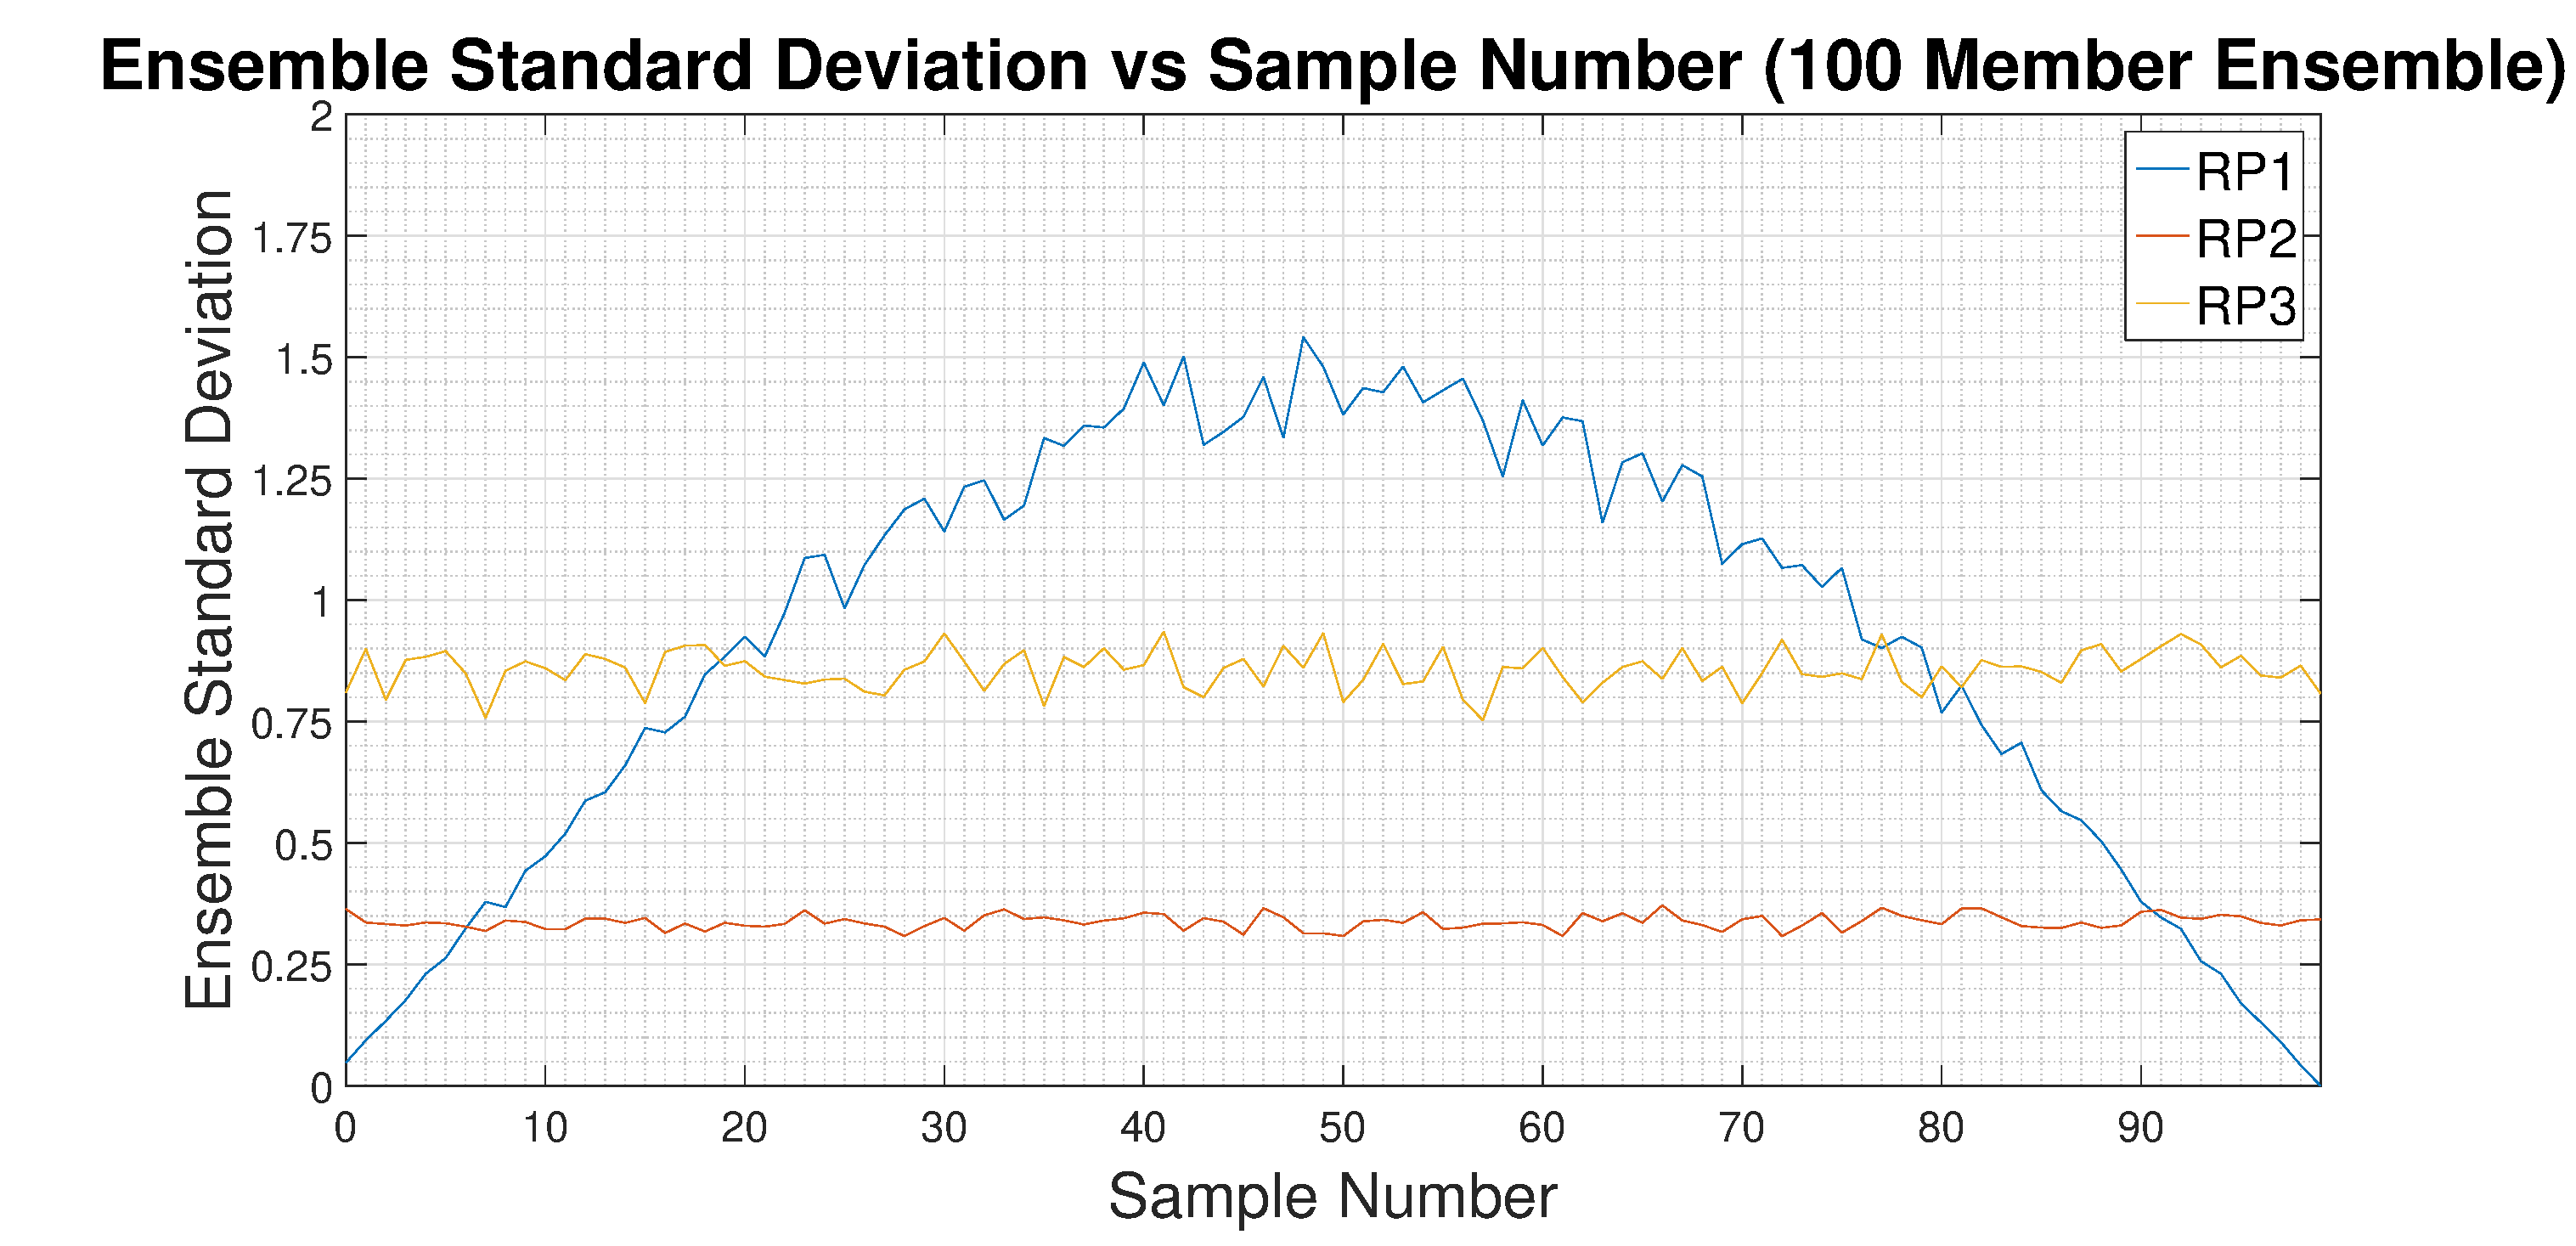
\includegraphics[width=0.49\textwidth]{ensemble_standard_deviations}
\caption{Ensemble means and standard deviations of each of the three random processes}
\end{figure}

It is clear that for random process 1, the mean and standard deviation are not time-invariant. There is an increasing trend in process's mean and a parabolic trend in its standard deviation. Thus, it is not a stationary process. Random process 2 and 3 are stationary as their ensemble means and standard deviations do not follow any trend and hover around a single value, making them time-invariant.\\

2. A 4-member ensemble is generated for each of the random processes and the sample mean and sample standard deviation is graphed for each member of the ensemble.

\begin{figure}[H]
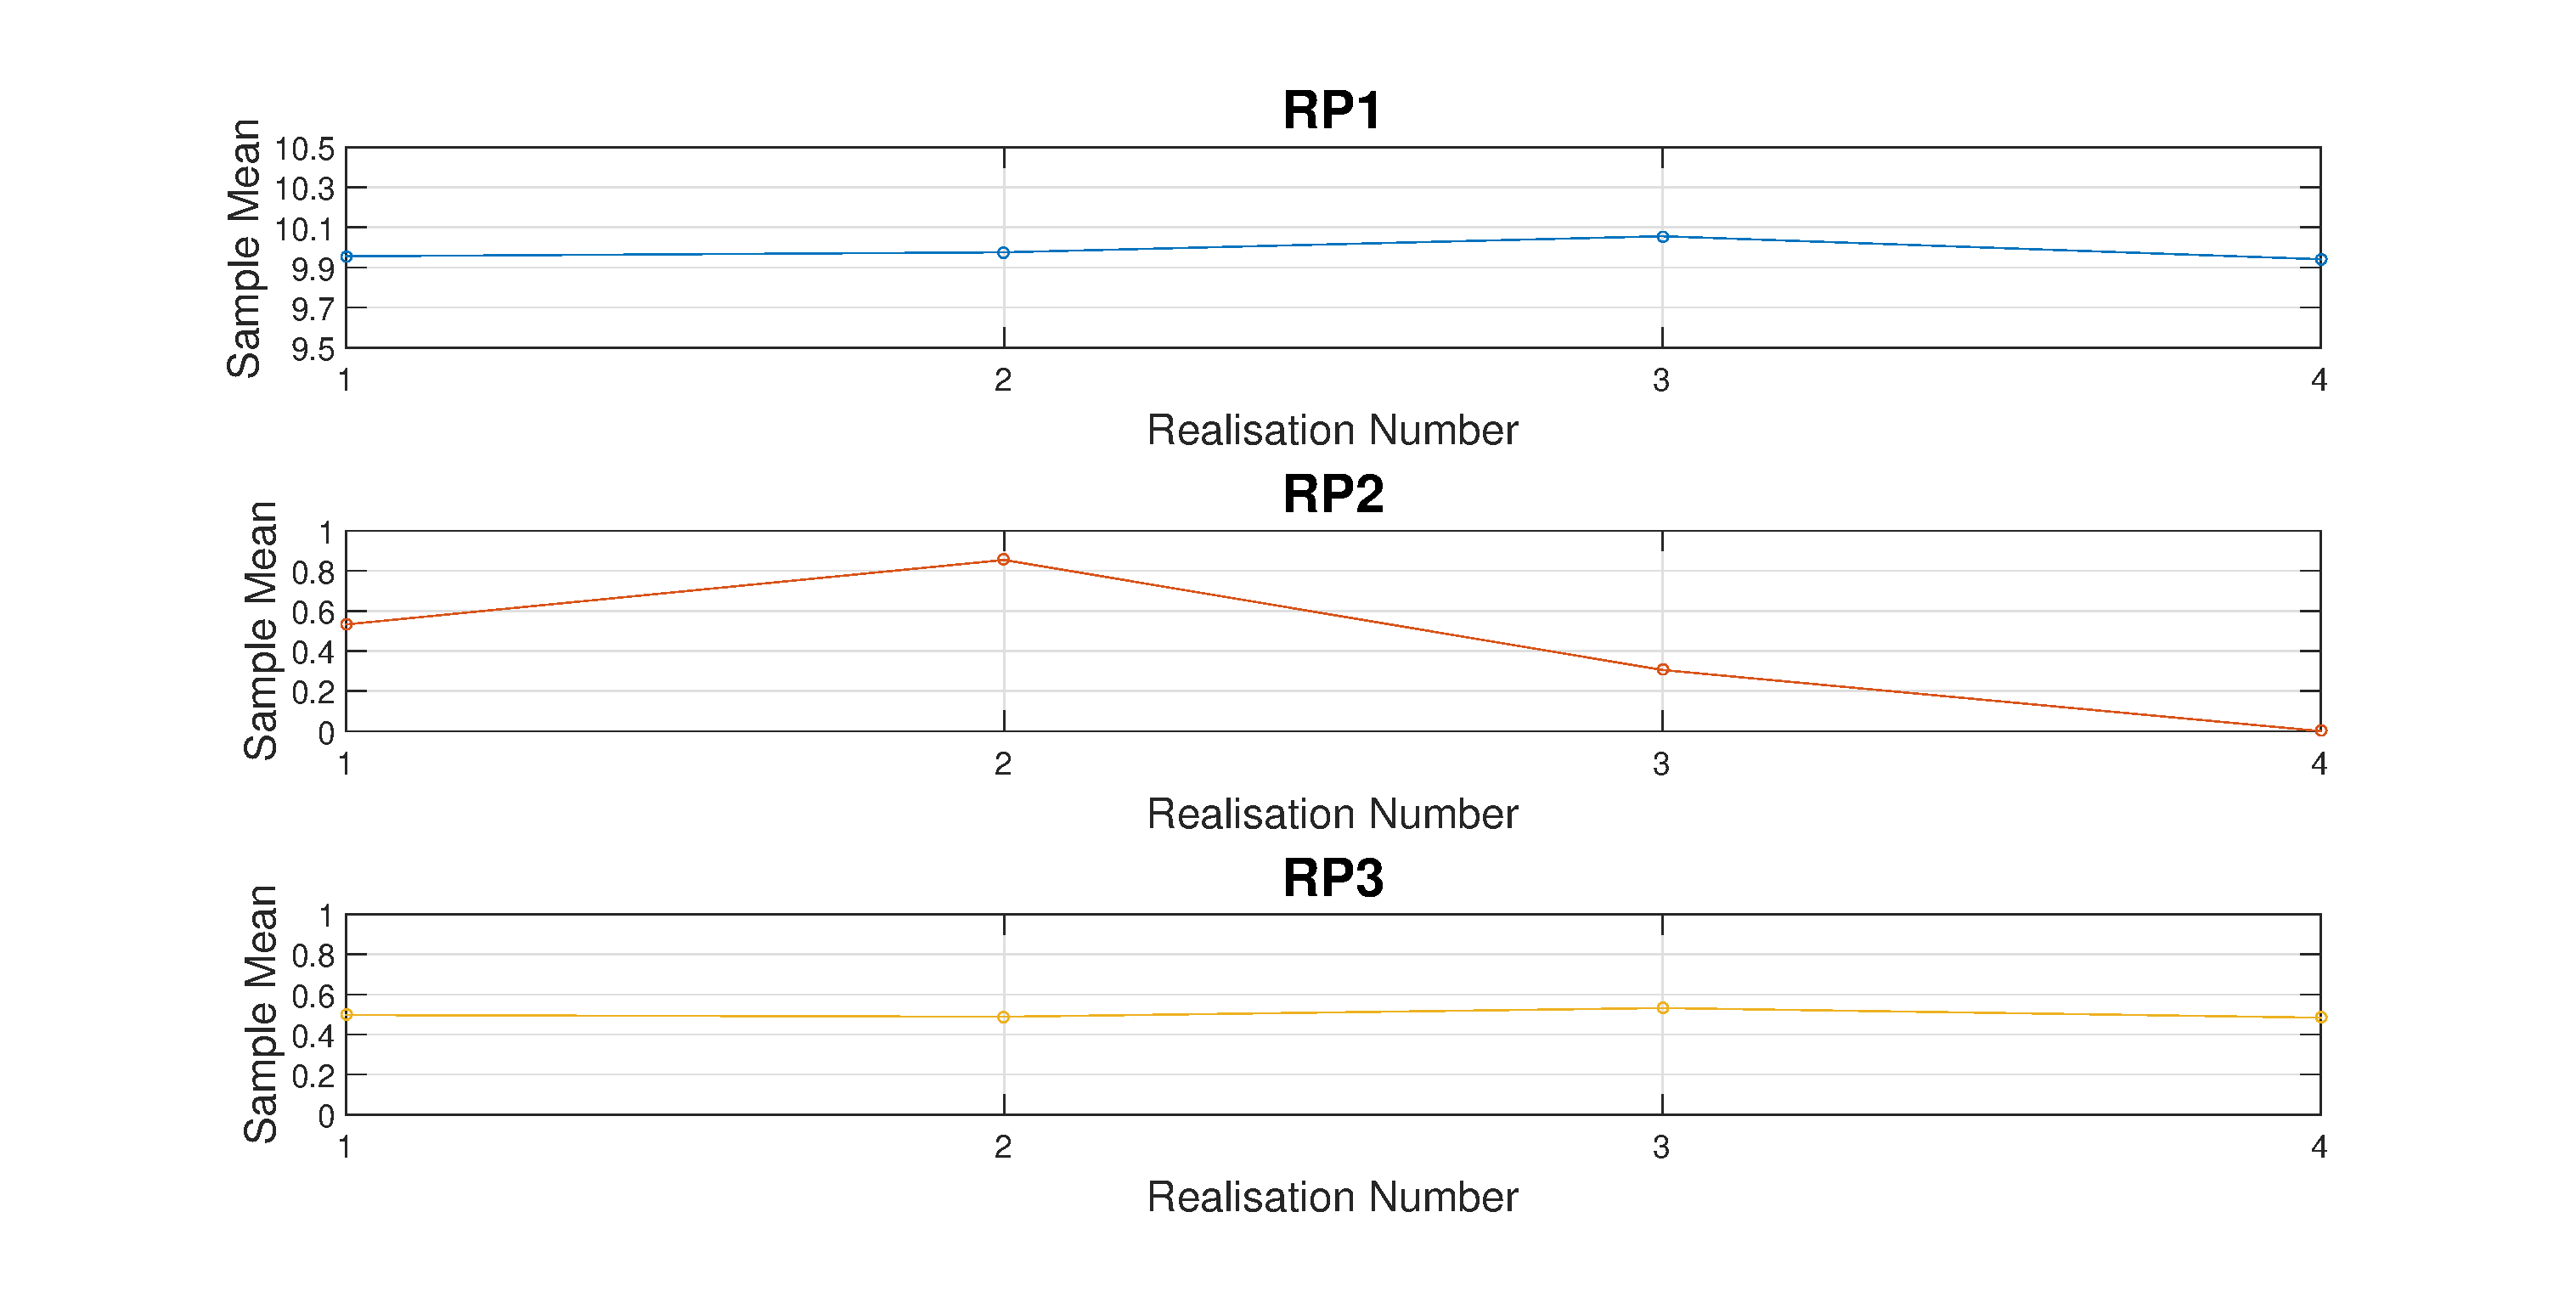
\includegraphics[width=0.49\textwidth]{sample_mean_of_each_realisation}
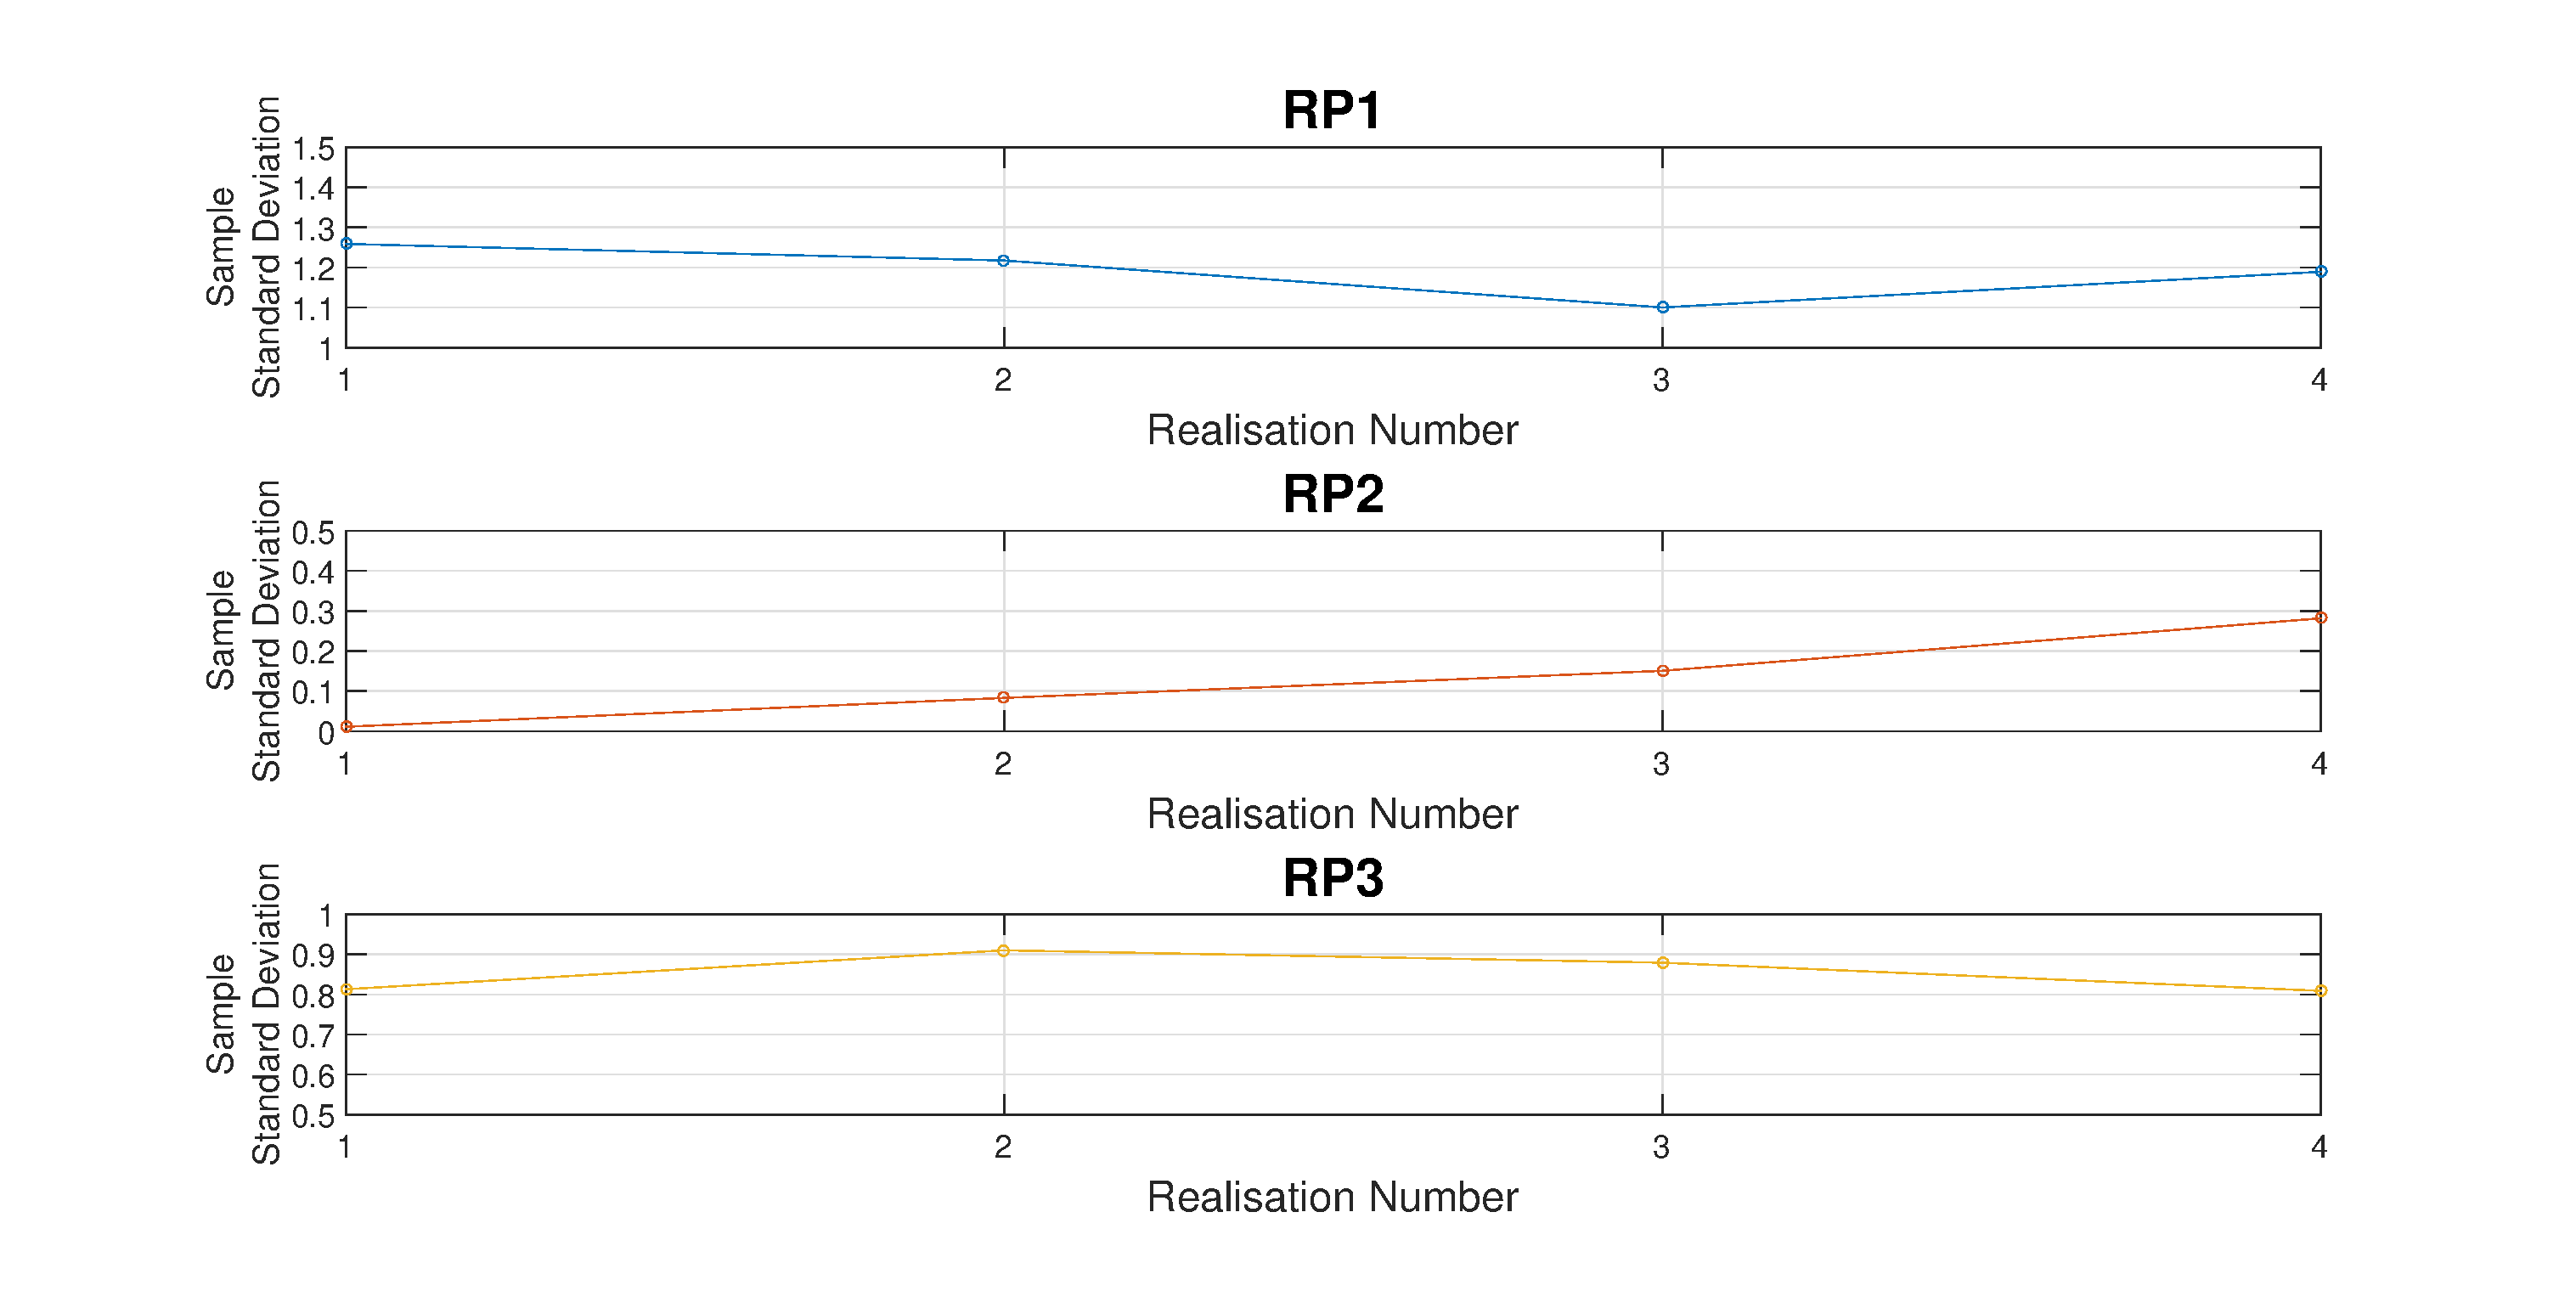
\includegraphics[width=0.49\textwidth]{sample_standard_deviation_of_each_realisation}
\caption{Sample means and standard deviations of each realisation in the 4-member ensemble}
\label{fig:sample_mean_and_standard_deviation_of_each_realisation}
\end{figure}

As discussed above, for an ergodic process, the sample mean should approach the ensemble mean. This implies that multiple realisations, of infinite length, of an ergodic process should have the same sample mean. The plots above show that the sample means for different realisations of random process 2 vary by significantly more than that of other processes\footnote{in Figure \ref{fig:sample_mean_and_standard_deviation_of_each_realisation} all graphs have the same scale}. It is hard to conclude, at this point, if this large variation is due to the fact that we are dealing with finite length sequences or that random process 2 does not possess ergodicity. We can however conclude that since random process 1 is not stationary, the ensemble average is time variant and thus it cannot possess ergodicity. In addition, since the time-averages of multiple realisations of random process 3 are approximately the same, it is highly likely that random process 3 is ergodic. Ergodicity will be conclusive proven once mathematical descriptions of the processes are considered.\\

3. Mathematical descriptions of the 3 random processes are provided below.\\

i. \textit{\underline{Random Process 1}}\\

Random Process 1 is defined by equation \ref{eq:rp1}, where $Z$ is a random variable such that $Z \sim \mathcal{U}(0,1)$,

\begin{equation}
    x[n] = 5(Z-0.5)sin(\frac{\pi n}{N}) + 0.02n\label{eq:rp1} 
\end{equation}

To find the theoretical mean of the random process,

\begin{align}
     \mathbb{E}\{x[n]\} &= \mathbb{E}\{5(Z-0.5)sin(\frac{\pi n}{N}) + 0.02n\}\nonumber\\
                        &= 5\mathbb{E}\{Z-0.5)\}sin(\frac{\pi n}{N}) + \mathbb{E}\{0.02n\}\nonumber\\
                        &= 5(0.5-0.5)sin(\frac{\pi n}{N}) + 0.02n\nonumber\\
                        &= 0.02n \label{eq:random_process_1_mean}
\end{align}

To find the theoretical variance of the random process,

\begin{align}
    Var(x[n])   &= \mathbb{E}\{x[n]^{2}\} - \mathbb{E}\{x[n]\}^{2}\nonumber\\
                &= \mathbb{E}\{(5(Z-0.5)sin(\frac{\pi n}{N}) + 0.02n)^{2}\} - (0.02n)^{2}\nonumber\\
                &= \mathbb{E}\{25(Z-0.5)^{2}sin^{2}(\frac{\pi n}{N})\} + \mathbb{E}\{0.2n(Z-0.5)sin(\frac{\pi n}{N})\} + \mathbb{E}\{(0.02n)^{2}) - (0.02n)^{2}\nonumber\\
                &= 25\mathbb{E}\{(Z-0.5)^2\}sin^{2}(\frac{\pi n}{N}) + 0.2n(0.5-0.5)sin(\frac{\pi n}{N}) + (0.02n)^{2} - (0.02n)^n\nonumber\\
                &= 25sin^{2}(\frac{\pi n}{N})(\mathbb{E}\{Z^{2}\}-\mathbb{E}\{Z\}+(0.5)^2)\nonumber\\
                &= 25sin^{2}(\frac{\pi n}{N})(\nicefrac{1}{3}-0.5+0.25)\nonumber\\
                &= \frac{25}{12}sin^{2}(\frac{\pi n}{N})\nonumber
\end{align}
It is important to note that the square of a uniformly distributed random variable $Z\sim \mathcal{U}(0,1)$ is a another random variable $Y$ that has the PDF which is defined as $\frac{1}{2\sqrt{Z}}$. The expectation of $Y$ is equal to $\frac{1}{3}$. As such the standard deviation of random process 1 is,

\begin{equation}
    \sigma_{RP1} = \frac{5}{\sqrt{12}}sin(\frac{\pi n}{N})\label{eq:random_process_1_standard_deviation}
\end{equation}

From equations (\ref{eq:random_process_1_mean}) and (\ref{eq:random_process_1_standard_deviation}), it is clear that random process 1 is not stationary. Both its mean and its standard deviation are time variant. The mathematical description corroborates the earlier conjecture that random process 1 is not stationary.\\ 

ii. \textit{\underline{Random Process 2}}\\

Random Process 2 is defined by the equation (\ref{eq:random_process_2}), where $M$, $A$ and $Z$ are random variables that are uniformly distributed. $M$ and $A$ are time-invariant but change with each realisation of the random process whereas $Z$ varies both with time and with realisation.

\begin{equation}\label{eq:random_process_2}
    x[n] = M(\mathcal{U}(0,1)-0.5) + A
\end{equation}

To find the theoretical mean of the random process,

\begin{align}
    \mathbb{E}\{x[n]\}  &= \mathbb{E}\{M(Z-0.5) + A\}\nonumber\\
                        &= \mathbb{E}\{M\}\mathbb{E}\{Z-0.5\} + \mathbb{E}\{A\}\nonumber\\
                        &= (0.5)(0.5-0.5) + (0.5)\nonumber\\
                        &= 0.5 \label{eq:random_process_2_mean}
\end{align}

To find the theoretical variance of the random process,

\begin{align}
    Var(x[n])   &= \mathbb{E}\{(M(Z-0.5) + A)^{2}\} - \mathbb{E}\{ M(Z-0.5) + A\}^{2}\nonumber\\
                &= \mathbb{E}\{M^{2}(Z-0.5)^{2} + 2MA((Z-0.5) + A^{2}\} - (0.5)^{2}\nonumber\\
                &= \mathbb{E}\{M^{2}\}\mathbb{E}\{(Z-0.5)^{2}\}+2\mathbb{E}\{M\}\mathbb{E}\{A\}\mathbb{E}\{Z-0.5)\}+\mathbb{E}\{A^{2}\} - 0.25\nonumber\\
                &= (\frac{1}{3})(\frac{1}{12})+2(0.5)(0.5)(0.5-0.5)+(\frac{1}{3}) - 0.25\nonumber\\
                &= \frac{1}{9}\nonumber
\end{align}

As such, the standard deviation of random process 2 is,

\begin{equation}
    \sigma_{RP2} = \frac{1}{3} \label{eq:random_process_2_standard_deviation}
\end{equation}

From equations (\ref{eq:random_process_2_mean}) and (\ref{eq:random_process_2_standard_deviation}), it is clear that random process 2 is stationary. However, equation (\ref{eq:random_process_2}) shows that the process is not ergodic. The sample mean of one realisation of the random process approach $A_{i}$, which is just one realisation of the random variable $A$. No matter how many samples we take of one realisation of random process 2, we will not be able to determine the random behavior inherent in $A$ and thus calculate the mean of the random process.\\

iii. \textit{\underline{Random Process 3}}\\

Random Process 3 is defined by the following equation, where $Z$ is a random variable such that $Z \sim \mathcal{U}(0,1)$,

\begin{equation}\label{eq:random_process_3}
    x[n] = 3(Z-0.5) + 0.5
\end{equation}


To find the theoretical mean of the random process,

\begin{align}
    \mathbb{E}\{x[n]\}  &= \mathbb{E}\{3(Z-0.5) + 0.5\}\nonumber\\
                        &= 3\mathbb{E}\{(Z-0.5)\} +\mathbb{E}\{0.5\}\nonumber\\
                        &= 3(0.5-0.5) + 0.5\nonumber\\
                        &= 0.5 \label{eq:random_process_3_mean}
\end{align}

To find the theoretical variance of the random process,

\begin{align}
    Var(x[n])   &= \mathbb{E}\{(3(Z-0.5) + 0.5)^{2}\} - \mathbb{E}\{3(Z-0.5) + 0.5\}^{2}\nonumber\\
                &= 9\mathbb{E}\{(Z-0.5)^2\} +3\mathbb{E}\{(Z-0.5)\} +\mathbb{E}\{(0.5)^{2}\}- (0.5)^{2}\nonumber\\
                &= \frac{9}{12} + 3(0.5-0.5) + (0.5)^{2} - (0.5)^{2}\nonumber\\
                &= \frac{9}{12}\nonumber
\end{align}

As such, the standard deviation of random process 3 is,

\begin{equation}
    \sigma_{RP3} = \frac{\sqrt{3}}{2} \label{eq:random_process_3_standard_deviation}
\end{equation}

From equations (\ref{eq:random_process_3_mean}) and (\ref{eq:random_process_3_standard_deviation}), it is clear that random process 3 is stationary. Equation (\ref{eq:random_process_3}) shows that random process 3 is ergodic and the mean and standard deviation can be calculated from one sufficiently long realisation of the random process.

\subsection{Estimation of probability distributions}\label{sec:pdf_m}

\begin{figure}[H]
\centering{}
\includegraphics[width=0.49\textwidth]{probability_density_function}
\caption{Estimated PDF of Gaussian random variable}
\label{fig:estimation_of_gaussian}
\end{figure}

1. Figure \ref{fig:estimation_of_gaussian} shows that the file {\tt pdf.m} works as expected. As a performance measure, a plot of the PDF of a zero-mean, unit standard deviation, Gaussian distribution is included.\\

2. The only random process that is both stationary and ergodic is random process 3. Random process 3 can be represented by a single random variable $X$ that has a uniform distribution. More specifically $X\sim \mathcal{U}(-1,2)$. Figure \ref{fig:pdf_of_RP3} shows the estimated PDF approximated using {\tt pdf.m}. Increasing the sample size significantly improves the estimate. As a performance measure, the theoretical PDF has been included.

\begin{figure}[H]
\centering{}
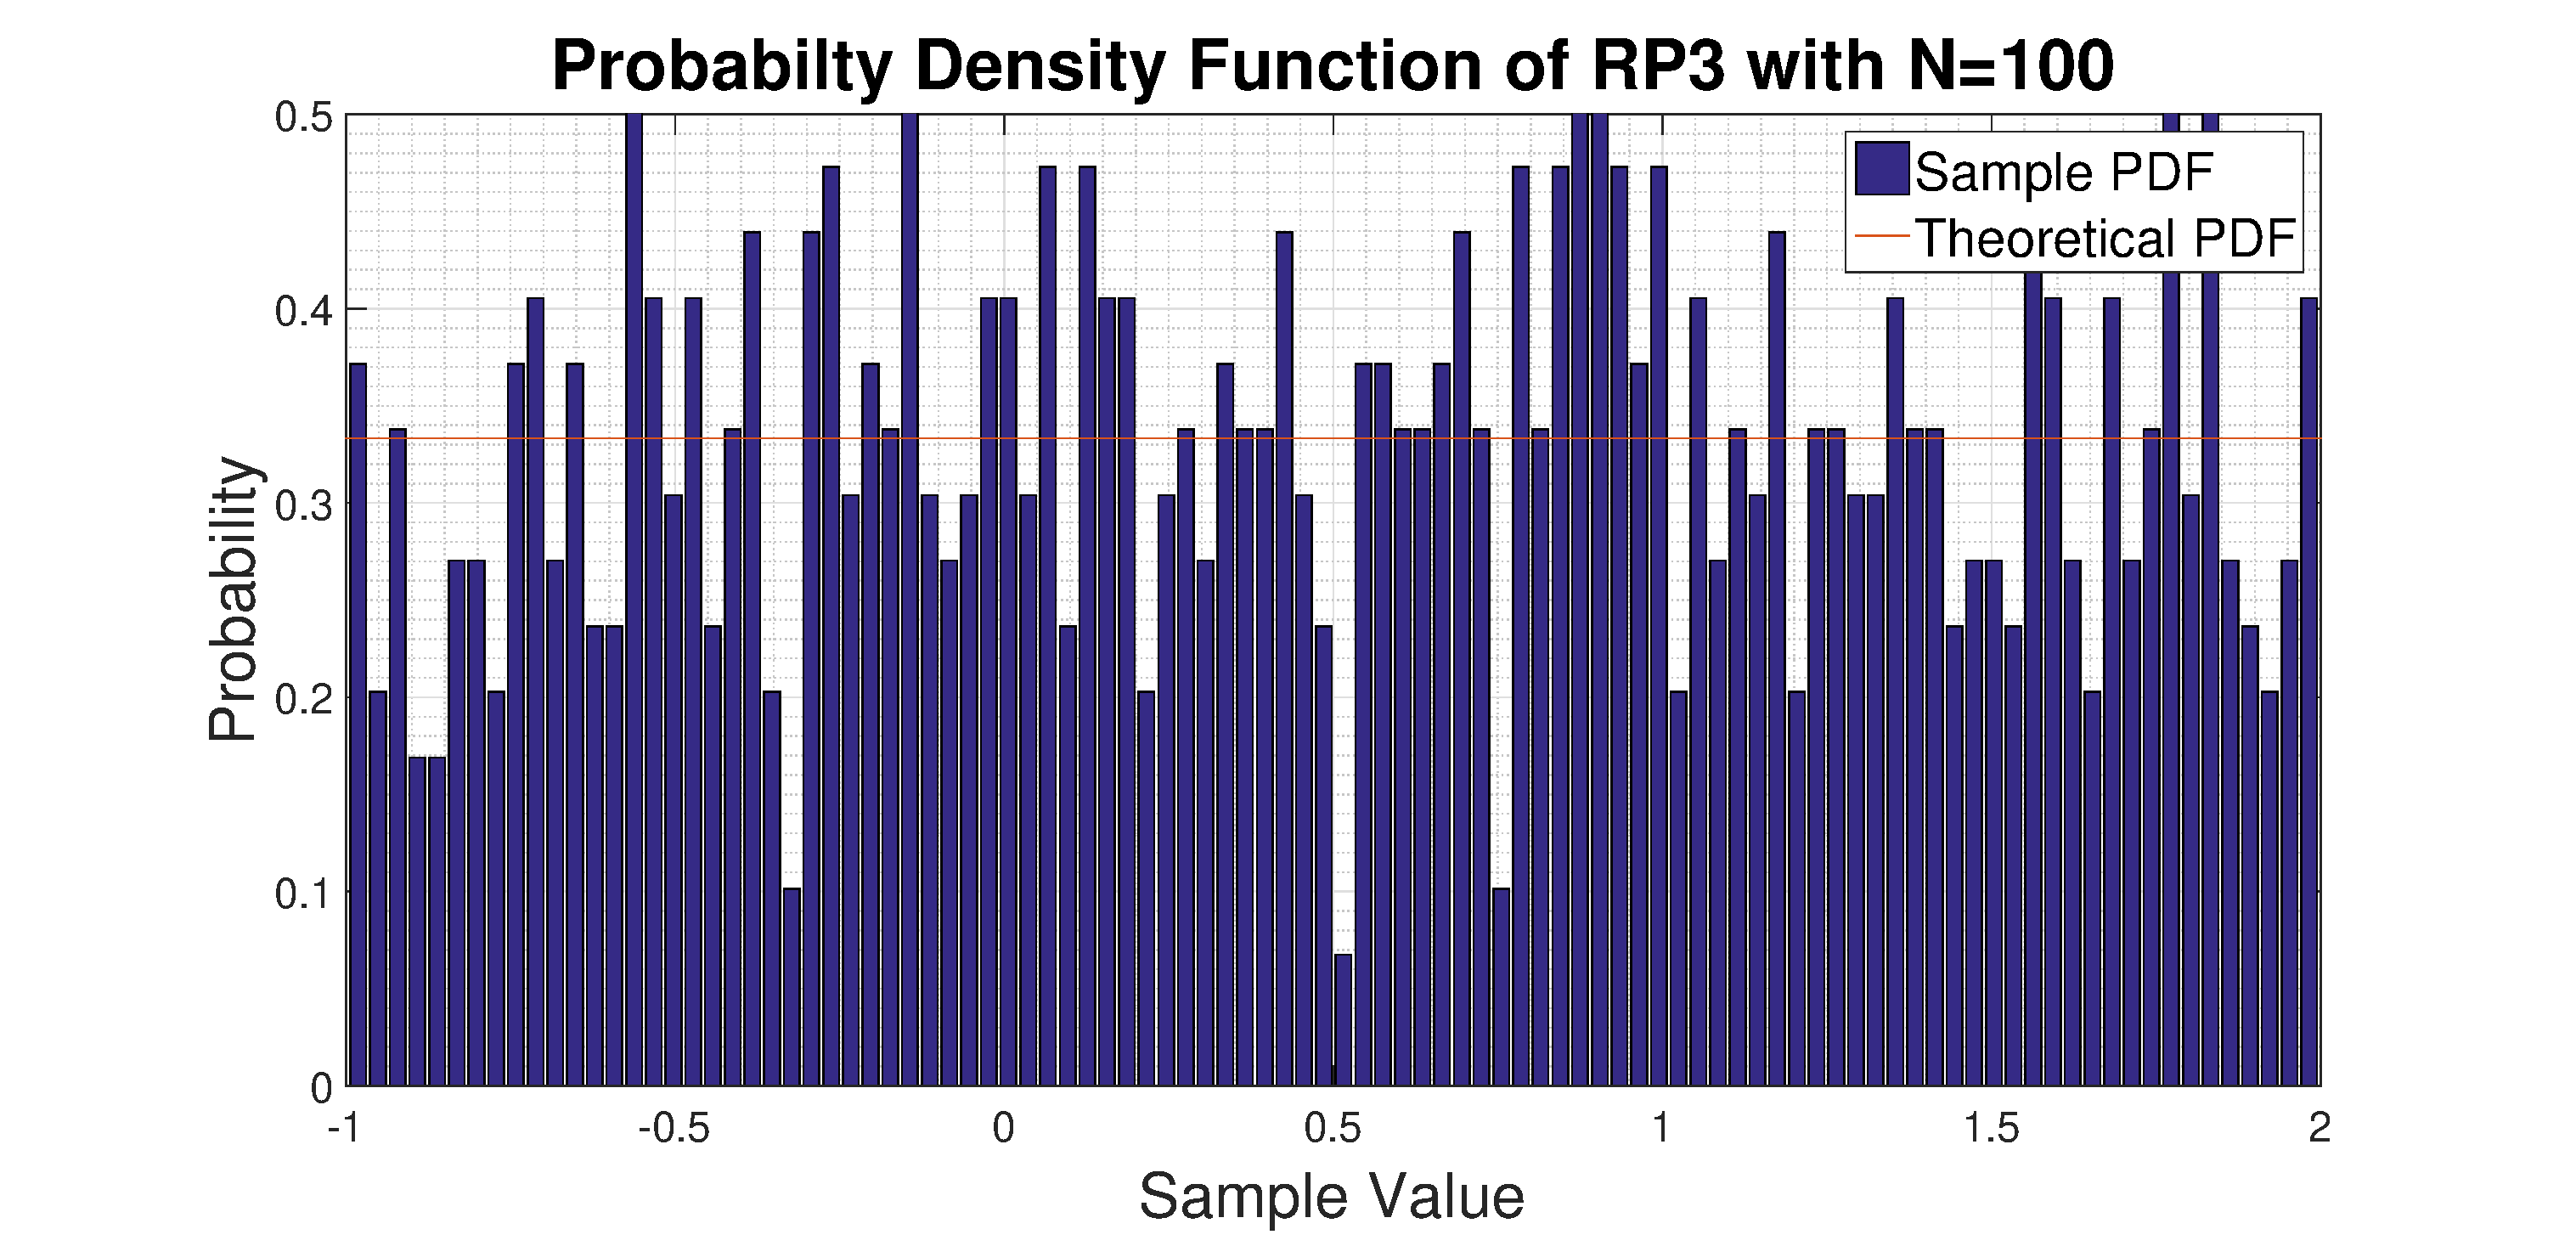
\includegraphics[width=0.49\textwidth]{pdf_of_RP3_1}
\includegraphics[width=0.49\textwidth]{pdf_of_RP3_2}
\caption{Estimated PDF of random process 3}
\label{fig:pdf_of_RP3}
\end{figure}
\newpage
\section{Linear Stochastic Modelling}
\subsection{ACF of Uncorrelated Sequences}\label{sec:acf_uncorrelated}

1. The unbiased estimate of the ACF is graphed in figure \ref{fig:acf_uncorrelated}. All real signals have symmetric ACF, i.e, the ACF is an even function if the input signal is real. If the signal is complex valued, the ACF will be a Hermitian function; a Hermitian Function is defined as one in which $R(\tau) = R^{*}(-\tau)$. The ideal ACF of white noise should consist of a dirac delta function at $\tau = 0$ and should be $0$ elsewhere. This would indicate that the samples are completely uncorrelated and thus, random. The peak at $\tau = 0$ is present in the unbiased estimate, however the estimate is not $0$ elsewhere. 

\begin{figure}[H]
    \centering
    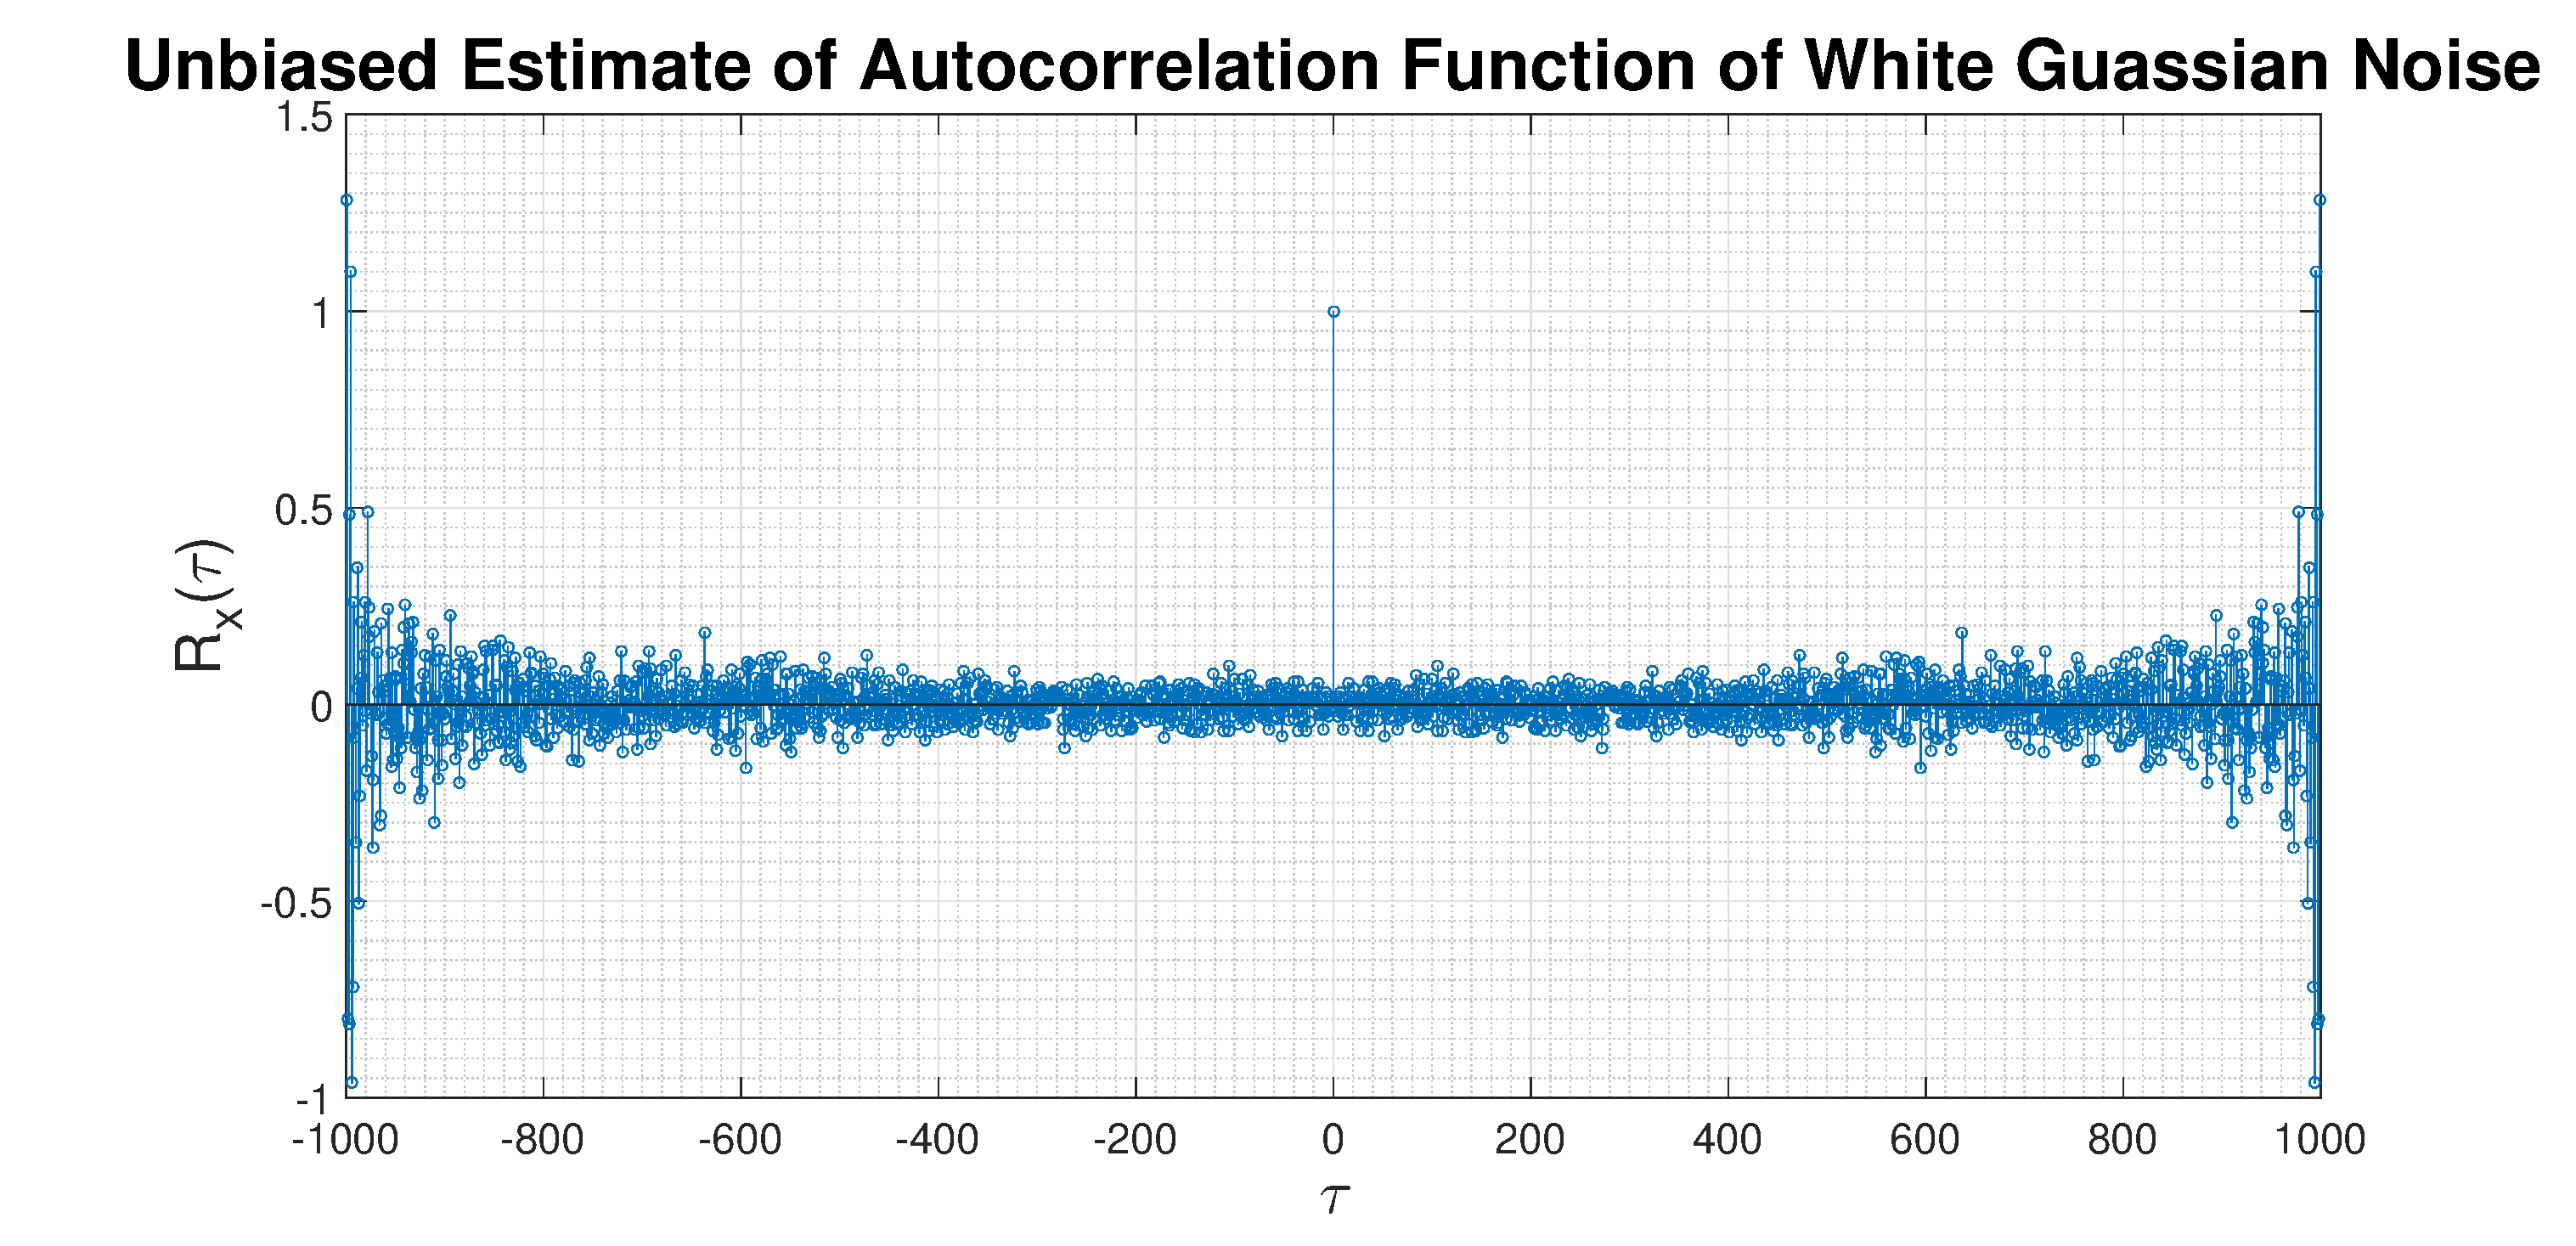
\includegraphics[width=0.49\textwidth]{acf_uncorrelated}
    \includegraphics[width=0.49\textwidth]{acf_uncorrelated_zoom}
    \caption{Unbiased estimate of ACF of uncorrelated sequences}
    \label{fig:acf_uncorrelated}
\end{figure}

2. Observing the zoomed plot, it is clear that the estimate of the ACF is very close to the ideal ACF described above. There is a large peak at $\tau = 0$ and for other values of $\tau$, the estimate is approximately 0. This is however not the case for large values of $\tau$ where the estimate is extremely large, often larger in magnitude than the peak at $\tau = 0$.


\begin{align}
    \hat{R_{X, \ unbiased}(\tau)} &= \frac{1}{(N-|\tau|)}\sum_{n=0}^{N-|\tau|-1}x[n]x[n+\tau]\label{eq:unbiased_estimate_ACF}\\
    Var(\hat{R_{X, \ unbiased}(\tau)}) &= \frac{1}{(N-|\tau|)^2}Var\bigg(\sum_{n=0}^{N-|\tau|-1}x[n]x[n+\tau]\bigg)\label{eq:unbiased_estimate_ACF_var}
\end{align}

3. The unbiased estimate of the ACF has the form defined in equation (\ref{eq:unbiased_estimate_ACF}) and the estimator's variance is defined in equation (\ref{eq:unbiased_estimate_ACF_var}). Notice that the estimator has a scaling factor of $\frac{1}{N-|\tau|}$ to ensures that the estimator is unbiased; the mean of the estimator is independent of $\tau$. Although the estimator is unbiased, the variance of the estimator increases with $\tau$. As such, the shape of the ACF for large $\tau$ is unreliable.

\begin{align}
    \hat{R_{X, \ biased}(\tau)} &= \frac{1}{N}\sum_{n=0}^{N-|\tau|-1}x[n]x[n+\tau]\label{eq:biased_estimate_ACF}\\
     Var(\hat{R_{X, \ biased}(\tau)}) &= \frac{1}{N^2}Var\bigg(\sum_{n=0}^{N-|\tau|-1}x[n]x[n+\tau]\bigg)\label{eq:biased_estimate_ACF_var}
\end{align}

The form of the biased estimator is presented in equation (\ref{eq:biased_estimate_ACF}). Observing the form of the biased estimator, it is clear that the values calculated at large $\tau$ are given lower weightings. The ACF for large $\tau$ is calculated with a smaller number of samples; the limits of the summation decreases as $\tau$ increases. As such, the result of the summation is bound to be smaller. Scaling all the values by the same amount, which is equal to $\frac{1}{N}$, is equivalent to giving lower weighting to values which correspond to large delays. In theory, it makes sense to give a lower weighting to these values as they were calculated from fewer data points and thus are less reliable. In practice, giving a lower weighting to values corresponding to large $\tau$ makese estimator biased.\\ 

In conclusion, the unbiased estimator has its variance dependent on $\tau$ whereas the biased estimator has its mean dependent on $\tau$; the type of estimator to be used should be carefully considered. If an unbiased estimator is used, it is wise to discard values of the ACF for $\tau$ larger than $\frac{N}{10}$.

\subsection{ACF of Correleated Sequences}\label{sec:acf_correlated}

1. The unbiased estimate of the ACF of filtered white noise is graphed in figure \ref{fig:acf_correlated}. The ACF has a triangular shape between $-8<\tau<8$. Equation (\ref{eq:acf_filtered}) shows the form of the ACF of a filter signal, where $h(\tau)$ is the impulse response of the filter; this equation is based on the Wiener–Khinchin theorem.

\begin{align}
    R_{Y}(\tau) = h(\tau) \ast h^{*}(-\tau) \ast R_{X}(\tau)\label{eq:acf_filtered}
\end{align}

The impulse response of the moving average (MA) filter is rectangular. When convolved with itself, a triangular function is obtained. Although the ideal ACF of the filter signal should be $0$ outside the range $-8<\tau<8$, non-zero values are observed. This is due to the fact that the ACF graphed in figure \ref{fig:acf_correlated} is only an estimate. 

\begin{figure}[H]
    \centering
    \includegraphics[width=0.49\textwidth]{acf_correlated}
    \includegraphics[width=0.49\textwidth]{acf_correlated_order_20}
    \caption{Unbiased estimate of ACF of correlated sequences}
    \label{fig:acf_correlated}
\end{figure}

Increasing the order of the filter increased the width of the triangle; this is expected. The magnitude of the ACF obtained is also scaled. Ideally, ACF should be measured within the normalised range $[-1, 1]$. The (local) sample mean can be calculated using the equation $\hat{m} = y[n] = \sum_{i=0}^{N-1}b_{i}x[n-i]$, where $N$ is the order of the MA filter. To achieve a good estimate, the sample size should be at least as large as the order of the filter. In addition, all the coefficients of the MA filter should be equal to $\frac{1}{N}$, so that $\hat{m} = y[n] = \frac{1}{N}\sum_{i=0}^{N-1}x[n-i]$\\

2. If $X_{n}$ is an uncorrelated, wide-sense stationary process, then its ACF will be $R_{X}(\tau) = \alpha\delta(\tau)$ where $\alpha$ is a constant. $R_{Y}(\tau)$ will then represent the ACF of the filter scaled by the constant $\alpha$. From the ACF of the filter, both the impulse response and the Power Spectral Density (PSD) can be determined.

\subsection{Cross-Correlation Function}

1. The cross-correlation of $X$ and $Y$ is graphed in figure \ref{fig:cross_correlated}. It is clear that $X$ is correlated to the current value and past $8$ values of $Y$. This is expected as the MA filter has order $9$. Again, the non-zero values for other values of $\tau$ are due to the fact that the cross-correlation that has been graphed is an estimate and thus not ideal.

\begin{figure}[H]
    \centering
    \includegraphics[width=0.49\textwidth]{cross_correlation}
    \caption{Cross-correlation of $X$ and $Y$ for $1000$ samples}
    \label{fig:cross_correlated}
\end{figure}

If $X_{t}$ is an uncorrelated, wide-sense stationary process, the cross-correlation function can be represented as $R_{XY}(\tau) = h_{Y} (\tau) \ast \alpha\delta(\tau) = \alpha h_{Y}(\tau)$. As such, the cross-correlation function is equivalent to the impulse response of the filter. Similar to the assertion in section \ref{sec:acf_correlated}, the ACF and the PSD of the filter can be found from the impulse response.\\

2. System identification be conducted by identifying any characteristic property of the system. For example, the system can be identified based on its impulse response, ACF or PSD. Driving the filter with Additive White Gaussian Noise (AWGN) and observing the cross-correlation function, the order of the filter can be obtained. The relative magnitudes of the coefficients can also be determined. 

\subsection{Autoregressive Modelling}\label{sec:ar_modelling}

1. The results obtained from testing for convergence are plotted figure \ref{fig:AR_stability}. The suggested sample size of $100$ is not enough to clearly observe the very regular pattern of convergence and thus the exercises was repeated with $10000$ samples. 

\begin{figure}[H]
    \centering
    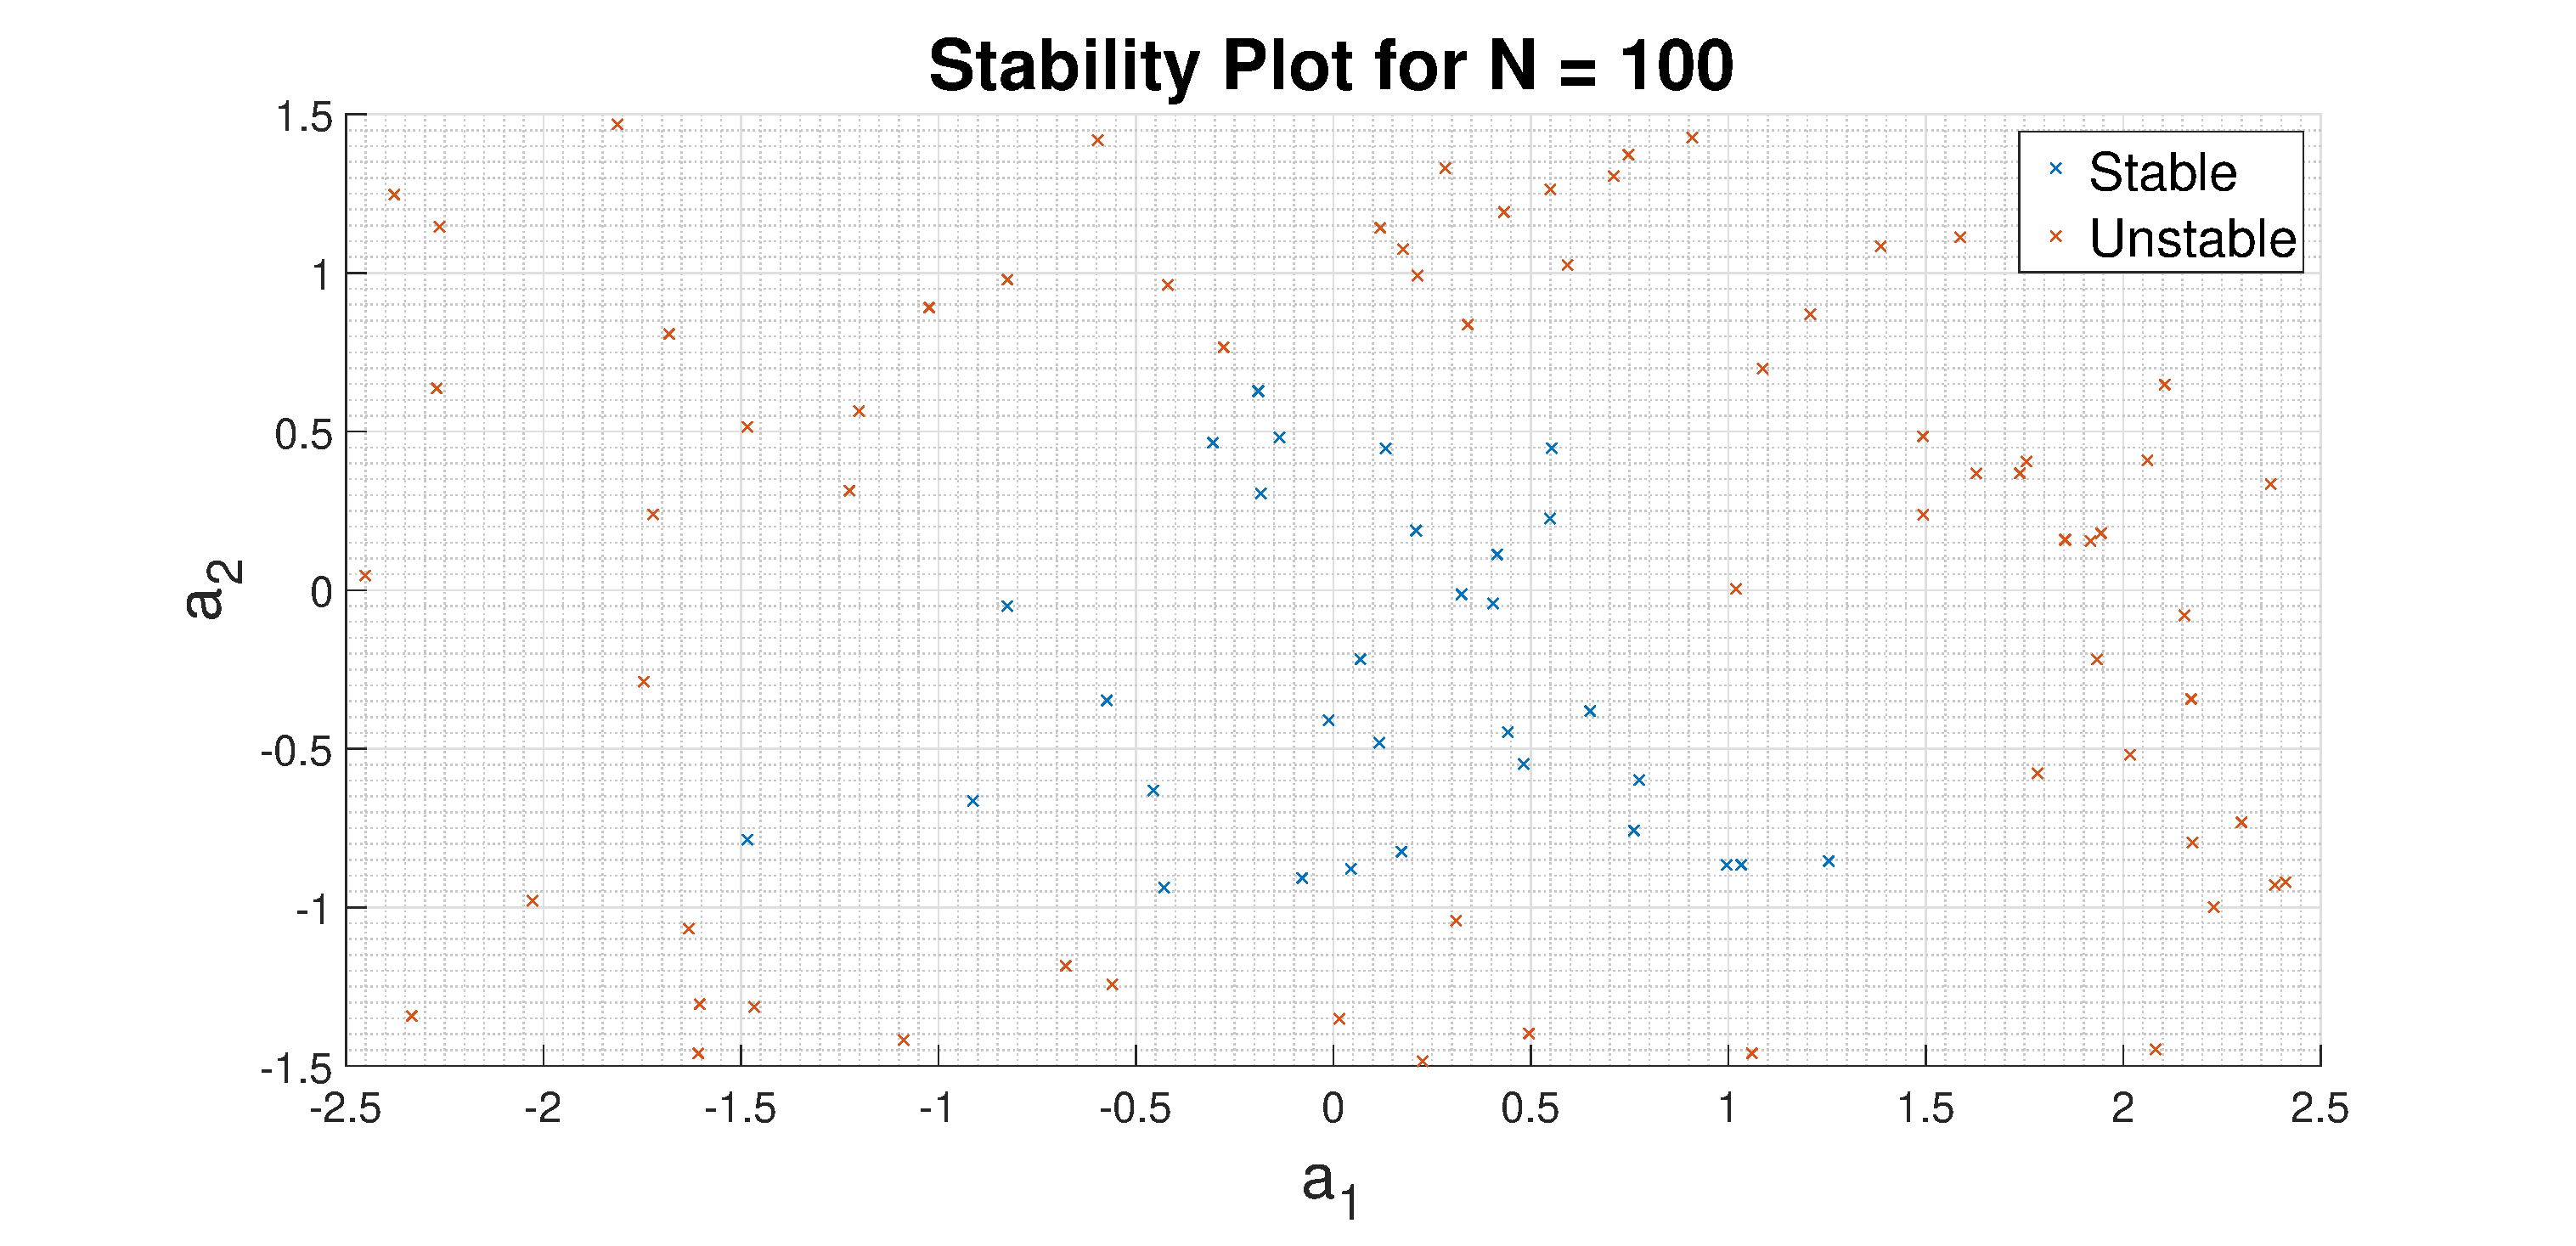
\includegraphics[width=0.49\textwidth]{stability_plot_n_100}
    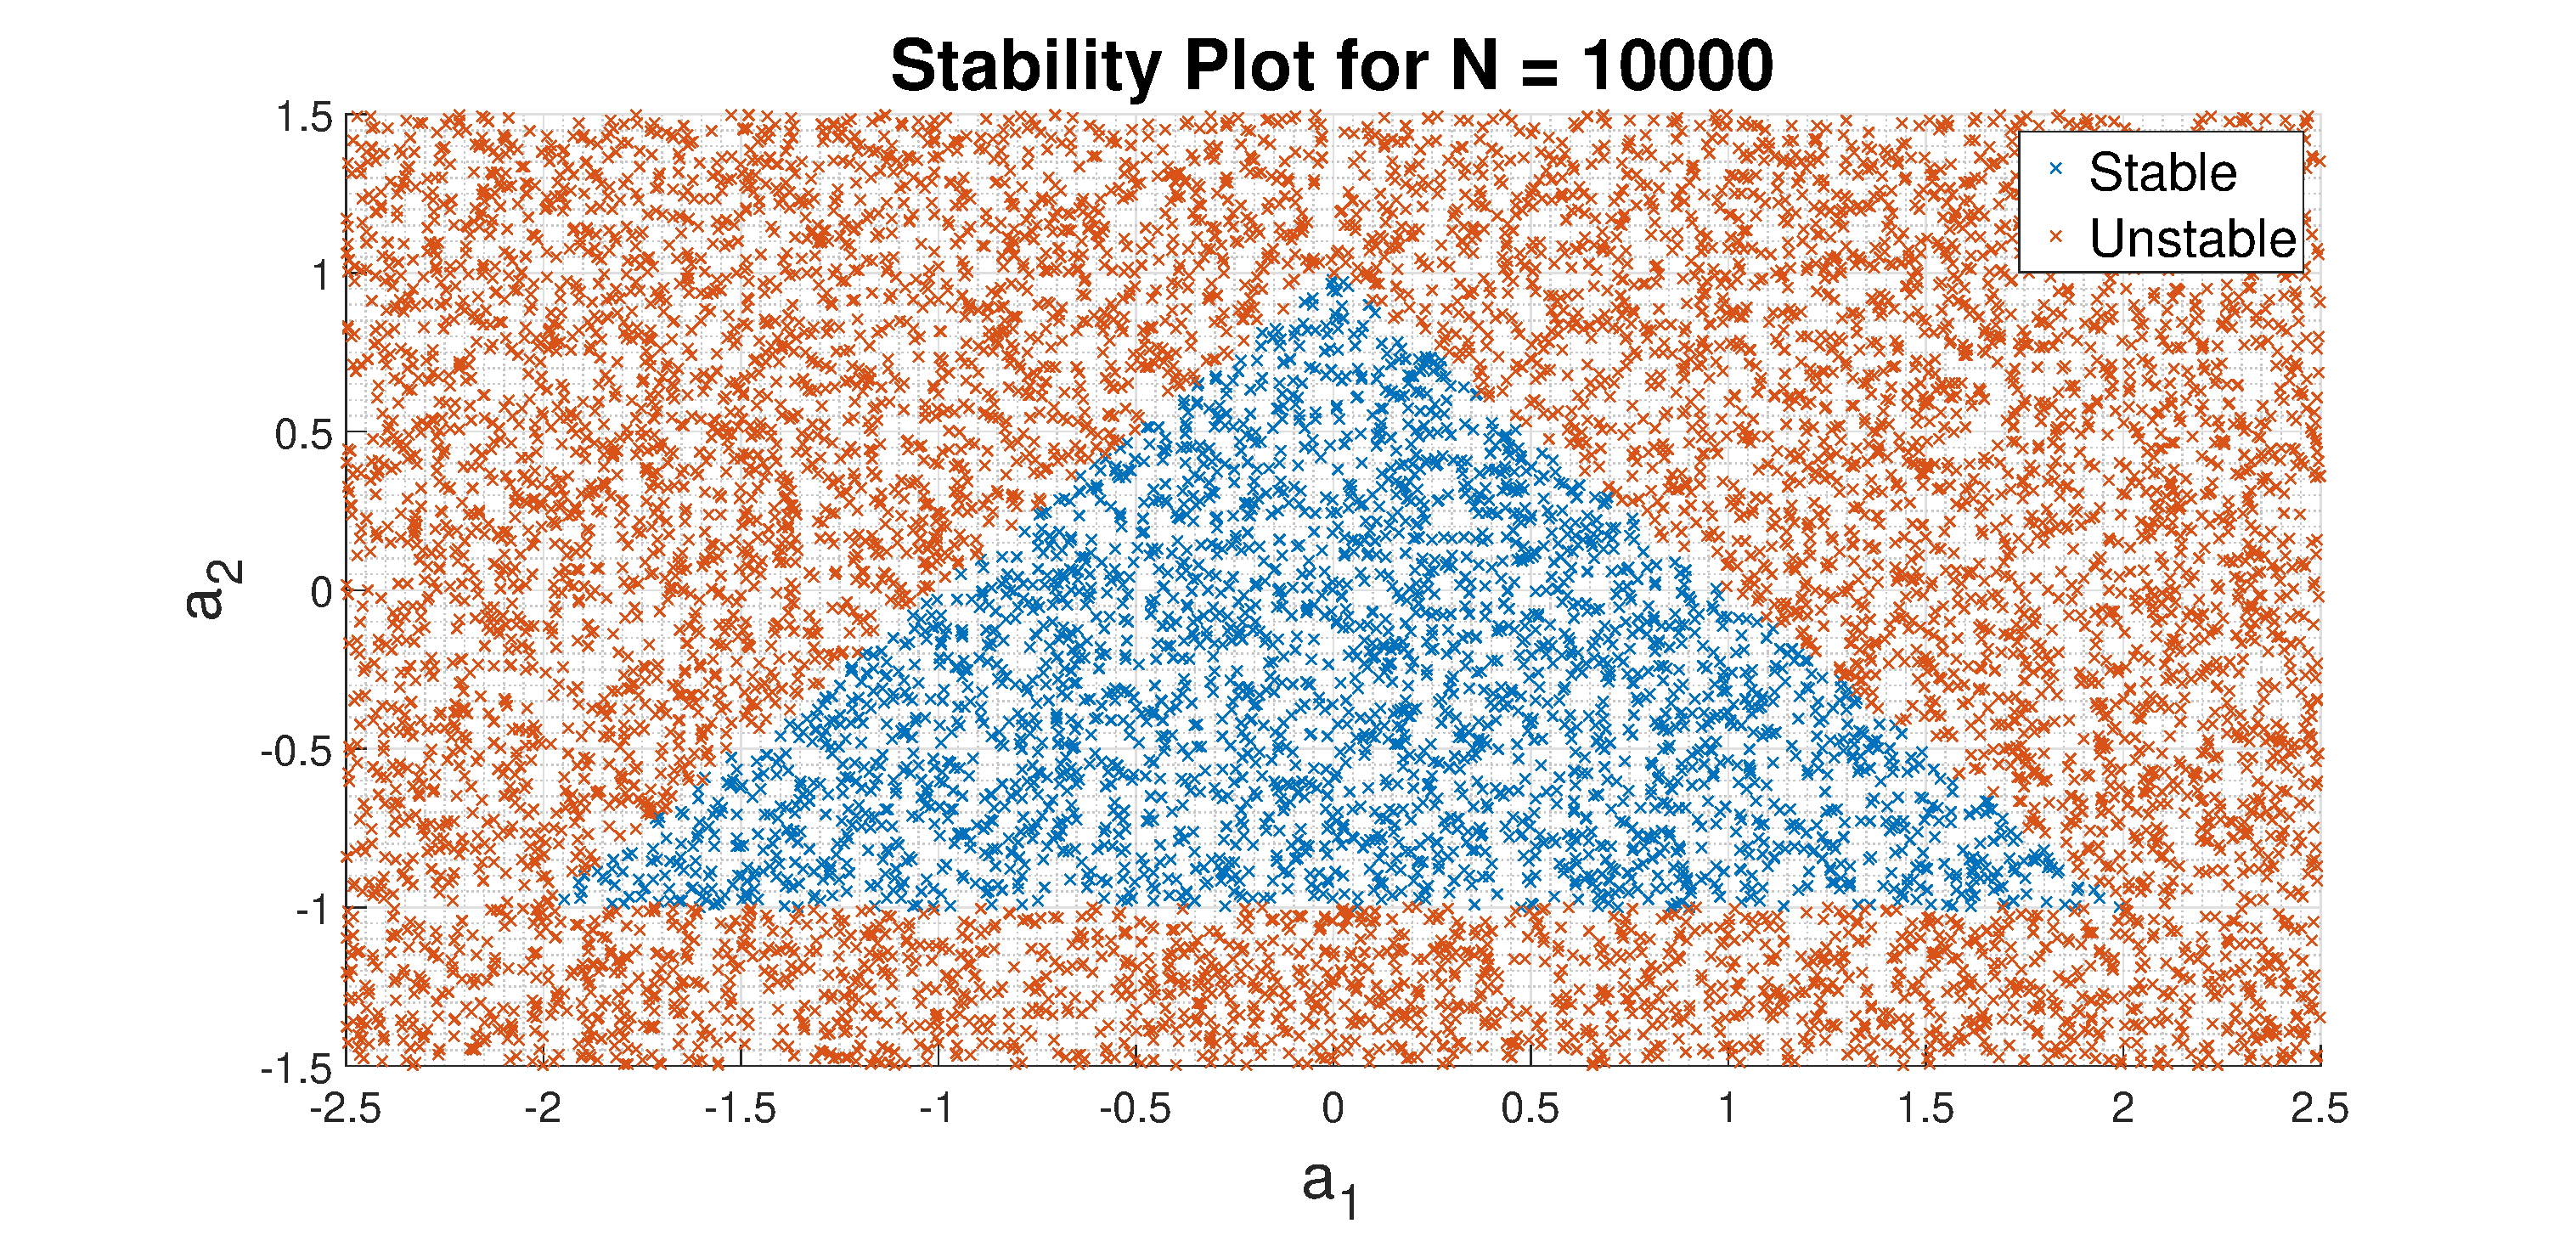
\includegraphics[width=0.49\textwidth]{stability_plot_n_10000}
    \caption{Stability plots for AR(2) process}
    \label{fig:AR_stability}
\end{figure}

The general form of an AR(2) process has been defined in the coursework handout. For the process to be stable, the three inequalities listed below have to be met.

\begin{align}
    a_{1} + a_{2} &< 1\nonumber\\
    a_{1} - a_{2} &< 1\nonumber\\
    |a_{2}| &< 1\nonumber
\end{align}

The three inequalities define a triangular region on the $a_{1}a_{2}$ plane. Within the defined region, the response of all AR(2) process will be bounded; they will be wide-sense stationary. Outside this region, the response of the processes will diverge; they will not be wide-sense stationary as the mean of the process is changing.\\

The inequalities listed above are obtained by noting that the process will only be stable if the poles of the system lie within the unit circle. To determine the position of the poles, the characteristic equation $C(z) = z^2 - a_{1}z - a_{2}$ is studied. The roots of the equation can be found using the equation $z = \nicefrac{a_1 + \sqrt{a_1^2+4a_2}}{2}$. If $a_{1} + 4a_{2} \geq 0$, the roots will be real. Otherwise the roots will be complex conjugates.\\

If the roots are real, the larger root has to be less than 1,

\begin{align}
   \frac{a_1 + \sqrt{a_1^2+4a_2}}{2} &< 1\nonumber\\
   a_1^2+4a_2 &< a_1^2-4a_1+4\nonumber\\
   a_1+a_2&<1
\end{align}

and the smaller root has to be greater than -1,

\begin{align}
   \frac{a_1 - \sqrt{a_1^2+4a_2}}{2} &> -1\nonumber\\
   a_1^2-\sqrt{a_{1}^2+4a_{2}}&< -2\nonumber\\
   a_2-a_1&<1
\end{align}

Lastly, if the process has 2 real roots then the characteristic equation can be expressed as, $C(z) = (z-\lambda_1)(z-\lambda_2)=0$. Expanding, we get $C(z) = z^{2} - (\lambda_{1}+\lambda_{2})z +\lambda_1\lambda_2 = 0$. For the random process to be stationary, $|\lambda_{1}|<1$ for $i=1,2$. Thus, $a_{1}=(\lambda_{1}+\lambda_{2})$ and $a_{2} = \lambda_1\lambda_2$. Since $|\lambda_i|<1$, $|a_{2}|<1$.



\begin{figure}[H]
    \centering
    \includegraphics[width = 0.49\textwidth]{acf_sunspot_n_5}
    \includegraphics[width = 0.49\textwidth]{acf_sunspot_n_20}
    \caption{ACF of sunspot time series for data lengths N=5 and N=20}
    \label{fig:acf_sunspot_1}
\end{figure}

2. The ACF of the sunspot time series is graphed for data lengths of 5 and 20 in figure \ref{fig:acf_sunspot_1}. With data length N=5, trends cannot be clearly observed; a longer data series is required. When data length N=20, a sinusoidal trend starts to appear. 

\begin{figure}[H]
    \centering
    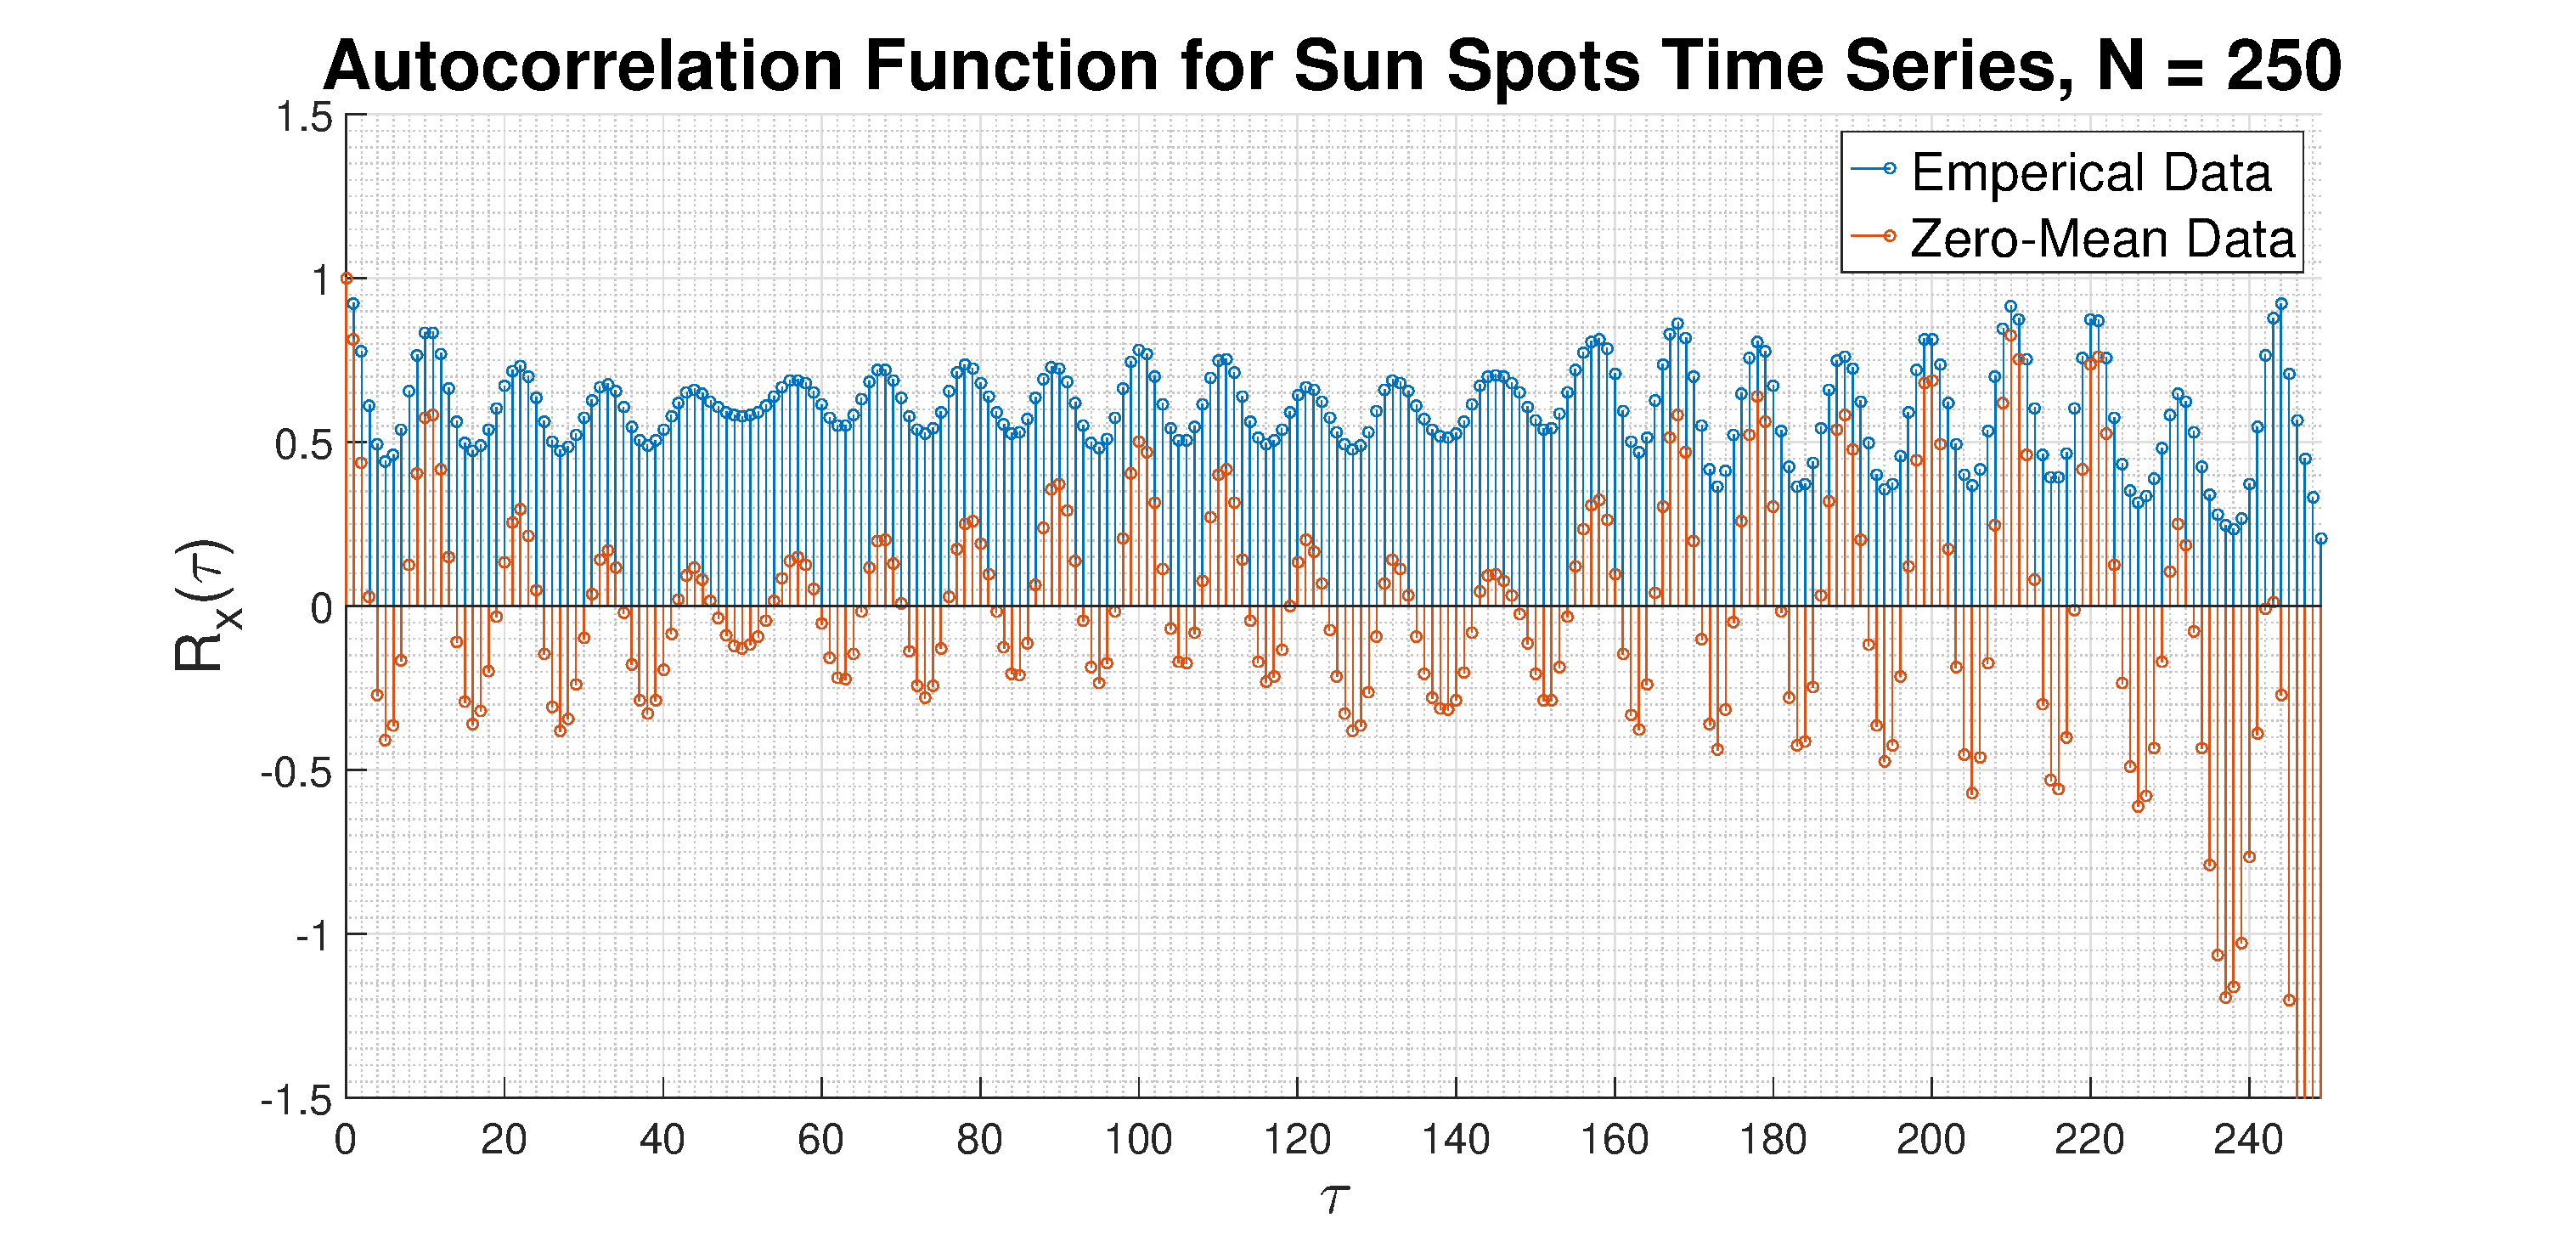
\includegraphics[width = 0.49\textwidth]{acf_sunspot_n_250}
    \includegraphics[width = 0.49\textwidth]{acf_sunspot_n_250_zoom}
    \caption{ACF of sunspot time series for data length N=250}
    \label{fig:acf_sunspot_2}
\end{figure}

With data length N=250, the best sinusoidal trend is observed. The ACF is not a perfect sinusoid and irregularities occur at $\tau$=50 and $\tau=$100. These irregularities are most likely due to the fact that the data length is N=250. An empirical bound was placed on the ACF function in section \ref{sec:acf_uncorrelated} beyond which the estimate of the ACF becomes unreliable. The empirical bound stated above was $\nicefrac{N}{10}$; as such, the ACF function should only be studied for $\tau < 25$. Figure \ref{fig:acf_sunspot_2} shows a zoom of the ACF of the zero-mean sunspot series for N=250. In this region, the ACF resembles the shape of the ACF of an AR(2) system with $a_{1}>0$ and $a_{2}<0$. Lastly, the bias inherent in the empirical data hides trends that can be easily observed with the zero-mean data.\\

\begin{figure}[H]
    \centering
    \includegraphics[width = 0.49\textwidth]{par_corr_sunspot}
    \caption{PACF for sunspot time series}
    \label{fig:par_corr_sunspot}
\end{figure}


3. The partial autocorrelation function (PACF) of the sunspot time series is graphed in figure \ref{fig:par_corr_sunspot}. It is important to note that the standardised plot yields a result that is slightly different from the empirical data. Using zero-mean unit-variance data removes all biases and thus produces a more accurate answer. Ideally, the PACF should be 0 for $\tau > p$, where $p$ is the model order; however for real data, a small threshold has to be introduced. As seen in the graph, the threshold has been set to 0.2. It is evident that the PACF function decreases significantly after order 2. This suggests that the current sample at any point in time is not strongly correlated to the sample three time instances ago. The PACF correlation function corroborates the findings above; it is most likely that sunspot time series is an AR(2) process.\\ 

4. The Minimum Description Length (MDL) and the Akaike Information Criterion (AIC) introduce a "penalty" for overestimating the order number. Both criteria were first introduced in the field of information theory; the main motivation behind the criteria is to balance the trade-off between the error incurred and the computational complexity involved in utilising a certain model. In practice, increasing the order of the model almost always reduces the error and thus a penalty is needed to limit the order number; without this penalty, a higher model order will usually be preferred. \\ 

\begin{figure}[H]
    \centering
    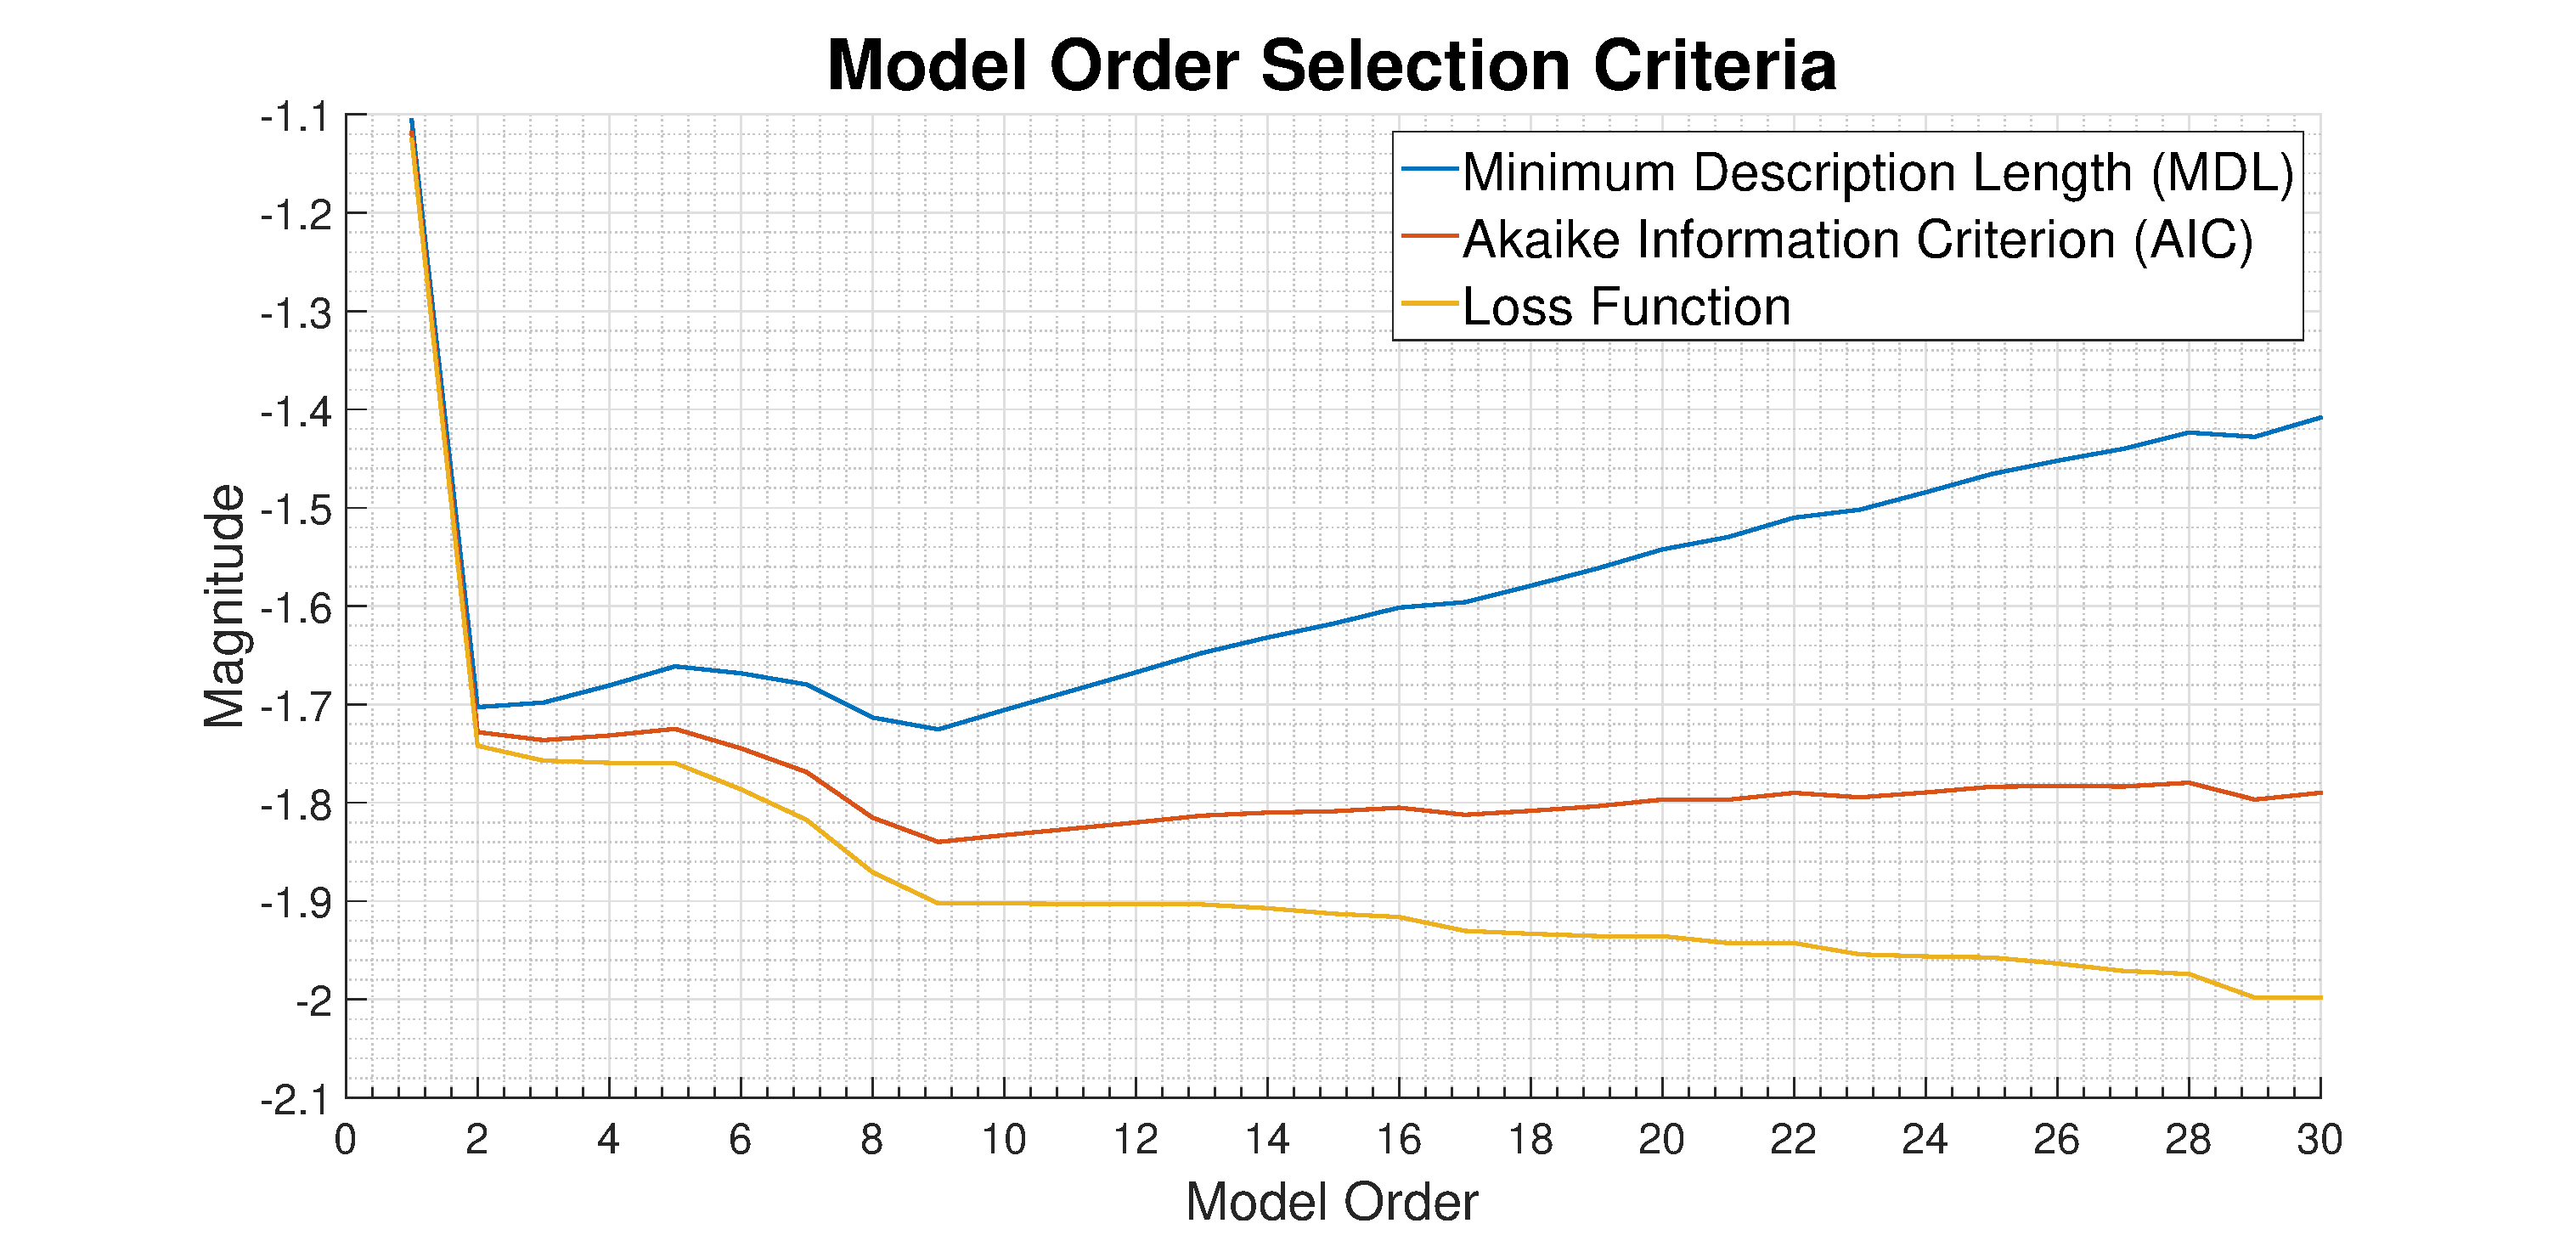
\includegraphics[width = 0.49\textwidth]{MLD_AIC_loss_sunspot}
    \caption{Model selection creteria for sunspot time series: MLD, AIC, Loss Function}
    \label{fig:MLD_AIC_loss_sunspot}
\end{figure}

Figure \ref{fig:MLD_AIC_loss_sunspot} shows the MDL, AIC and the loss function for the sunspot time series. Note that the loss function is calculated by taking the log of the estimated variance as calculated by the {\tt aryule} function. The estimated variance is a scaled version of the cumulative squared error, where the scaling factor is the length of the time series. The loss function confirms the assertion made above; increasing the order of the estimated model decreases the error. However, an optimal model is one that minimise the MDL and AIC function. Based on that criteria, it is clear that the sunspot time series should be modelled as either an AR(2) or an AR(9) process.\\ 

It should be noted that over-modelling can lead to spectral line splitting. While this may reduced the error incurred, the model will not be representative of real data. As such, the sunspot time series should be modelled as an AR(2) process.\\

5. Using the AR models calculated above, future values of the sunspot time series can be predicted. The MATLAB function {\tt predict} is used and the results obtained for different combinations of model orders and prediction horizons have been graphed in figure \ref{fig:ar_prediction_1}.

\begin{figure}[H]
    \centering
    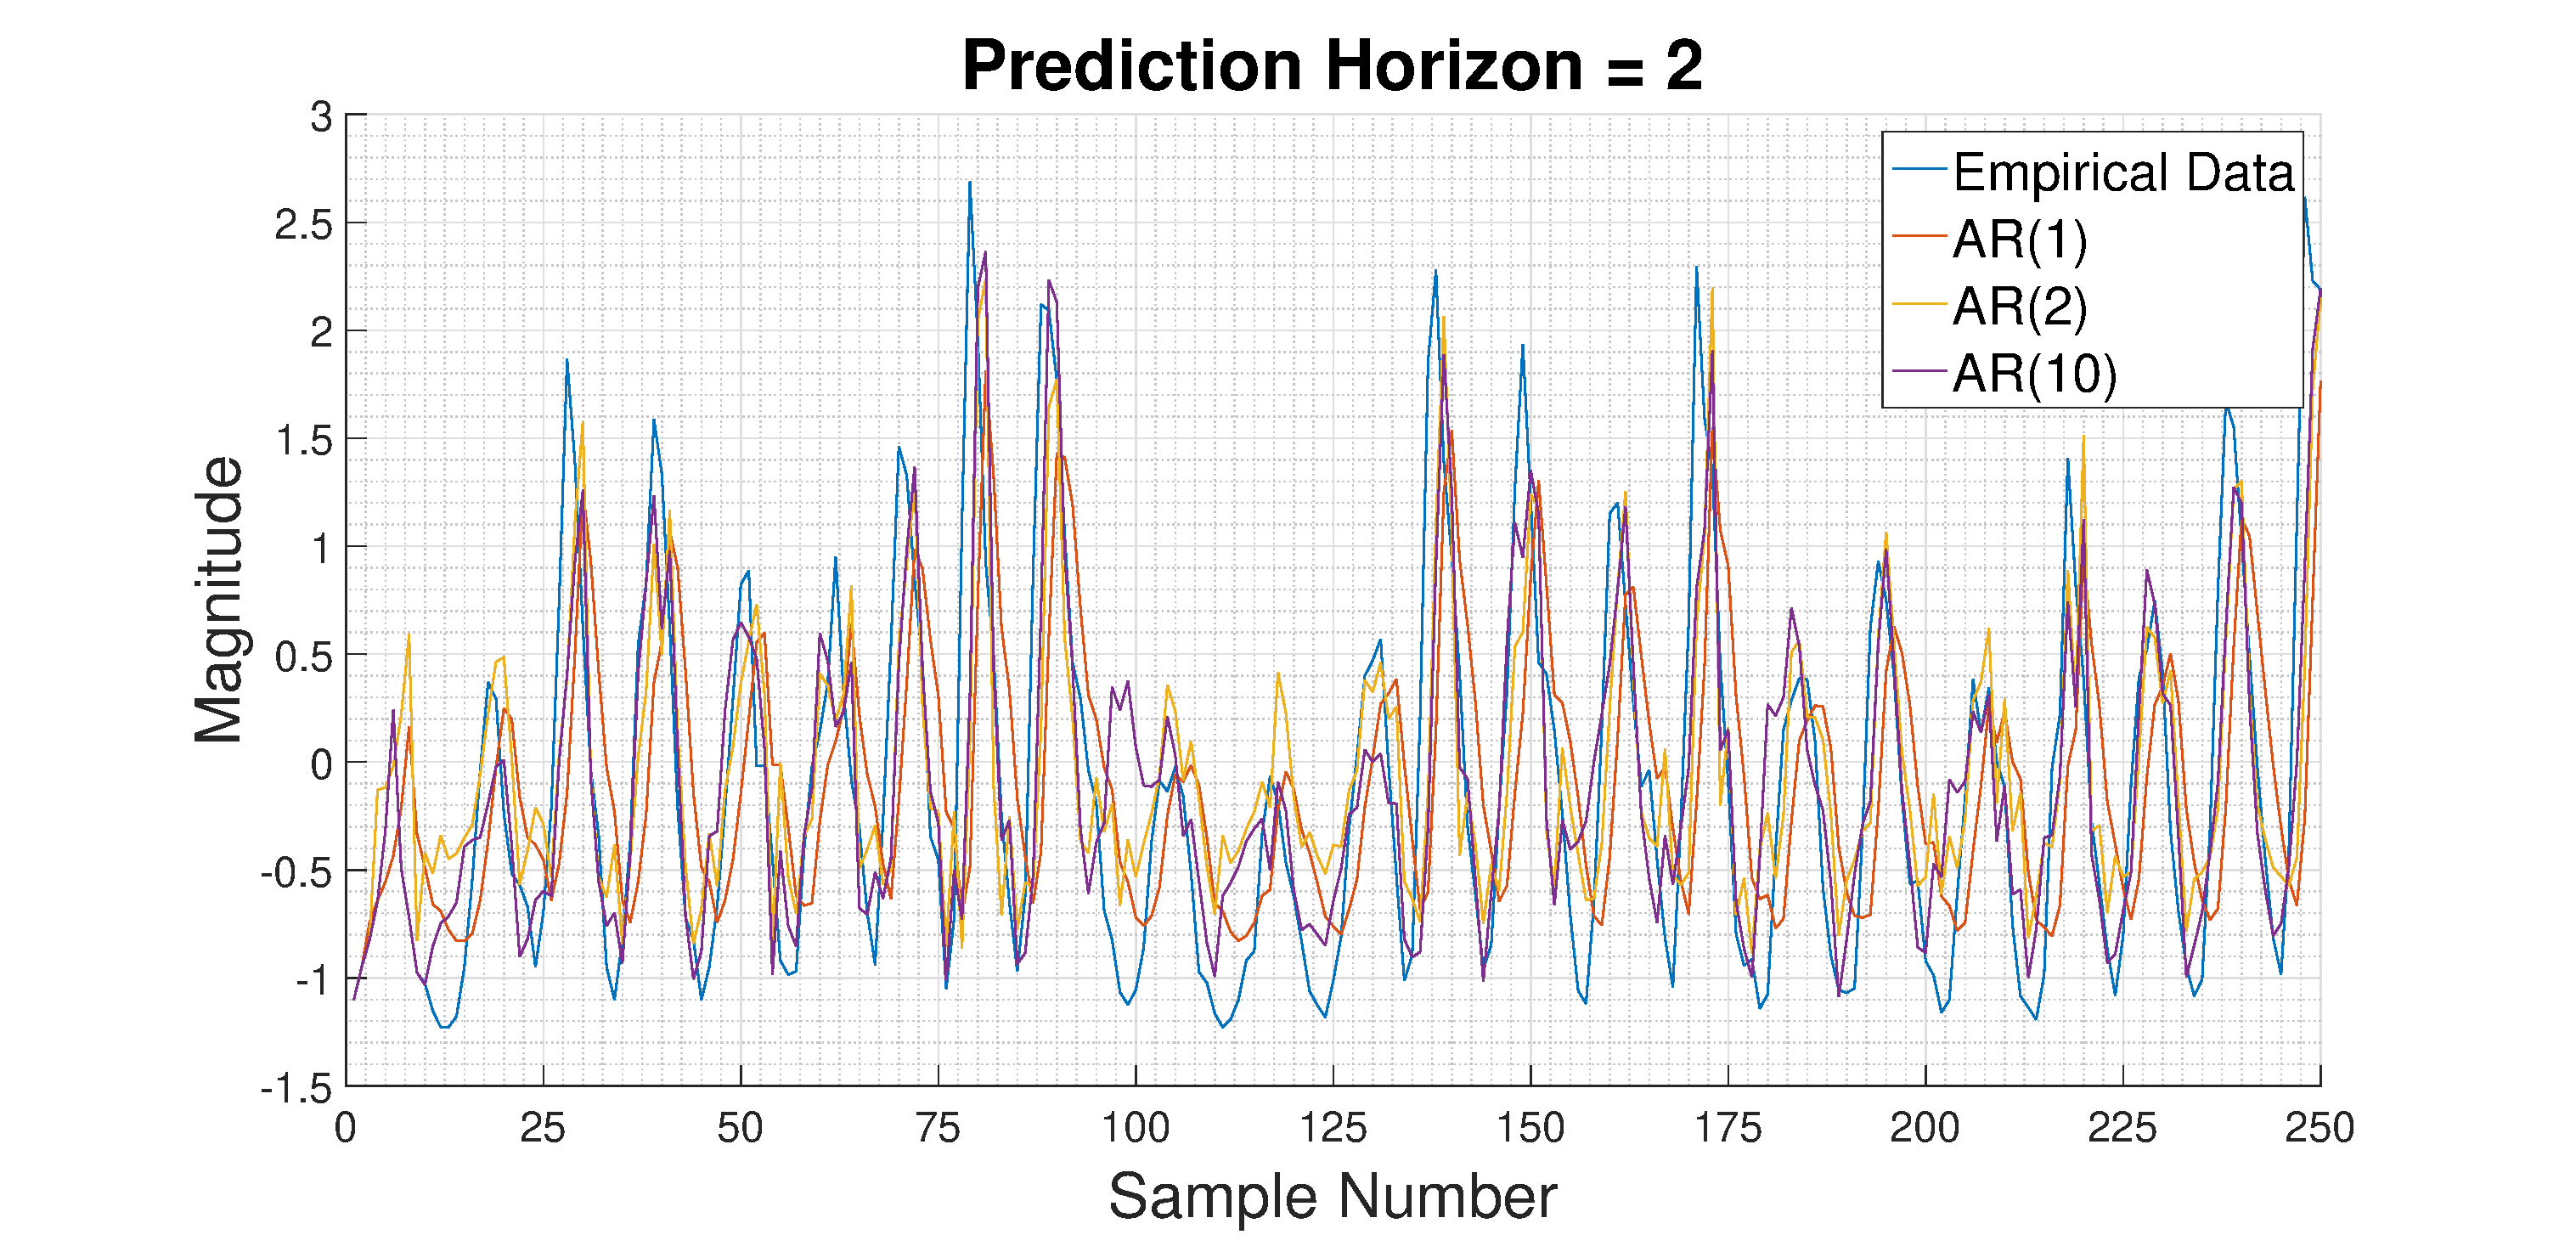
\includegraphics[width = 0.49\textwidth]{sunspot_prediction_horizon_2}
    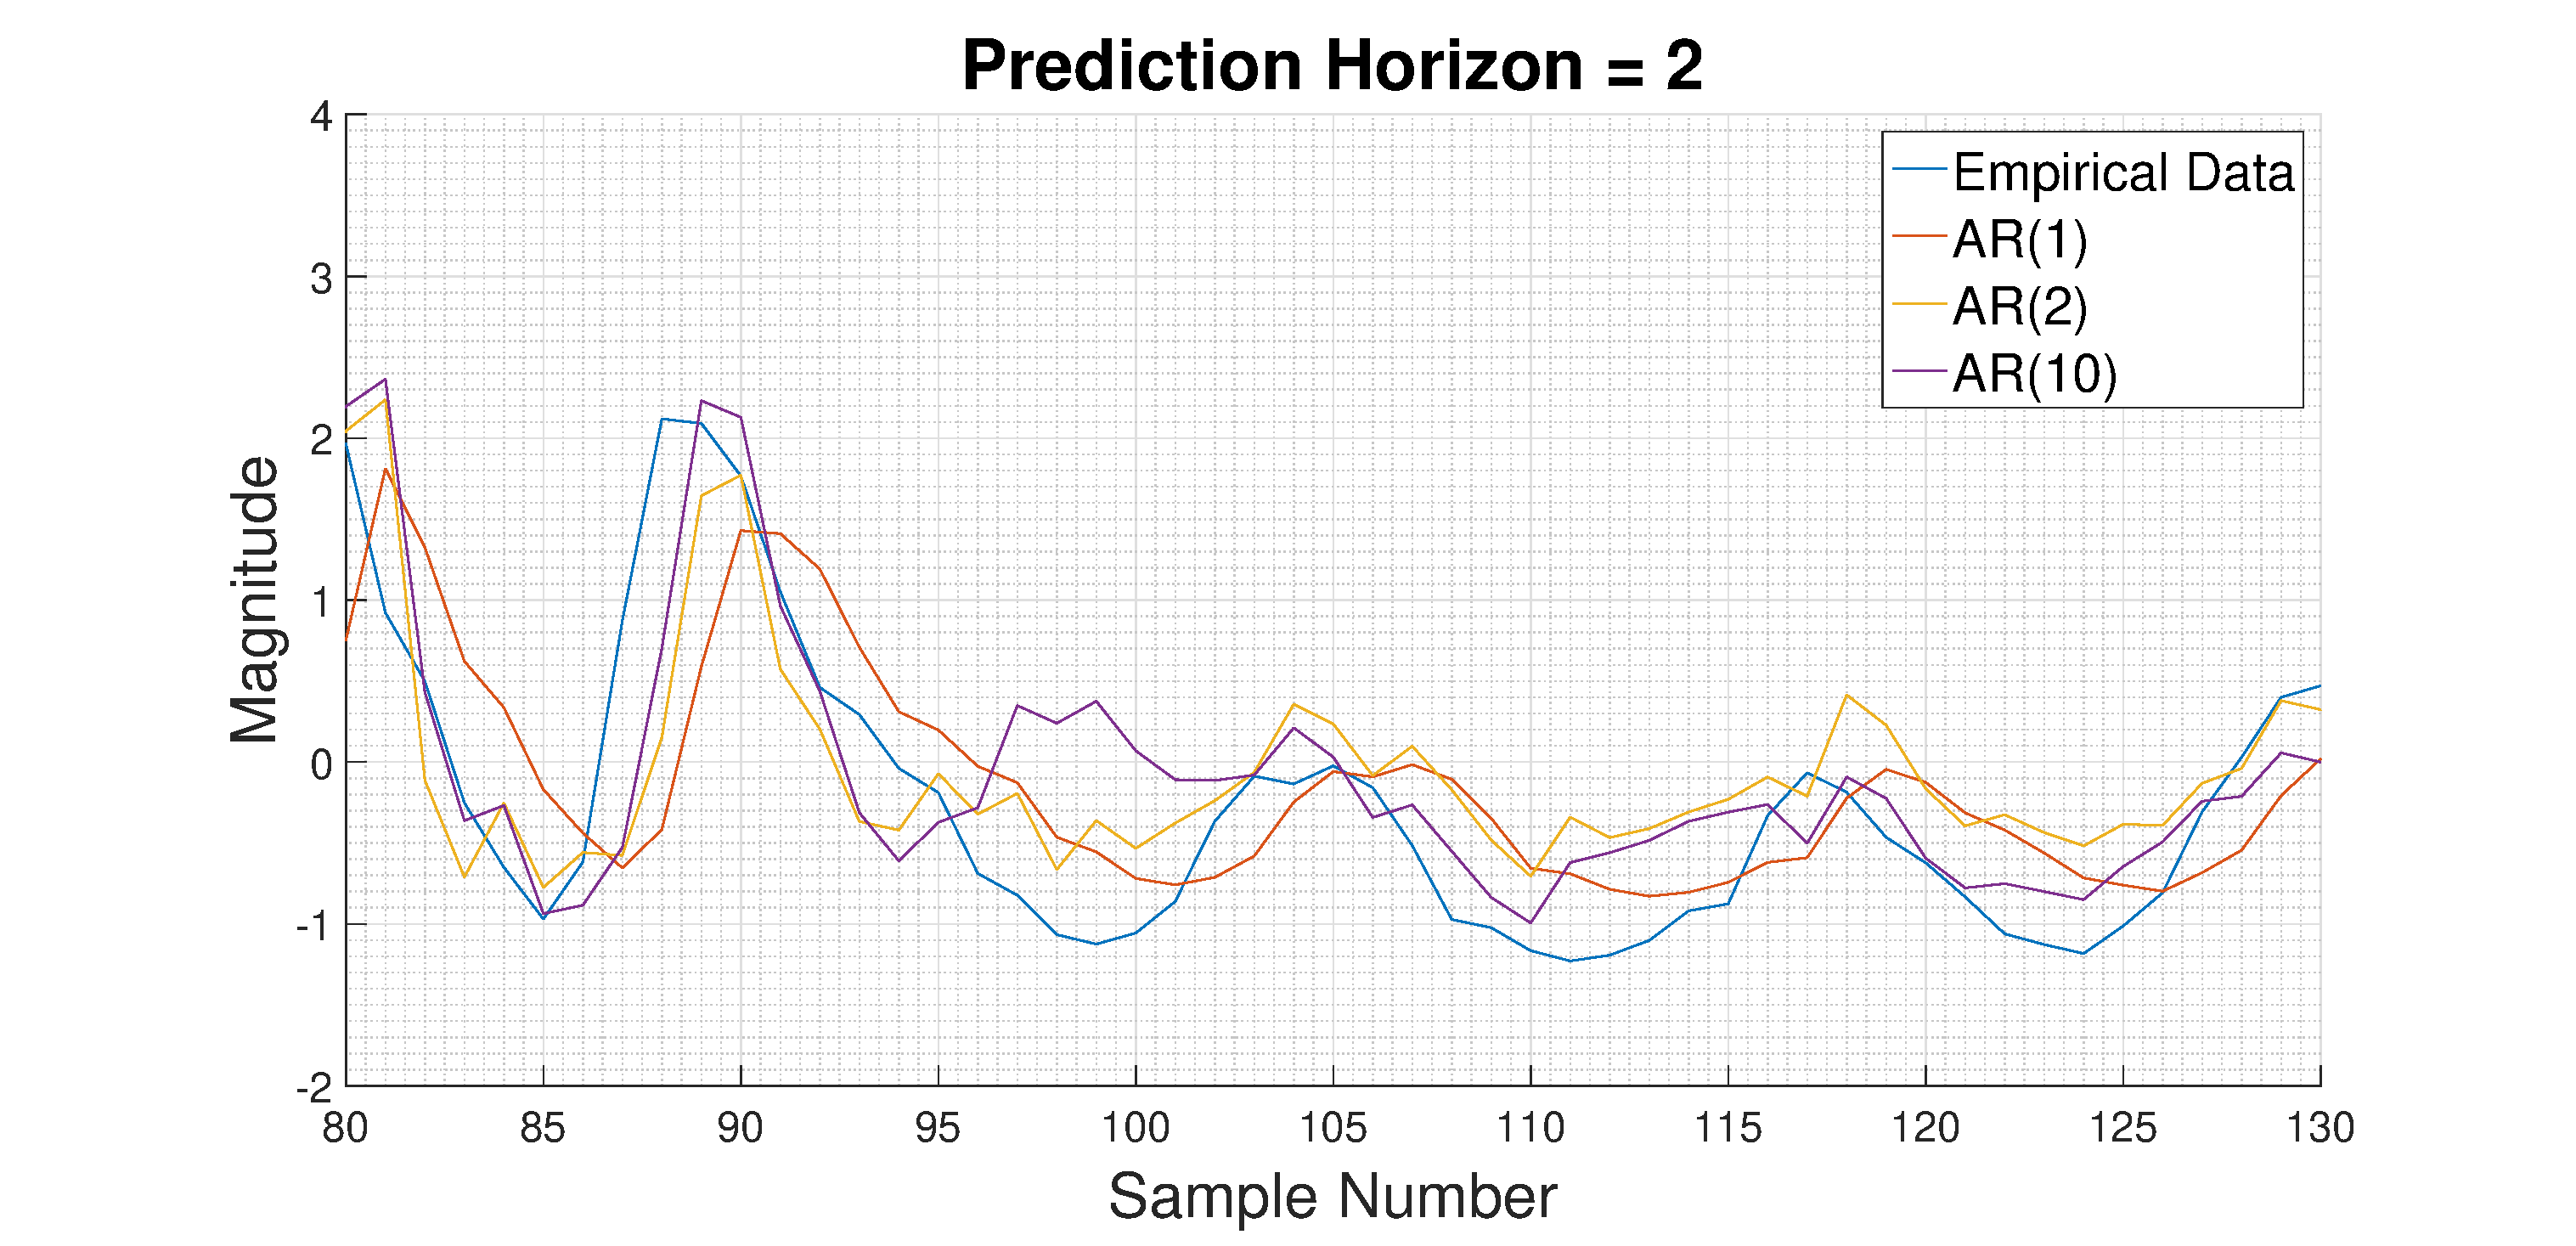
\includegraphics[width = 0.49\textwidth]{sunspot_prediction_horizon_2_zoom}
    \caption{Sunspot time series prediction: horizon = 2}
    \label{fig:ar_prediction_1}
\end{figure}

From figure \ref{fig:ar_prediction_1}, the first thing to notice is that using the AR(1) model, the prediction seems to be lagging the real data. The AR(1) model provides too few degrees of freedom to correctly represent the data. The current sample seems to depend on more that just the previous sample. Observe the prediction made using the AR(2) model; the lag has been reduced. Both the AR(1) and AR(2) model seem to be reacting to changes rather than exploiting the periodic nature of the sunspot series. The AR(10) model seems to predict peaks in the time series before they occur. This is evident near sample number 95. There is actually a dip in the number of sunspots however the AR(10) model predicts a peak. The AR(1) and AR(2) models predicted the trough well.\\

From figure \ref{fig:ar_prediction_2}, it is clear that using a small model order yields bad predictions for large horizons; using AR(1) and AR(2) and predicting 10 years into the future, little information about the number of sunspots can be obtained. Although the peaks in the predicted data correspond strongly to the peaks the empirical data, the amplitude of the prediction is significantly lower. The decrease in amplitude of the prediction as the prediction horizon increases is a trend that can be observed across all three models.

\begin{figure}[H]
    \centering
    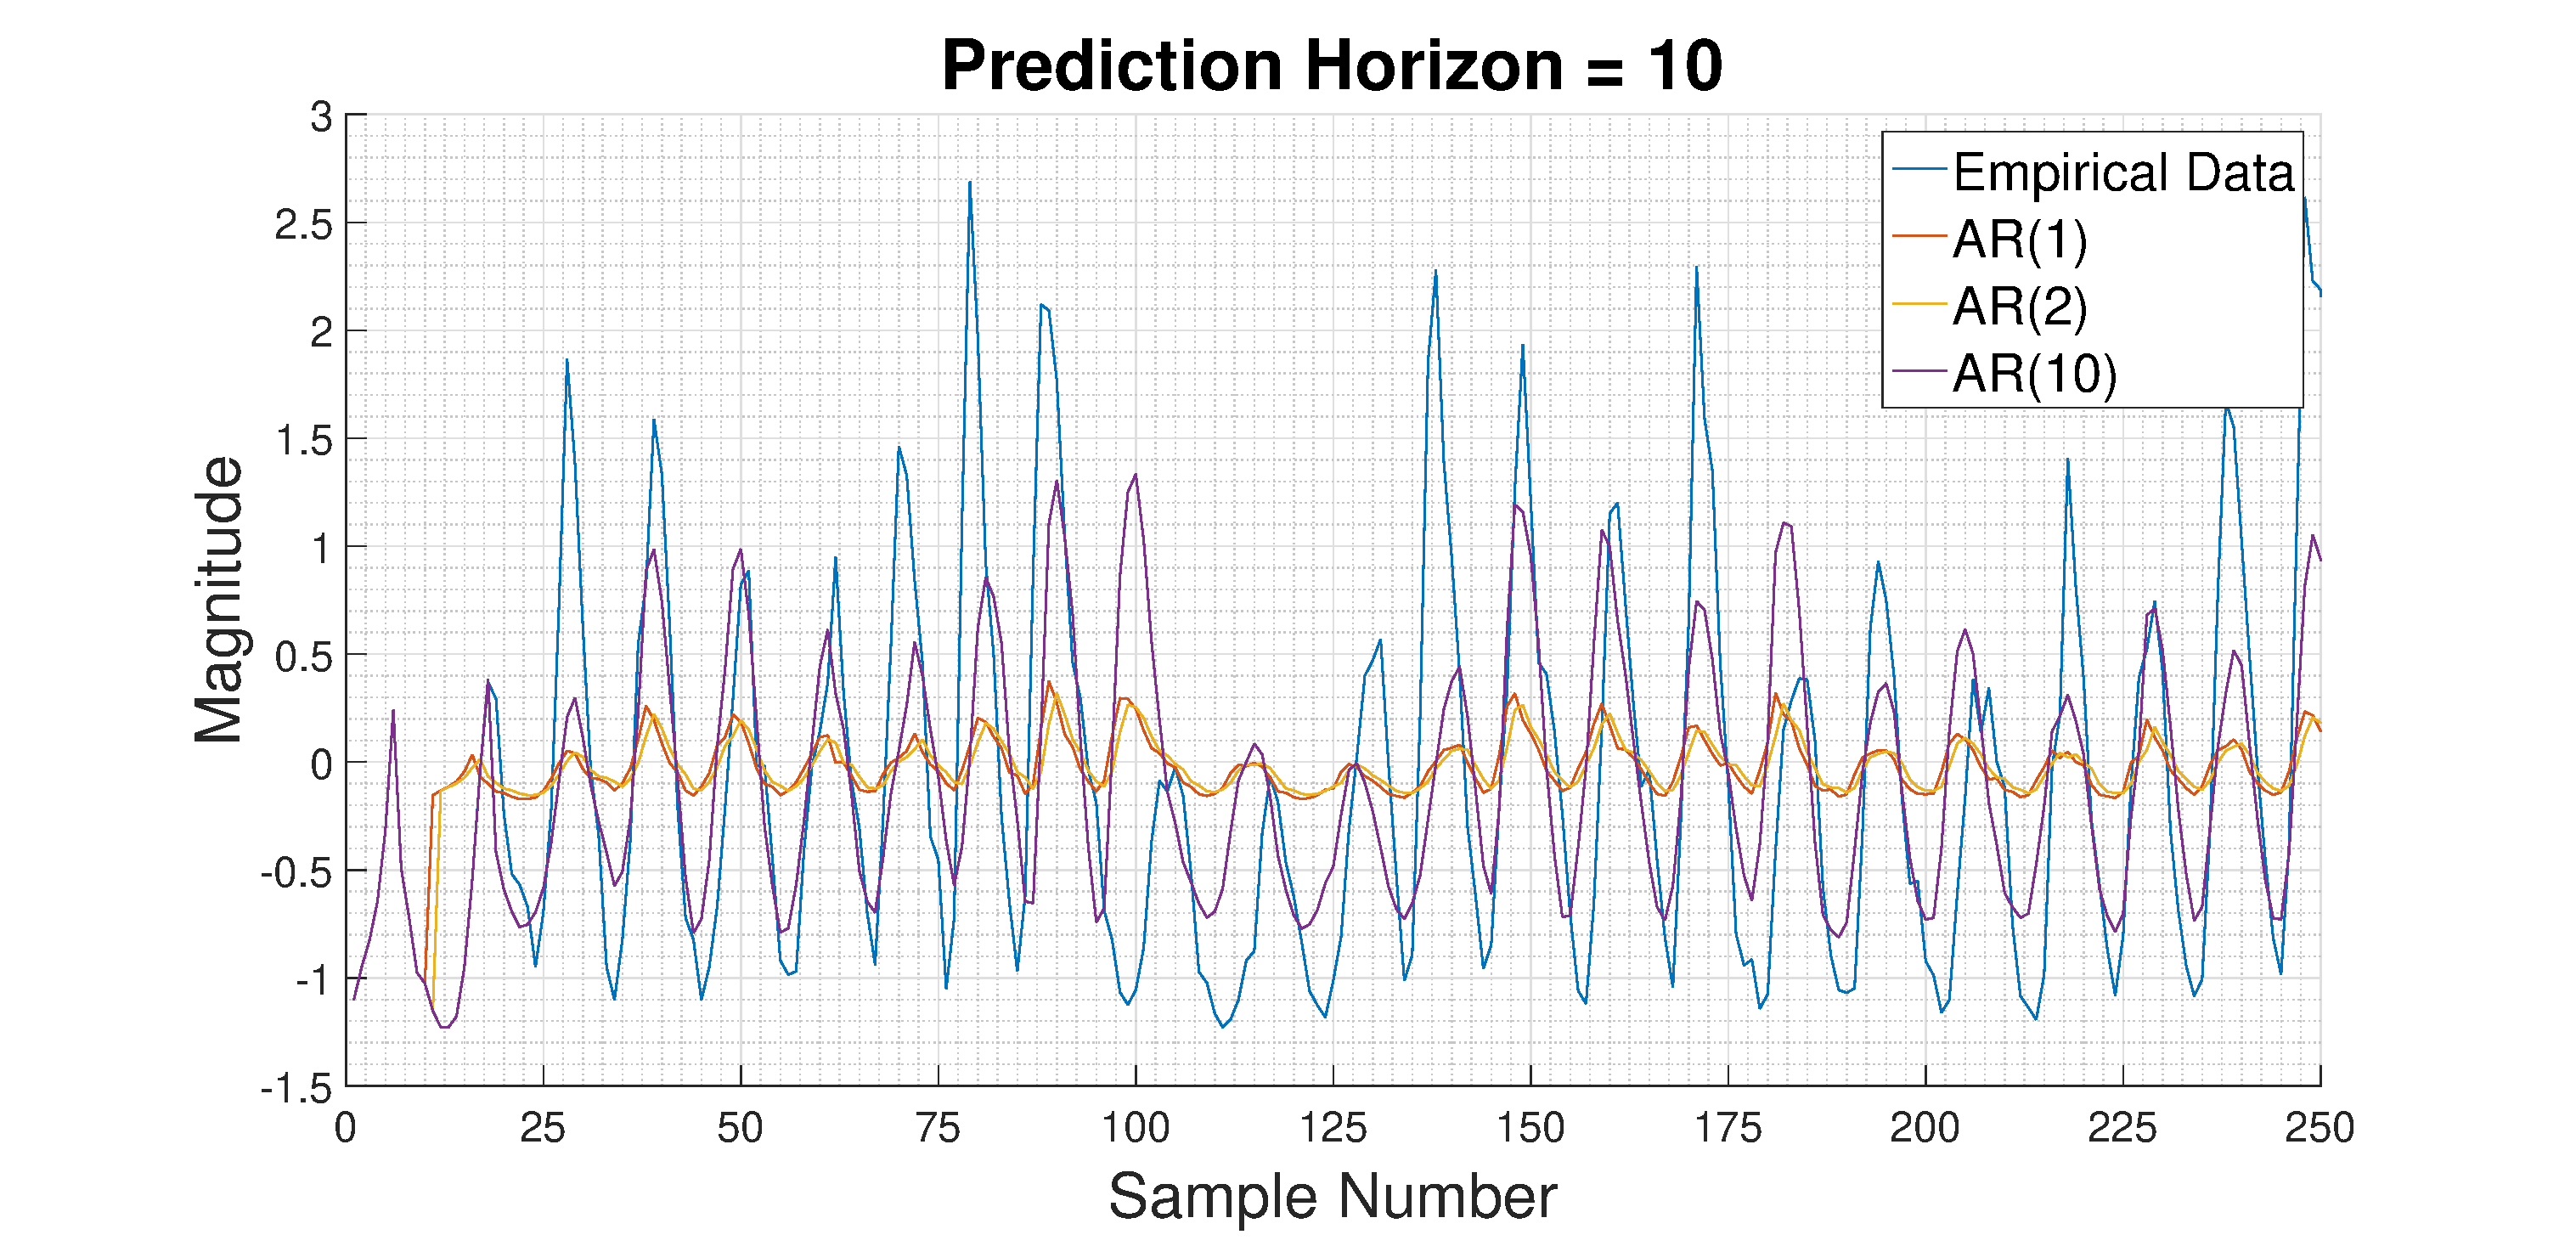
\includegraphics[width = 0.49\textwidth]{sunspot_prediction_horizon_10}
    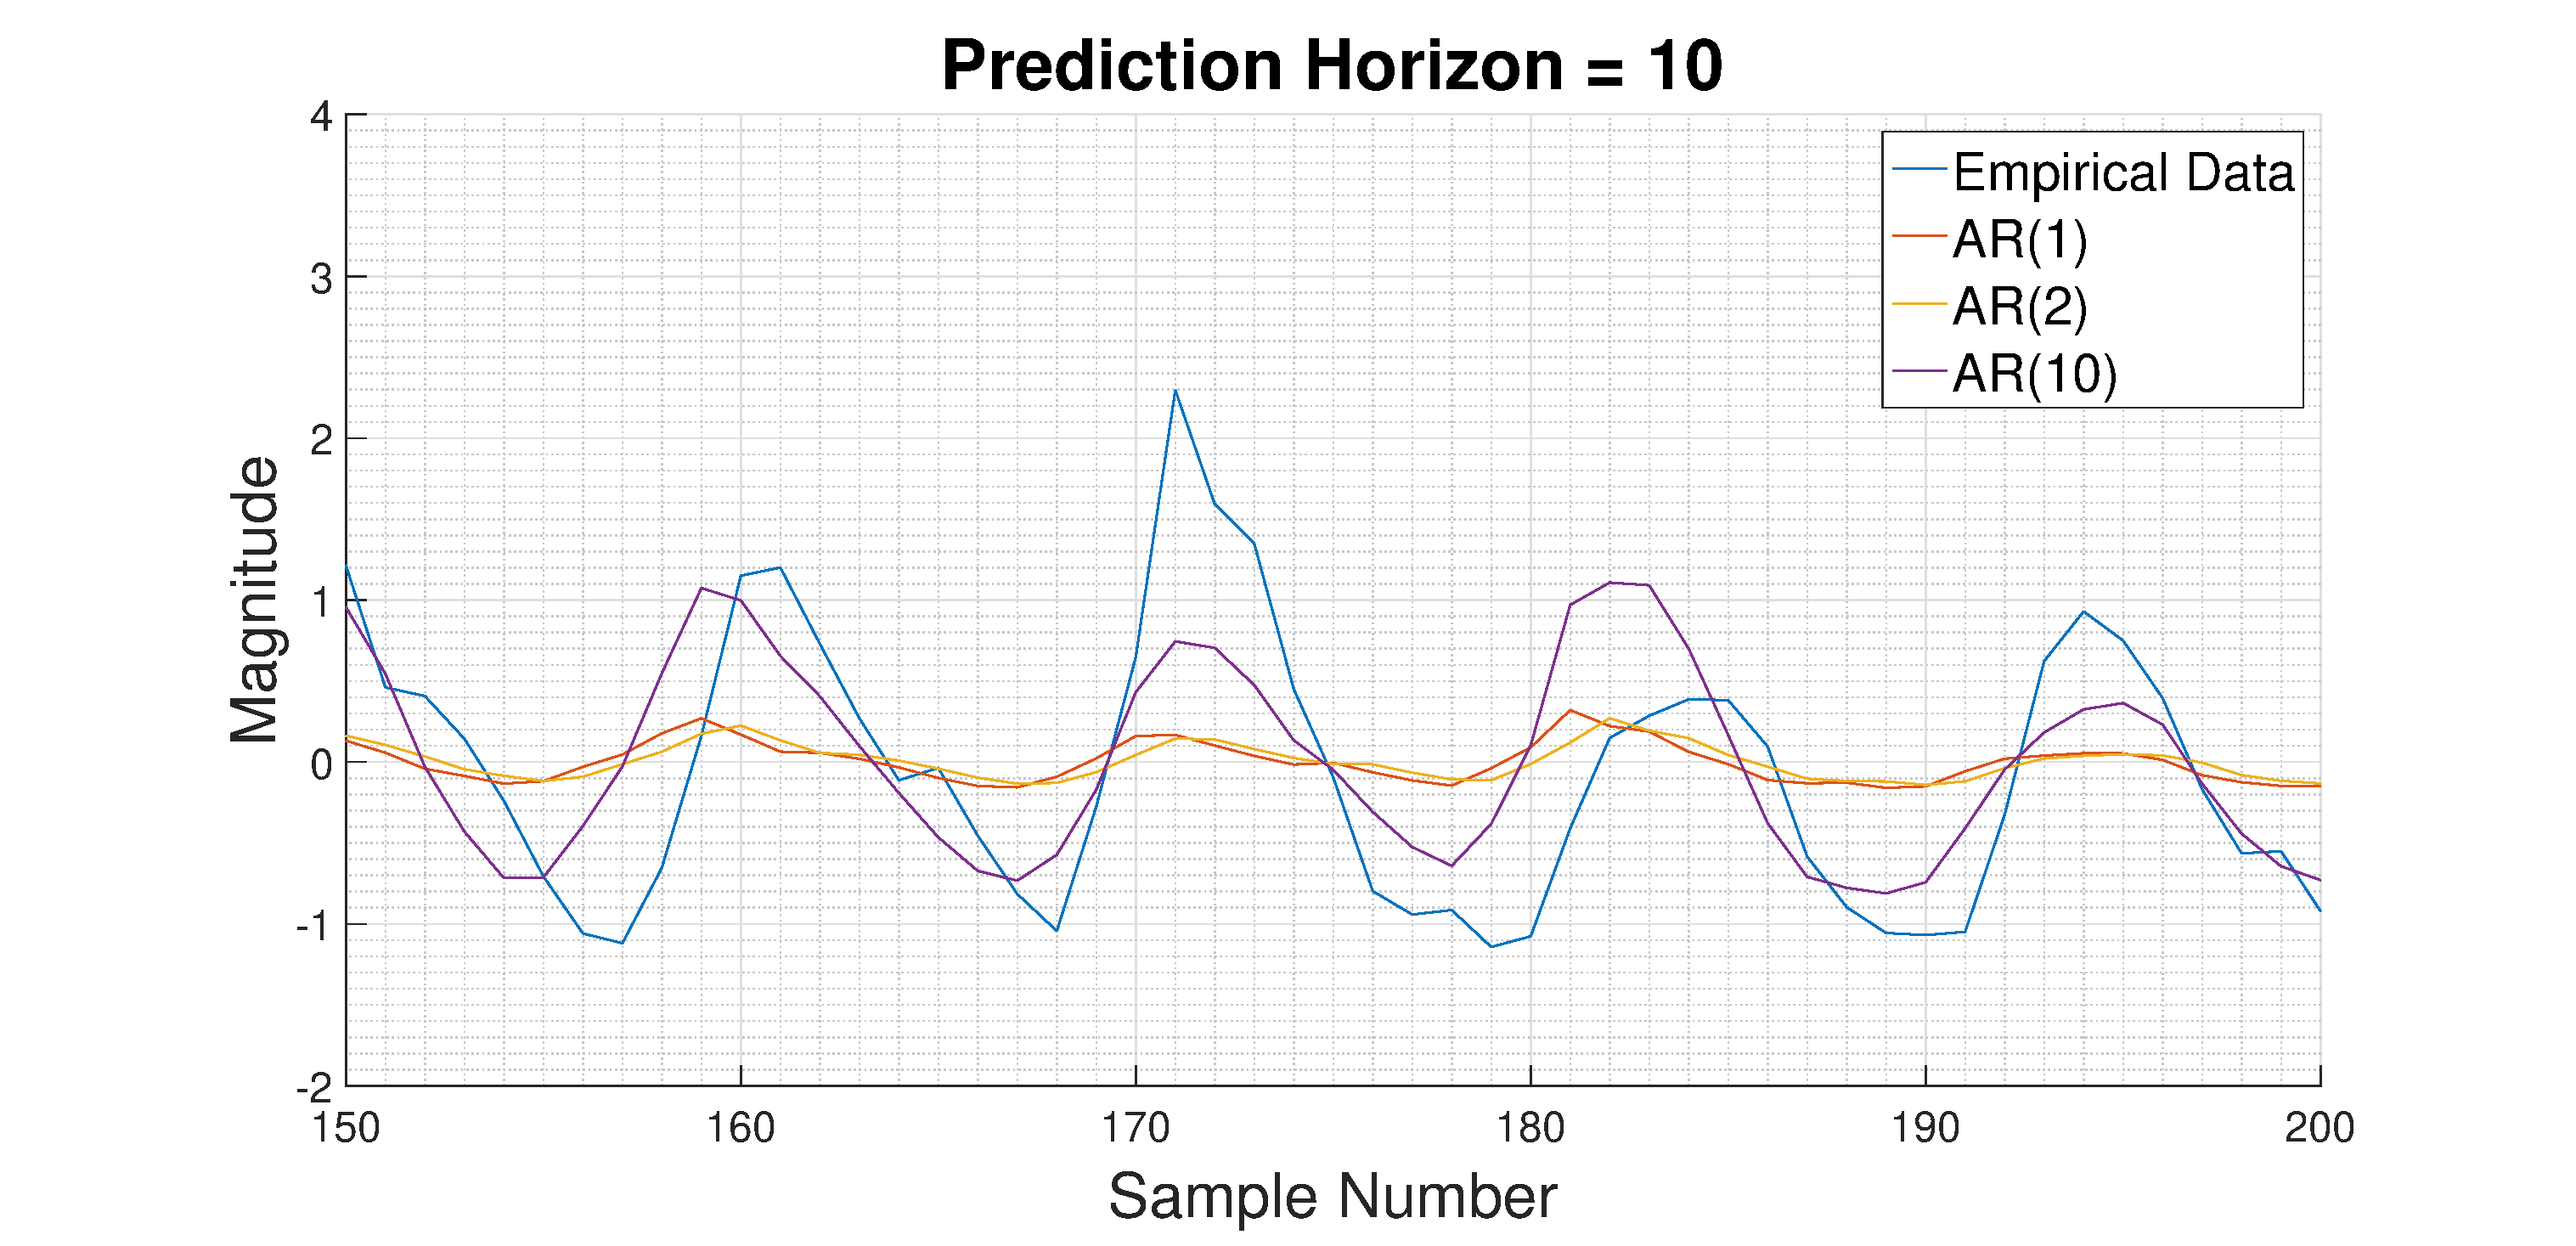
\includegraphics[width = 0.49\textwidth]{sunspot_prediction_horizon_10_zoom}
    \caption{Sunspot time series prediction: horizon = 10}
    \label{fig:ar_prediction_2}
\end{figure}


In both figure \ref{fig:ar_prediction_1} and \ref{fig:ar_prediction_2}, the expected value of the process has been graphed. When the expectation is taken, the input AWGN goes to zero. As such, it is equivalent to studying a process in which the input has been suddenly removed. Analysing such systems is a very involved process; careful analysis of the AR coefficients is required \cite{mandic}. For the sunspot time series, it is clear that if the input is cut, the system will gradually approach zero. Using an AR(10) model to predict 10 years into the future, the decrease in amplitude is not that significant. As such, it is intuitive to conclude that a large model order allows better prediction for long horizons.\\

Figure \ref{fig:ar_prediction_3} shows the results obtained when predictions are made for horizons 1 and 5. The observations corroborate the findings listed above. For a prediction horizon of 5, the AR(1) and AR(2) model provide invalid data whereas the AR(10) model provides somewhat reliable data. Again, it can be concluded that using a small order model to predict for large horizons produces inaccurate results. For a prediction horizon of 1, all models produce similar results. 


\begin{figure}[H]
    \centering
    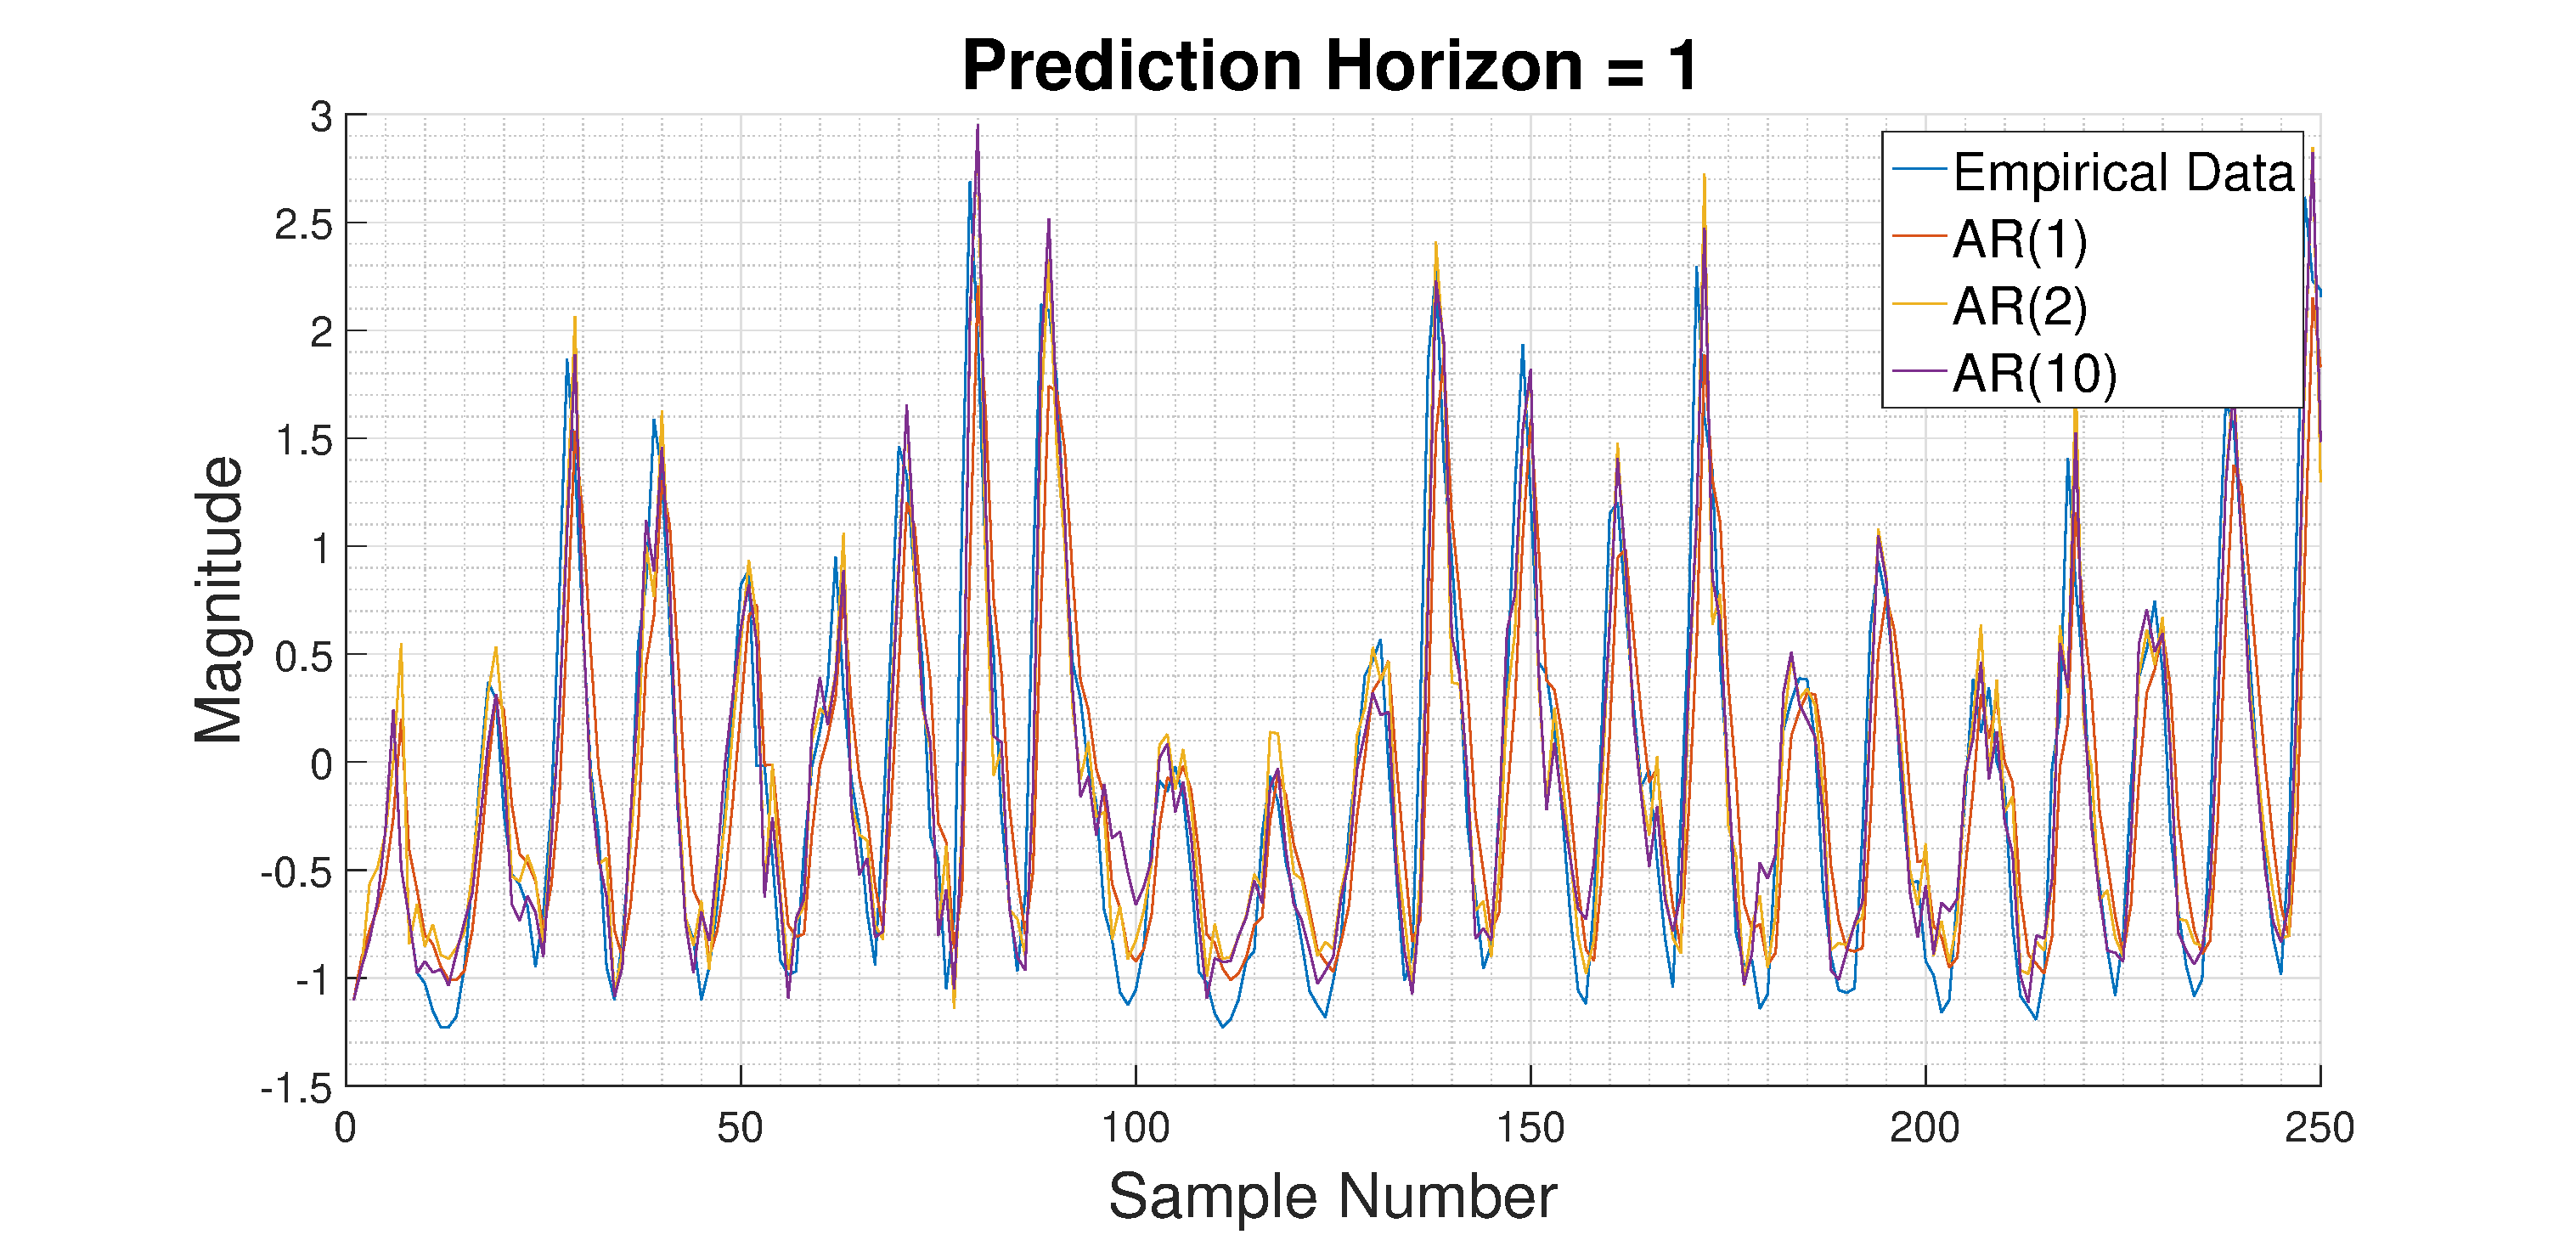
\includegraphics[width = 0.49\textwidth]{sunspot_prediction_horizon_1}
    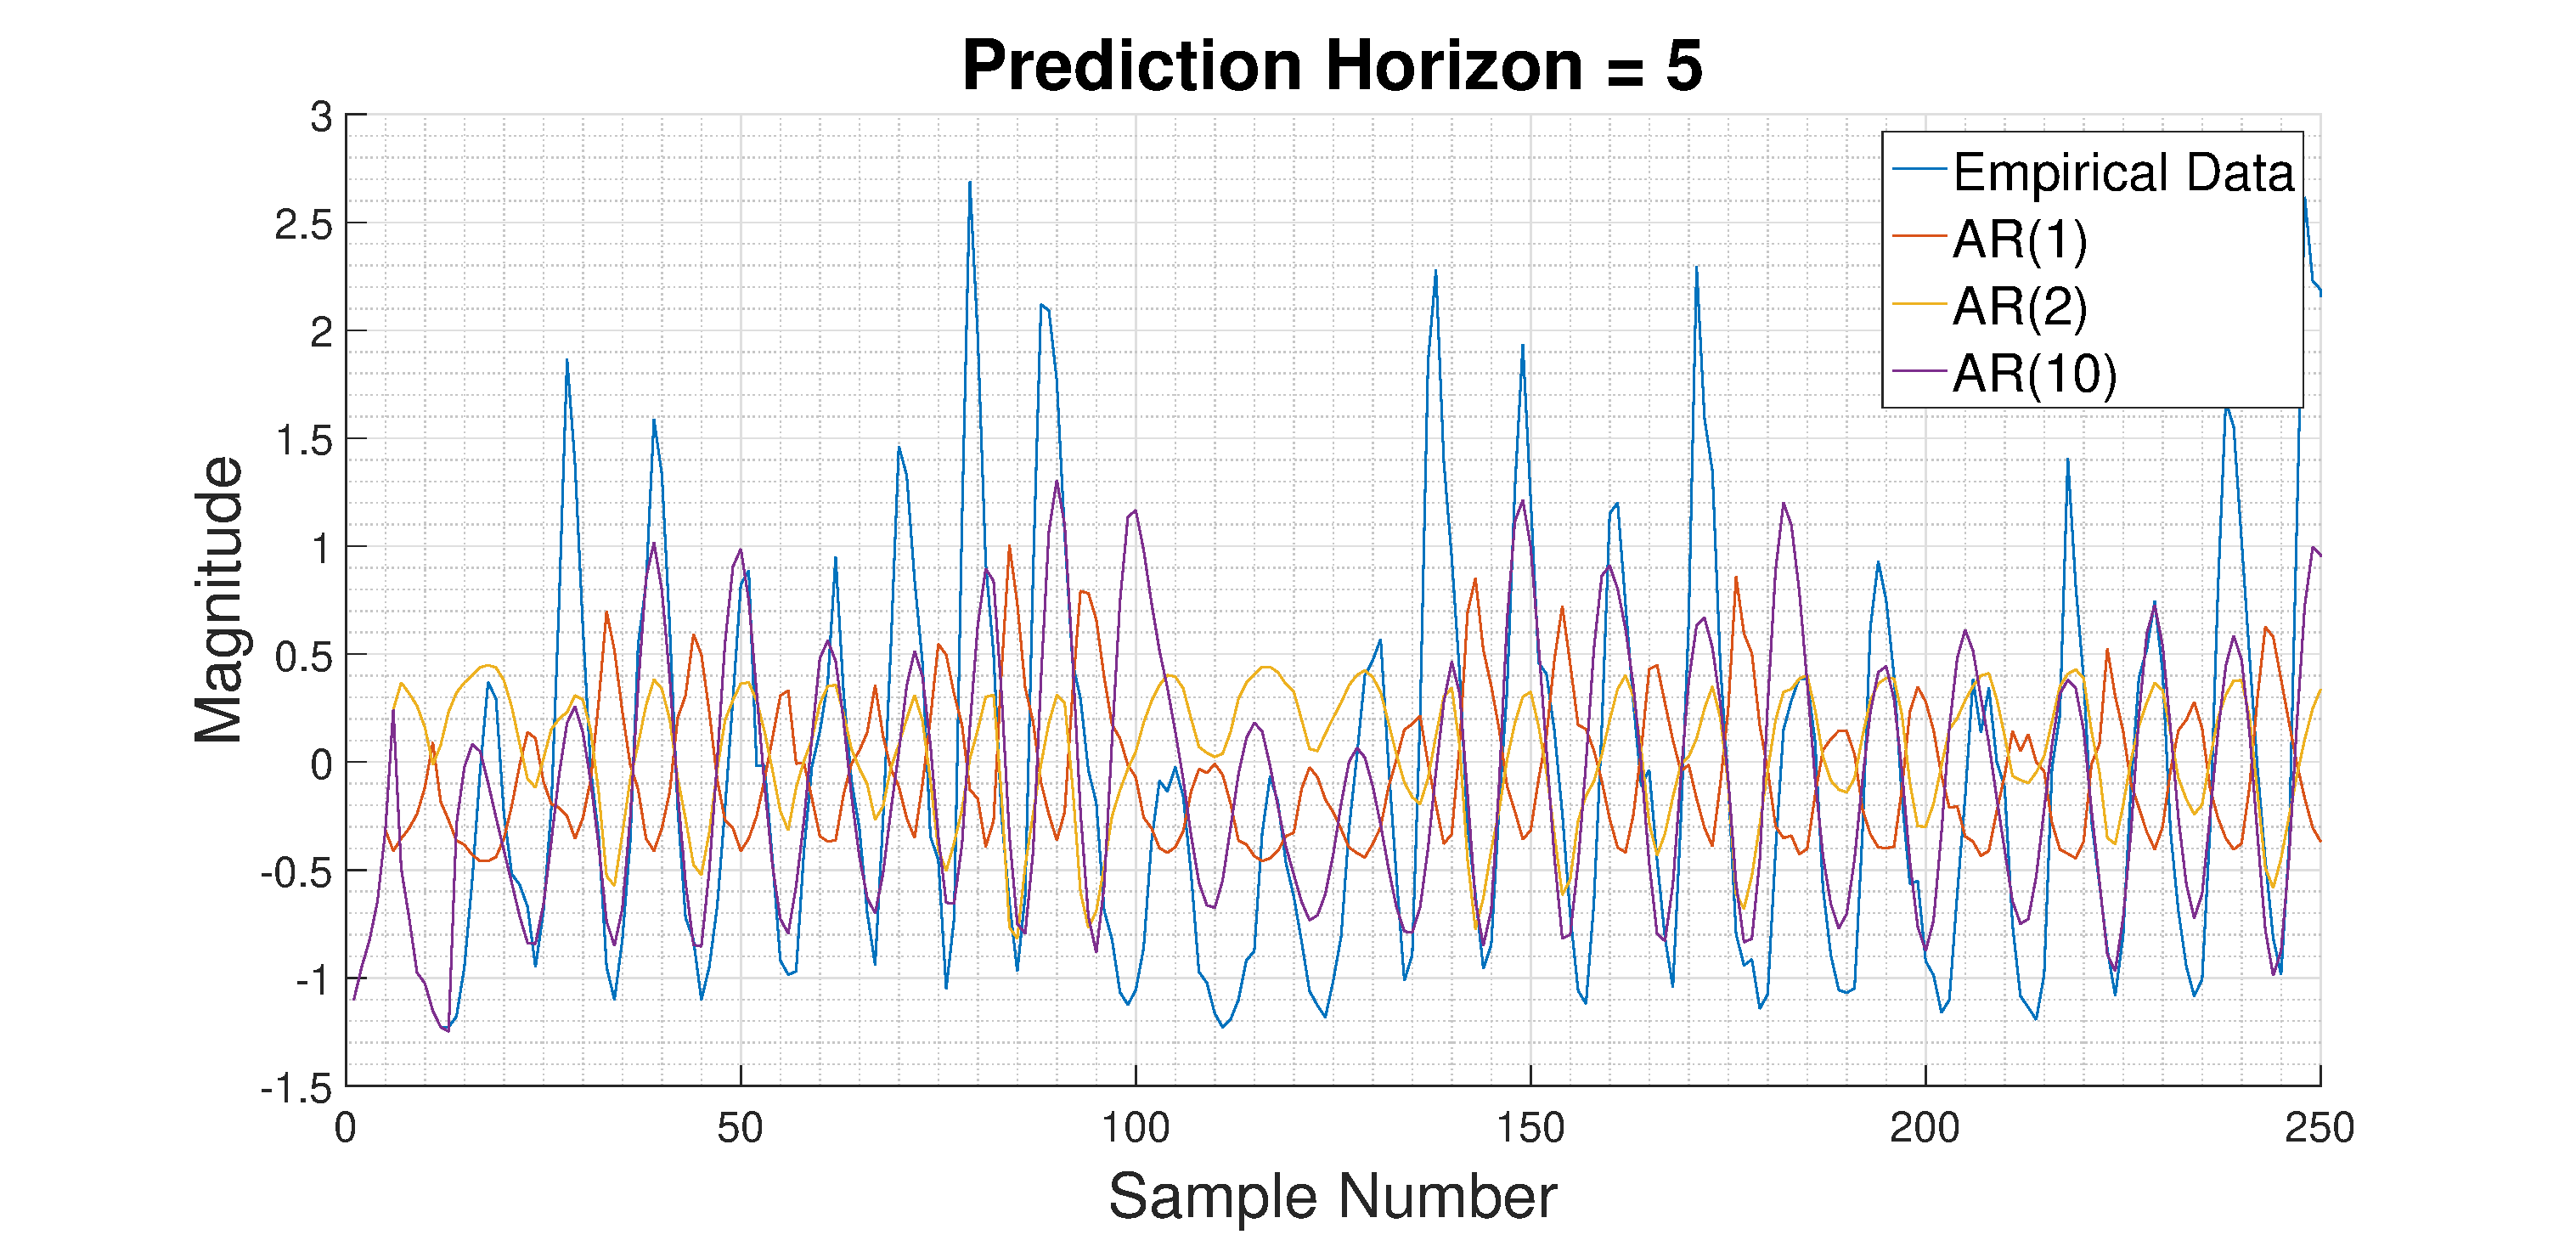
\includegraphics[width = 0.49\textwidth]{sunspot_prediction_horizon_5}
    \caption{Sunspot time series prediction: horizon = 1 and horizon = 5}
    \label{fig:ar_prediction_3}
\end{figure}

\subsection{Real World Signals: ECG from iAmp Experiment}

a) The probability density estimates of the original and averaged heart rate, with $\alpha$=1.0 is graphed in figure \ref{fig:heart_rate_pde_1}. The {\tt pdf} function was utilised to obtain the estimates.

\begin{figure}[H]
    \centering
    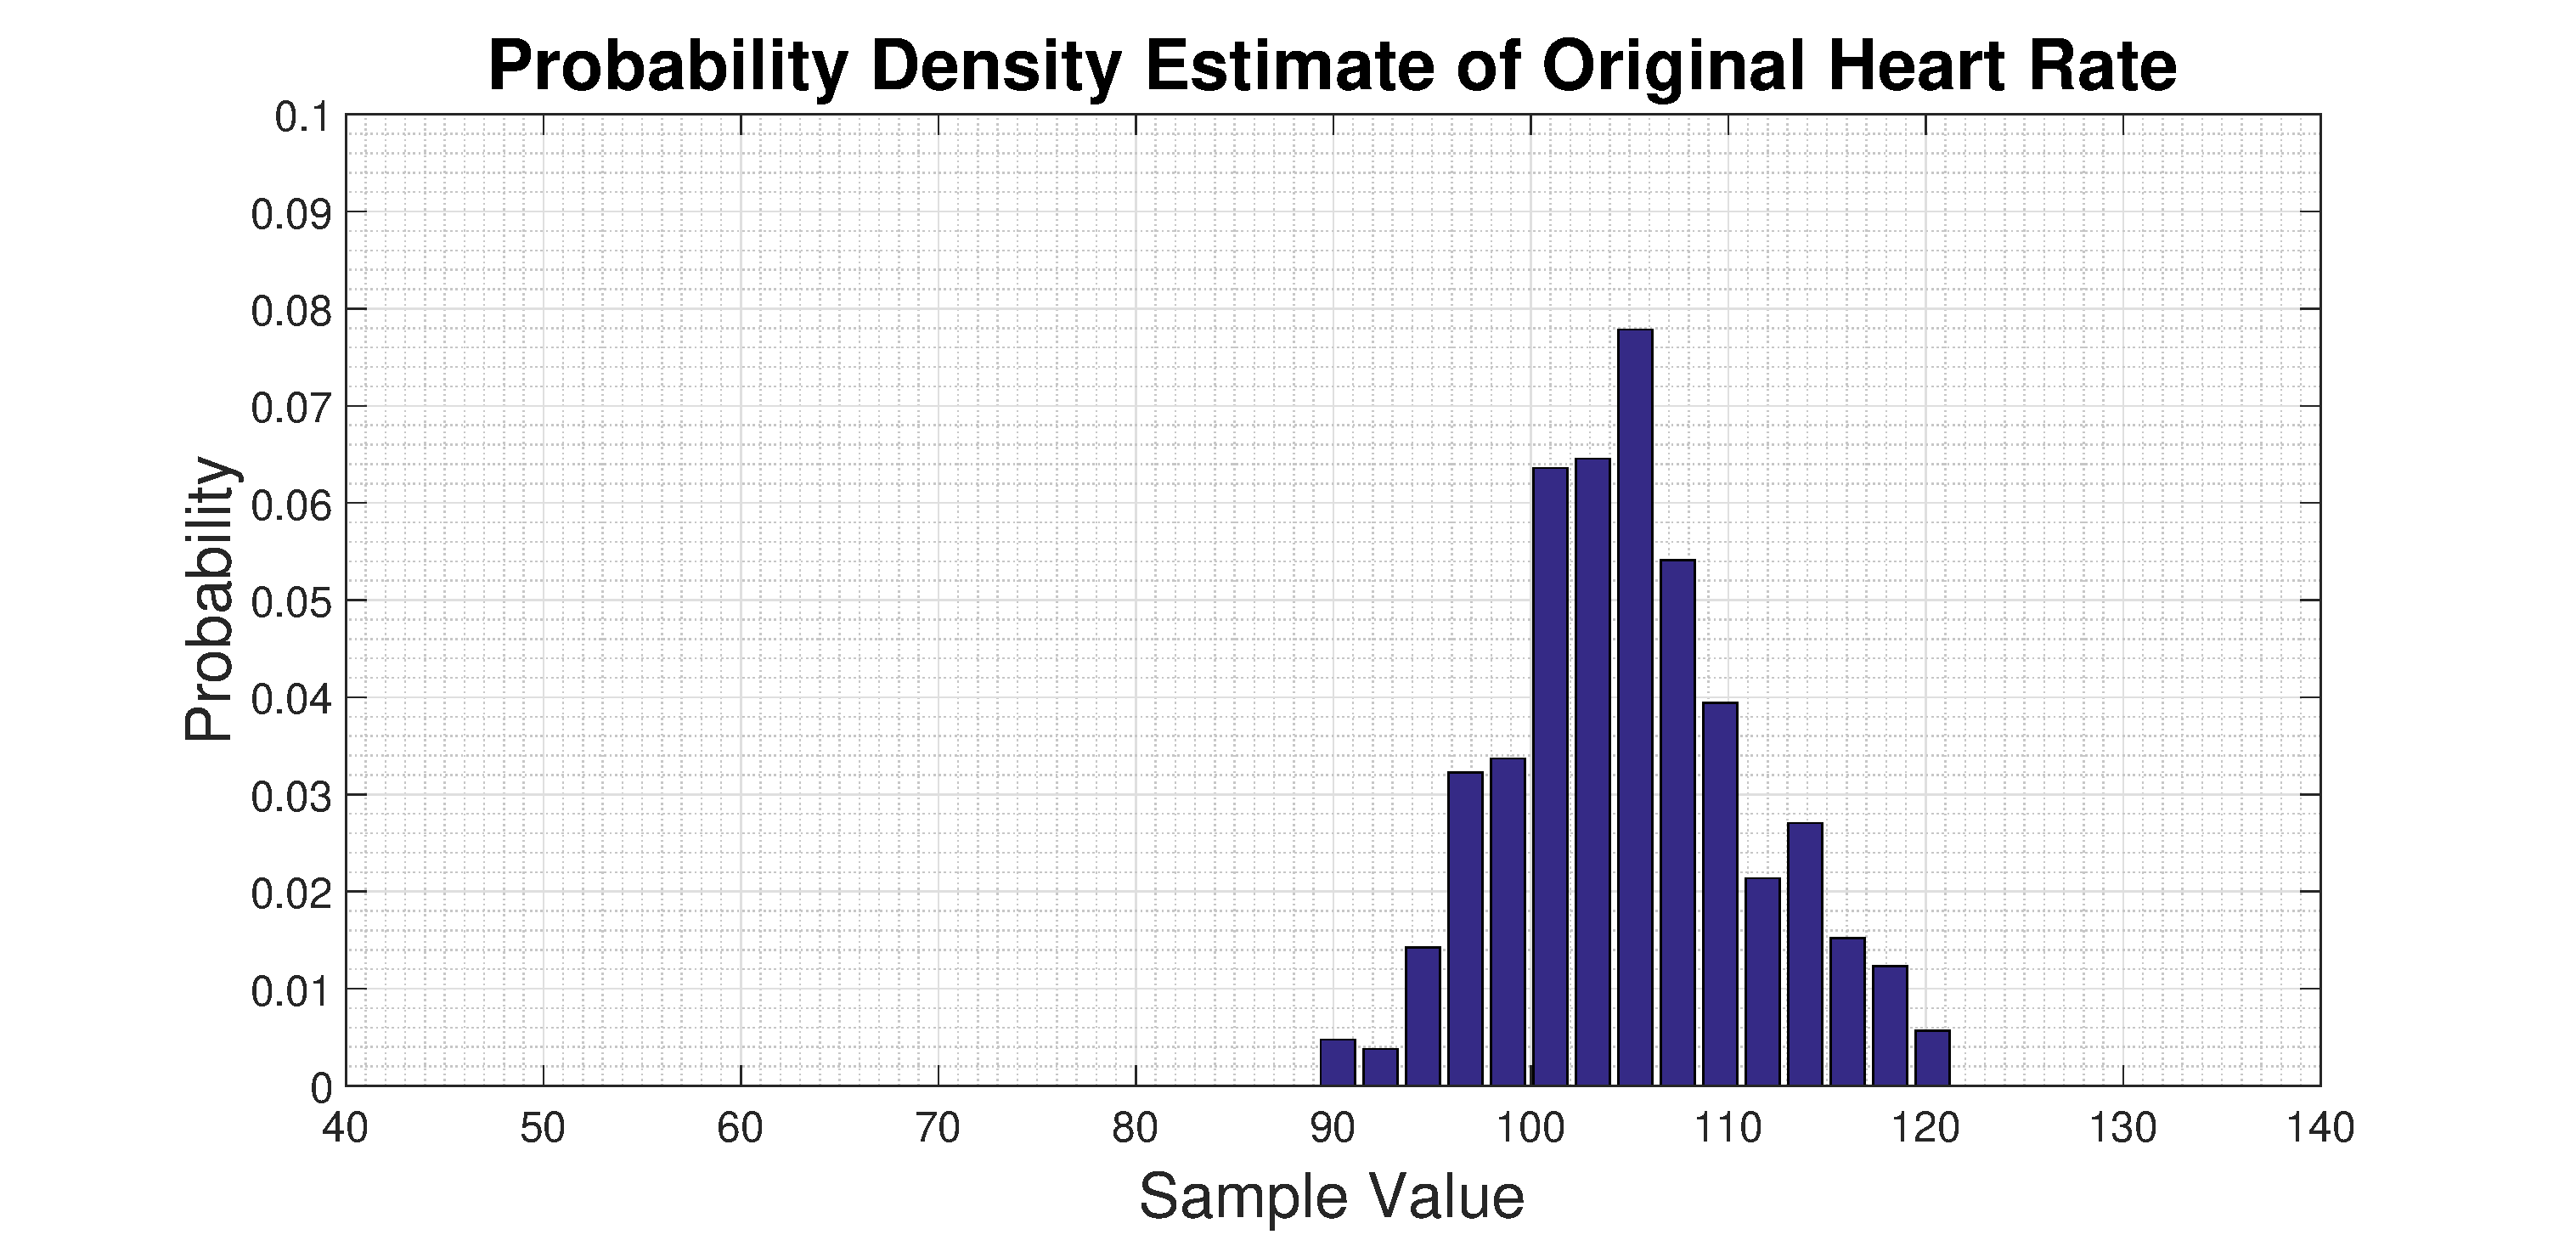
\includegraphics[width = 0.49\textwidth]{pdf_heart_rate_original}
    \includegraphics[width = 0.49\textwidth]{pdf_heart_rate_averaged_alpha_1}
    \caption{Probability density for original heart rat and averaged heart rate, with $\alpha$=1.0}
    \label{fig:heart_rate_pde_1}
\end{figure}

\newpage
The probability density estimates of the averaged heart rate, with $\alpha$=0.6 is graphed in figure \ref{fig:heart_rate_pde_2}.

\begin{figure}[H]
    \centering
    \includegraphics[width = 0.49\textwidth]{pdf_heart_rate_averaged_alpha_point_6}
    \caption{Probability density for averaged heart rate, with $\alpha$=0.6}
    \label{fig:heart_rate_pde_2}
\end{figure}

b) Firstly, it is important to note that the heart rate for each trial has been modelled as a stationary process. As discussed in section \ref{sec:pdf_m}, obtaining the pdf of a non-stationary process using the {\tt pdf.m} is not possible. As such, each sample of the heart rate is 1 realisation of a random variable $H$.\\

The averaging process, as described in equation (15) of the Advanced Signal Processing coursework, will have the effect of reducing the variance of the probability density estimate. The averaged data are no longer unique realisations of the random variable $H$; they are unique realisations of the random variable $\hat{H}$. If the original heart rate, $H$ has a variance of $\sigma_{H}$, averaging every $L$ samples will reduce the variance of the new heart rate, $\hat{H}$, by a factor of $L$, to $\frac{\sigma_{H}}{L}$. This is clearly observed in figure \ref{fig:heart_rate_pde_1}. The original estimate is a lot wider than the averaged estimate.\\

Multiplying by a constant $\alpha$ has two effects. Firstly, it shifts the mean of the estimator. Shifting the mean of the estimator might introduce a bias into the estimate. Alternatively, if the way in which the data was obtained is biased, multiplication by $\alpha$ might be deliberately introduced to remove the bias and obtain an unbiased estimate; in the case of the unbiased estimate of the ACF, a scaling factor of $\frac{1}{N-|\tau|}$ was introduced to remove the inherent bias in the estimate.\\ 

Multiplication by a constant will also have the effect of changing the variance of the estimate. When the variance of a random signal is to be computed, constant terms are taken out of the expectation operator and are squared. Multiplying by $0.6$ will have the effect of reducing the variance to $0.36$ of its original value. The estimate in figure \ref{fig:heart_rate_pde_2} has a variance that is smaller than the averaged estimate in figure \ref{fig:heart_rate_pde_1}. This is exactly as expected.\\

c) Figures \ref{fig:acf_rri_1} and \ref{fig:acf_rri_2} show the ACF for the three RRI time series. The MATLAB function {\tt detrend} has been used to remove linear biases from the data.

\begin{figure}[H]
    \centering
    \includegraphics[width = 0.49\textwidth]{acf_rri_1}
    \includegraphics[width = 0.49\textwidth]{acf_rri_2}
    \caption{ACF for RRI time series: trial 1 and trial 2}
    \label{fig:acf_rri_1}
\end{figure}

\newpage
It is evident that physical process used compute the RRI is autoregressive. The ACF of an MA process is finite in length and goes to 0 after a certain value of $\tau$. The amount of delay after which the ACF goes to 0 represents the order of the MA process; the ACF of MA process has a similar shape to the graph presented in figure \ref{fig:cross_correlated}. The ACF of an AR process is infinite in length. It has a sinusoidal shape. As such, it is clear that the RRI data should be modelled as an AR model rather than a MA process.  

\begin{figure}[H]
    \centering
    \includegraphics[width = 0.49\textwidth]{acf_rri_3}
    \caption{ACF for RRI time series: trial 3}
    \label{fig:acf_rri_2}
\end{figure}


4. The three model selection criteria, namely the MDL, AIC and loss function are graphed for each trial. In addition, the partial correlation function for each trial is graphed as well. The threshold introduced to account for the non-idealities has been reduced from $0.2$ to $0.1$. \\

For trial 1, the model order selection process is rather simple. The data should be modelled as an AR(4) model. Both the MDL and AIC functions have a minimum at 4 and the partial correlation function does not exceed the threshold of $0.1$ after 4.

\begin{figure}[H]
    \centering
    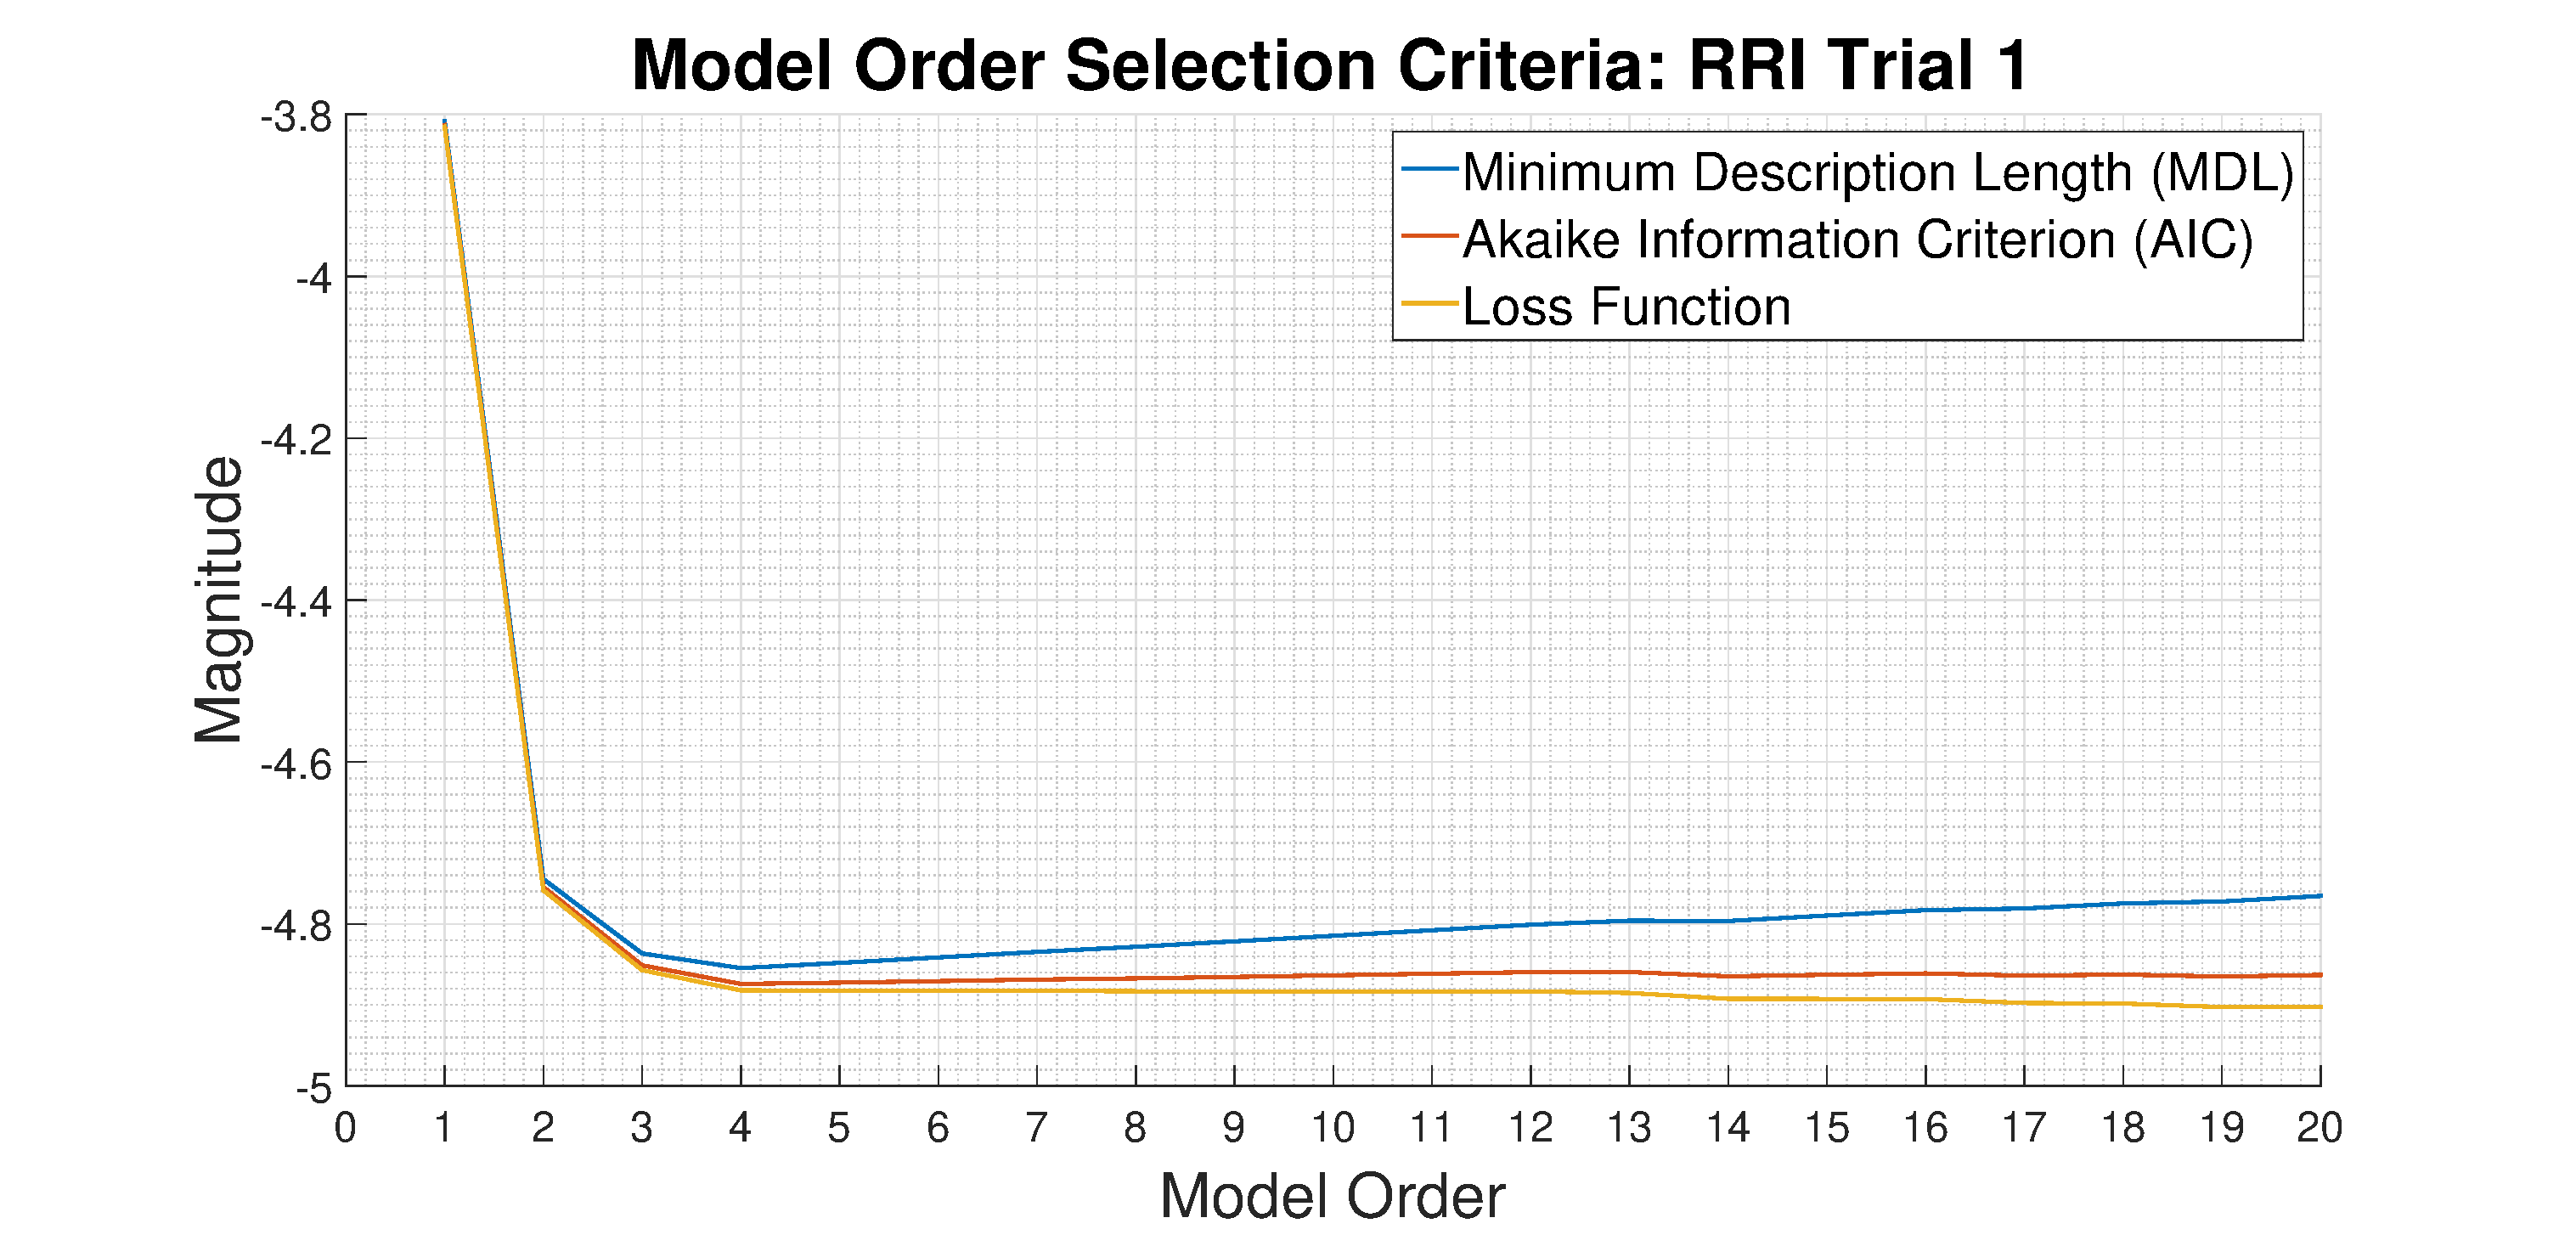
\includegraphics[width = 0.49\textwidth]{MLD_AIC_loss_rri_1}
    \includegraphics[width = 0.49\textwidth]{par_corr_rri_1}
    \caption{Model selection criteria and partial correlation function for RRI Trial 1}
    \label{fig:model_selection_rri_1}
\end{figure}


For trial 2, the model selection process is involved. There a multiple local minima for both the MDL and AIC function. The global minimum of the MDL function occurs at order 16, whereas the global minimum for the AIC function occurs at order 17. For order 17, the partial correlation is below the threshold of $0.1$. As such, trial 2 should be modelled as an AR(16) model. 

\begin{figure}[H]
    \centering
    \includegraphics[width = 0.49\textwidth]{MLD_AIC_loss_rri_2}
    \includegraphics[width = 0.49\textwidth]{par_corr_rri_2}
    \caption{Model selection criteria and partial correlation function for RRI Trial 2}
    \label{fig:model_selection_rri_2}
\end{figure}

\newpage
Similar to trial 1, the model order selection process for trial 3 is straight forward. The data should be modelled as an AR(2) model. Both the MDL and AIC functions have a minimum at 2 and the partial correlation function does not exceed the threshold of $0.1$ after 4.

\begin{figure}[H]
    \centering
    \includegraphics[width = 0.49\textwidth]{MLD_AIC_loss_rri_3}
    \includegraphics[width = 0.49\textwidth]{par_corr_rri_3}
    \caption{Model selection criteria and partial correlation function for RRI Trial 3}
    \label{fig:model_selection_rri_3}
\end{figure}

\newpage
\section{Spectral Estimation and Modelling}

1. Since WGN is a real signal, the PSD of the signal is symmetric about $\pi$. As such, only half of the spectrum is graphed.

\begin{figure}[H]
    \centering
    \includegraphics[width=0.49\textwidth]{pgm_wgn_128}
    \includegraphics[width=0.49\textwidth]{pgm_wgn_256}
    \caption{Periodogram of WGN: $N=128$ and $N=256$}
    \label{fig:pgm_wgn_1}
\end{figure}

The ideal PSD of WGN is unity at all frequencies; the plots in figure \ref{fig:pgm_wgn_1} do not resemble the ideal PSD. A longer sequence consisting of $512$ samples is graphed in figure \ref{fig:pgm_wgn_2}.

\begin{figure}[H]
    \centering
    \includegraphics[width=0.49\textwidth]{pgm_wgn_512}
    \caption{Periodogram of WGN for data length of 512}
    \label{fig:pgm_wgn_2}
\end{figure}

The PSD is evaluated at more unique frequencies since the sequence is longer however the shape is still not ideal. Notice that increasing the number of sample does not cause the estimated PSD to approach the ideal PSD of WGN.\\

Equation (17) from the Advanced Signal Processing coursework can be rearranged to show that the periodogram is actually the Fourier transform of the ACF. The ACF can be calculated through 2 estimators, one that is asymptotically biased while one is asymptotically unbiased. Using the biased estimator, the estimate of PSD may be negative at certain frequencies. To circumvent this, the unbiased estimate of ACF is used. However, as discussed in section \ref{sec:acf_uncorrelated}, the unbiased estimator has large variances at large values of $\tau$. Since every single point in the ACF is used to calculate the PSD estimate, the PSD estimate will also have a large variance. The estimator is inconsistent; the variance of the estimator does not decrease when the number of samples is increased. The bias inherent in the periodogram based estimate of the PSD depends on the window that is applied to obtain a finite length sequence of an infinitely long random process. If a rectangular window is used, the periodogram is asymptotically unbiased.\\

As such, the periodogram based estimates presented in figures \ref{fig:pgm_wgn_1} and \ref{fig:pgm_wgn_2} are asymptotically unbiased but inconsistent; as the number of samples increases, the mean converges to its true value of $1$ however the variance does not converge to $0$.  
\newpage
\subsection{Averaged Periodogram Estimate}

1. Filtering the WGN with a MA filter certainly improves the PSD estimate. The filter smooths out the PSD, removing the large peaks. Mathematically, smoothening the PSD is equivalent to reducing the variance of the estimate. The variance is scaled by a factor which is approximately equal to $\frac{1}{2M+1}$, where $M$ is the order of the MA filter. The decrease in variance comes at a cost; filtering causes the PSD estimate to become biased. Smoothening the PSD also causes the frequency resolution to decrease. By filtering with an MA filter, frequency resolution and estimator bias is traded for reduced variance. 

\begin{figure}[H]
    \centering
    \includegraphics[width=0.49\textwidth]{pgm_filtered_wgn_512}
    \caption{Periodogram of filtered WGN}
    \label{fig:pgm_filtered_wgn}
\end{figure}

2. The 8 periodograms obtained were completely random. The peaks occurred at different frequencies in each estimate. The lack of a distinct pattern in the position of the spectral peaks is attributed to the fact that the ideal spectral is flat and the nonidealities are due to the very large variance rather than a bias at certain frequencies. \\

3. The 8 segments are averaged and the resulting PSD estimate called the averaged periodogram is graphed in figure \ref{fig:pgm_averaged}. An additional graph showing the effects of averaging 64 segments is also shown. Averaging the periodogram certainly reduces the variance in the PSD estimate. The larger the number of segments, the greater the decrease in variance; the decrease is variance is actually $\nicefrac{1}{K}$ where K is the number of segments. 

\begin{figure}[H]
    \centering
    \includegraphics[width=0.49\textwidth]{pgm_averaged_wgn_8_segments}
    \includegraphics[width=0.49\textwidth]{pgm_averaged_wgn_64_segments}
    \caption{Averaged periodogram: 8 and 64 segments}
    \label{fig:pgm_averaged}
\end{figure}

If the length of the sequence is limited, the number of samples in each segment can be reduced; this will lower the frequency resolution of the periodogram. Alternatively, to maintain the same level of frequency resolution, overlapping segments can be used. Overlapping segments may introduce bias into the estimate. As such, obtaining an averaged periodogram is a trade-off between frequency resolution, variance of the estimate and bias of the estimate. 
\newpage
\subsection{Spectrum of Autoregressive Process}

1. Figure \ref{fig:ar_1_periodogram} shows the exact and estimated PSD of the filter defined in the Advanced Signal Processing coursework. The normalised cut-off frequency of the filter is approximately $f=0.3799Hz$. If the PSD estimate is considered as a digital filter itself, it will be a 2\textsuperscript{nd} order filter with a cut-off frequency of $f=0.3555Hz$ 

\begin{figure}[H]
    \centering
    \includegraphics[width=0.49\textwidth]{ar_1_process_estimate_and_ideal}
    \includegraphics[width=0.49\textwidth]{ar_1_process_estimate_and_ideal_zoom}
    \caption{Periodogram of AR(1) process}
    \label{fig:ar_1_periodogram}
\end{figure}

3. The signal used to generate the periodogram is of finite length. Mathematically, a finite length signal is obtained by multiplying the infinitely long signal with a rectangular window. Multiplying by a rectangular window in the time domain is equivalent to convolving the PSD of the signal with a sinc function. The effects of the convolution are not as pronounced at low frequencies because the PSD is almost zero in that frequency range. At high frequencies, the PSD is non-zero and thus the effects of the convolution are obvious.\\

Often the rectangular window is believed to introduces high frequency components into the signal's power spectrum. This is fallacious. Considering the periodogram of the low-pass filter graphed in figure \ref{fig:ar_1_periodogram_2}. It is clear that the effects of the rectangular window will be pronounced in whichever frequency range the PSD is non-zero. 

\begin{figure}[H]
    \centering
    \includegraphics[width=0.49\textwidth]{ar_1_process_estimate_and_ideal_2}
    \includegraphics[width=0.49\textwidth]{ar_1_process_estimate_and_ideal_2_zoom}
    \caption{Periodogram of low pass filter}
    \label{fig:ar_1_periodogram_2}
\end{figure}

4. Periodogram based methods of estimating the PSD do not require a priori knowledge about the way the random samples are generated; these methods do not incorporate knowledge about the type of data. On the other hand, model based estimates take this information into account when generating the estimate. Since the model based estimates are made under the assumptions that the time series follows certain model, if the assumption is correct, the model based estimate should be more accurate than the periodogram based estimate. Figure \ref{fig:model_based_estimate} graphs the model-based estimate of the AR(1) process.

\begin{figure}[H]
    \centering
    \includegraphics[width=0.49\textwidth]{model_based_psd}
    \includegraphics[width=0.49\textwidth]{model_based_psd_zoom}
    \caption{Comparison of model based estimate of PSD to periodogram based estimate of PSD}
    \label{fig:model_based_estimate}
\end{figure}

Equations (20) and (21) from the Advanced Signal Processing coursework are used to estimate the model parameters. Using the equations, $\hat{a}_{1}=0.9128$ and $\hat{\sigma}^{2} = 0.9637$; the estimates are very close to the ideal values of $a_{1}=0.9$ and $\sigma^{2} = 1$. It is clear from figure \ref{fig:model_based_estimate} that the model based estimate is much better than that obtained using the periodogram. This is exactly as expected; the model based estimate of PSD should certainly be closer to the ideal PSD.\\ 

Most notably, the effects of having a finite length sequence rather than an infinitely long sequence manifest by introducing errors in the parameters directly rather than in the PSD estimate; the model-based estimate does not suffer the large errors the periodogram based estimate suffer due to the convolution with the sinc function.\\

5. Figure \ref{fig:sunspot_psd_estimate} shows the PSD estimates of the sunspot time series using both the periodogram and the model-based estimation methods. 

\begin{figure}[H]
    \centering
    \includegraphics[width=0.49\textwidth]{sunspot_psd_estimates}
    \includegraphics[width=0.49\textwidth]{sunspot_psd_estimates_zoom}
    \caption{PSD estimates for sunspot time series}
    \label{fig:sunspot_psd_estimate}
\end{figure}

In section \ref{sec:ar_modelling}, it was concluded that the sunspot time series should be modelled as an AR(2) process. Estimating the PSD using an AR(1) model results in a completely invalid result; the model does not have enough degrees of freedom to represent the periodic nature of the time series. Using an AR(10) model to estimate the PSD, a very large peak is observed. It is clear that the AR(10) model based estimate is closer to the periodogram than the AR(2) model based estimate. However this does not mean that the AR(10) model best represents the data; the periodogram is not the ideal estimate and it suffers multiple shortcomings that have already been discussed. If the model based estimate in figure \ref{fig:model_based_estimate} followed the periodogram exactly, it would be a horrible estimate.\\ 

Moreover, the AR(10) model compresses the power of the time series into a very small frequency range. This suggests that the sunspot series is extremely regular and highly periodic. Looking at \ref{fig:ar_prediction_1}, the effects of modelling the sunspot time series as an AR(10) process are clear. The AR(10) model often pre-empts the existence of peaks. The 2\textsuperscript{nd} order model provides a good balance. The 1\textsuperscript{st} order model severely under models the time series and the 10\textsuperscript{th} order model over models it. 

\newpage
\subsection{Spectrogram for Time-Frequency Analysis: Dial Tone Pad}

1. The signal {\tt y} is graphed in figure \ref{fig:phone_num}. The axis has been adjusted to show the signals generated when the numbers $0$ and $2$ are pressed. 

\begin{figure}[H]
    \centering
    \includegraphics[width=0.49\textwidth]{phone_num}
    \caption{Signal generated when 0 and 2 are pressed}
    \label{fig:phone_num}
\end{figure}

Note that the sampling frequency of $32768$ will allow all frequency components up to the $f=16384Hz$ to be clearly distinguished without aliasing. This will allow the 10\textsuperscript{th} octave to be captured. It is fallacious to think that sampling at such a high rate will increase the frequency resolution. Since we are dividing 1 second of data into 4 non-overlapping segments, the Fast Fourier Transform (FFT) will only be evaluated at frequencies that are multiples of 4.


2. Figure \ref{fig:spectrogram} shows the spectrogram of the signal produced when a random phone number is dialed. The graph is generated using the MATLAB function {\tt spectrogram}; the syntax is {\tt spectrogram(y, hann(8192), 0, 8192, 32768)}. The signal is split into segments of length 8192 with no overlap. Each segment is windowed using the Hanning window. For testing, a seed is used to generate the same random sequence. The phone number that will be used is 0200891960025. 


\begin{figure}[H]
    \centering
    \includegraphics[width=0.49\textwidth,natwidth=610,natheight=642]{spectrogram.png}
    \includegraphics[width=0.49\textwidth]{mag_spec_dial_tone}
    \caption{Spectrogram and magnitude spectrum of dial tone signal}
    \label{fig:spectrogram}
\end{figure}

From the spectrogram, the distinct spectral components of each number are extremely clear. The spectrogram provides the aerial view of the spectrum. The magnitude spectrum provides the side view of the spectrum; the magnitude spectrum for number 1 and number 9 have been graphed. Firstly, the effects of the Hanning window are clear. The ideal spectrum should contain two peaks at two distinct frequencies. The spreading of the spectrum, referred to as spectral leakage, is attributed to the windowing effect. Note that the slight discrepancies in the position of the peaks in the magnitude spectrum are due to the fact that the frequency resolution of the spectrum is poor. As discussed above, the sampling frequency is $32768$ however since each segment is $8192$ samples long, the FFT is only evaluated at 8192 frequencies in the range $[0, $32768$]$. As such, the the peak that should occur at 697 and 1477 occur at 696 and 1448 respectively.\\

3. Each segment of the FFT can be analysed and the two peaks can be located; a threshold should be set, below which the FFT is assumed to not contain any spectral peaks. The spectral peaks can be matched with the frequencies for each number using the table provided in the Advanced Signal Processing coursework.\\

4. Figure \ref{fig:spec_low_noise} shows the time domain signal that has been corrupted by AGWN with $\sigma = 2$. It is interesting to note that the time domain signal is almost nothing like the signal presented in figure \ref{fig:phone_num}. The middle region of the graph, the time in which no number is pressed, is not identifiable. Also note that the signal in figure \ref{fig:phone_num} had an amplitude of 2, whereas the signal in figure \ref{fig:spec_low_noise} has a maximum amplitude of approximately 6. Even though the time domain signal looks nothing like the ideal signal, the spectrogram is still extremely clear. Frequency domain analysis can still be used for key classification.


\begin{figure}[H]
    \centering
    \includegraphics[width=0.49\textwidth]{phone_num_noisy}
    \includegraphics[width=0.49\textwidth,natwidth=610,natheight=642]{spectrogram_low_var.png}
    \caption{Spectrogram and magnitude spectrum of dial tone signal corrupted with low noise}
    \label{fig:spec_low_noise}
\end{figure}

As mentioned, the spectrogram provides the aerial view of the FFT. For the key classification process described above the magnitude spectrum of each segment has to be studied. As such, the magnitude spectra of numbers 1 and 9 are graphed in figure \ref{fig:mag_spec_low_var}. In addition, the magnitude spectrum of a time segment during which no number is dialled is also graphed. 

\begin{figure}[H]
    \centering
    \includegraphics[width=0.49\textwidth]{mag_spec_dial_tone_low_var}
    \caption{Magnitude spectrum of selected FFT segments}
    \label{fig:mag_spec_low_var}
\end{figure}

From \ref{fig:mag_spec_low_var}, it is clear that adding WGN with $\sigma = 2$ does not significantly hinder the key classification process although the time domain signal is almost unrecognizable. Next, noise with $\sigma=8$ is added to the signal. The spectrogram and the FFT of selected segments are graphed in \ref{fig:mag_spec_medium_variance}.


\begin{figure}[H]
    \centering
    \includegraphics[width=0.49\textwidth,natwidth=610,natheight=642]{spectrogram_medium_var.png}
    \includegraphics[width=0.49\textwidth]{mag_spec_dial_tone_medium_var}
    \caption{Spectrogram and magnitude spectrum of dial tone signal corrupted with medium noise}
    \label{fig:mag_spec_medium_variance}
\end{figure}

With the standard deviation of the noise equal to 8, key classification is still possible, however, the threshold set below which the signal is considered to not have any spectral peaks needs to be adjusted. If the threshold is not adjusted, a segment during which a number is not dialled might be interpreted as a segment in which a number is pressed. A smart algorithm can be developed to dynamically determine the value of the threshold based on the input power of the signal. Finally, the spectrogram and FFT of selected segments of a signal that has been corrupted with AGWN with $\sigma=15$ are graphed in figure \ref{fig:spec_large_noise}. The key classification process can no longer be performed because the spectral peaks due to the sinusoidal tones are not distinguishable from the spectral peaks due to the noise. 

\begin{figure}[H]
    \centering
    \includegraphics[width=0.49\textwidth,natwidth=610,natheight=642]{spectrogram_large_var.png}
    \includegraphics[width=0.49\textwidth]{mag_spec_dial_tone_large_var}
    \caption{Spectrogram and magnitude spectrum of dial tone signal corrupted with medium noise}
    \label{fig:spec_large_noise}
\end{figure}

Again the time domain signal produced when medium and large noise were added is graphed in figure \ref{fig:phone_num_medium_and_large_noise}. It is amazing to see that with medium noise, the maximum amplitude of the signal has been increased more than 15 fold; even with this significant increase the key classification process can be conducted with reasonable certainly. Also, note that no sophisticated signal processing has been performed. Neither has a priori knowledge of the signal has been taken into account. This reveals the immense power of analysing signals in the frequency domain. 

\begin{figure}[H]
    \centering
    \includegraphics[width=0.49\textwidth]{phone_num_medium_var}
    \includegraphics[width=0.49\textwidth]{phone_num_large_var}
    \caption{Spectrogram and magnitude spectrum of dial tone signal corrupted with medium noise}
    \label{fig:phone_num_medium_and_large_noise}
\end{figure}

\newpage
\subsection{Real World Signals: Respirator Sinus Arrhythmia from RR-Intervals}

a) Figure \ref{fig:rri_psd_1} shows the estimate of the PSD for the RRI time series using the periodogram method for trial 1 and 2. 

\begin{figure}[H]
    \centering
    \includegraphics[width=0.49\textwidth]{std_periodogram_rri_trial_1}
    \includegraphics[width=0.49\textwidth]{std_periodogram_rri_trial_1}
    \caption{Periodogram based estimate of PSD for RRI time series: trial 1 and trial 2}
    \label{fig:rri_psd_1}
\end{figure}

Figure \ref{fig:rri_psd_2} shows the estimate of the PSD for the RRI time series using the periodogram method for trial 3.

\begin{figure}[H]
    \centering
    \includegraphics[width=0.49\textwidth]{std_periodogram_rri_trial_3}
    \caption{Periodogram based estimate of PSD for RRI time series: trial 3}
    \label{fig:rri_psd_2}
\end{figure}

Next, the averaged periodograms are obtained. The averaging is done by using 5, 150 sample long, segments. Since the FFT would only have been evaluated at 150 unique frequencies, the signal was zero-padded. The averaged periodogram for trial 1 and trial 2 is presented in figure \ref{fig:rri_psd_1_avg}.

\begin{figure}[H]
    \centering
    \includegraphics[width=0.49\textwidth]{avg_periodogram_rri_trial_1_5_segs}
    \includegraphics[width=0.49\textwidth]{avg_periodogram_rri_trial_2_5_segs}
    \caption{Averaged periodogram for RRI time series: trial 1 and trial 2}
    \label{fig:rri_psd_1_avg}
\end{figure}

Lastly, the averaged periodogram for trial 3 is graphed in figure \ref{fig:rri_psd_2_avg}.

\begin{figure}[H]
    \centering
    \includegraphics[width=0.49\textwidth]{avg_periodogram_rri_trial_3_5_segs}
    \caption{Averaged periodogram for RRI time series: trial 3}
    \label{fig:rri_psd_2_avg}
\end{figure}

b) Large spectral components indicate that the test subject's heart rate is high whereas low spectral components indicate the test subject's heart rate is low. Trial 2 and trial 3 provides the RRI data when the test subject was asked to constraint his breathing. It is evident that the pattern of breathing, taking faster shallower breaths, in trial 2 cause the test subject's heart rate to slow down in comparison to the resting heart rate measured in trial 1. The pattern of breathing, taking long deep breaths, in trial 3 cause the test subject's heart rate to increase significantly. 

\newpage
\section{Optimal Filtering - Fixed and Adaptive}
\subsection{Wiener Filter}
1. The signal-to-noise (SNR) ratio for $z[n]$ is equal to $\nicefrac{1}{0.1^{2}} = 100$; in decibels the SNR is $20dB$. Using the statistics $R_{xx}$ and $p_{zx}$, the optimal coefficients calculated are presented in table \ref{tab:wiener_1}.

\begin{table}[H]
  \centering
    \begin{tabular}{|c|c|c|c|c|c|}
        \hline
        \textbf{b} & \textbf{1} & \textbf{2} & \textbf{3} & \textbf{4} & \textbf{5} \\
        \hline
        \textbf{$W_{opt}$ - Empirical Data} & 0.9990 & 1.9995 & 2.9963 & 2.0005 & 0.9973 \\
        \hline
        \textbf{$W_{opt}$ - Normalised Data} & 0.2168 & 0.4367 & 0.6563 & 0.4379 & 0.2155 \\
        \hline
    \end{tabular}%
  \caption{Optimal coefficients of wiener filter}
  \label{tab:wiener_1}%
\end{table}%

The coefficients obtained are extremely close to the ideal values. Using normalised data, the power of the signals $x[n]$ and $\hat{y}[n]$ will be identical. However, when normalised data is used, the coefficients obtained are a scaled version of the original.

\begin{table}[H]
  \centering
    \begin{tabular}{|c|c|c|c|c|c|}
        \hline
        \multirow{2}{*}{\textbf{Noise Variance}} & \multicolumn{5}{c|}{\textbf{b}} \\
    \cline{2-6}          & \textbf{1} & \textbf{2} & \textbf{3} & \textbf{4} & \textbf{5} \\
        \hline
        \textbf{0.2} & 0.9954 & 1.9944 & 2.9924 & 1.0000 & 0.9895 \\
        \hline
        \textbf{0.5} & 0.9927 & 1.9906 & 2.9895 & 1.9996 & 0.9836 \\
        \hline
        \textbf{1} & 0.9896 & 1.9864 & 2.9862 & 1.9992 & 0.9769 \\
        \hline
        \textbf{3} & 0.9820 & 1.9757 & 2.9780 & 1.9982 & 0.9604 \\
        \hline
        \textbf{7} & 0.9724 & 1.9624 & 2.9678 & 1.9969 & 0.9397 \\
        \hline
        \textbf{10} & 0.9670 & 1.9549 &2.9620 & 1.9962 & 0.9280 \\
        \hline
    \end{tabular}%
  \caption{Effects of increasing noise variance on estimated coefficients of wiener filter}
  \label{tab:addlabel}%
\end{table}%

Increasing the noise variance causes the error incurred in the estimation of the coefficients to increase. The coefficients seem to be decreasing in magnitude; this is expected. As noise variance is increased, the signal $z[n]$, which is used as the reference signal in the estimation process starts to look more like white noise and less like the filtered signal $y[n]$. White noise is characterised by samples that are uncorrelated. The unknown system $w[n]$ is a moving average filter and has the effect of introducing dependence into the independent white noise signal. If the reference signal has a large proportion of noise and a low proportion of the correlated outputs from the unknown system, then the identified system, which aims to produce a signal that is statistically similar to $z[n]$, should introduce lesser dependence into the signal $\hat{y}[n]$. By decreasing the magnitude of the variables, less dependence is introduced.\\

The mean-squared-error in the estimated signal $\hat{y}[n]$ is graphed for different values of $N_{w}$ in figure \ref{fig:mse_wiener}. Notice that for $N_{w}>4$, the mean-squared-error does not decrease. This shows that over-modelling the system does not result in a better model. The estimated coefficients are extremely small and have almost no effect in determining the current sample. 

\begin{figure}[H]
    \centering
    \includegraphics[width=0.49\textwidth]{mse_optimal_coeffs}
    \caption{Mean-squared-error in the estimated signal $\hat{y}[n]$}
    \label{fig:mse_wiener}
\end{figure}

3. The number of multiplications and additions can be determined by analysing each step of the algorithm. To estimate the complexity of computing the ACF, the number of multiplications and addition at each value of $\tau$ is considered. Assuming that the data length, N, is significantly large than the number of coefficients, $N_{w}+1$, the number of multiplications at each value of $\tau$ is approximately, N whereas the number of additions is also N. The ACF has to be calculated for $N_{w}+1$ delays. As such, the ACF takes $(N_{w}+1)N$ multiplications and $(N_{w}+1)N$ additions. The cross correlation also takes $(N_{w}+1)N$ multiplications and $(N_{w}+1)N$ additions and the inverting of the matrix takes approximately, $(N_{w}+1)^{3}$ operations.

\subsection{Least Mean Square (LMS) Algorithm}

1. The LMS algorithm is used for system identification. The results obtained after the LMS algorithm has run through the entire data set are presented in table \ref{tab:lms}. The signal $y$ was not normalised to have unity variance; this allows a clearer comparison to the ideal values.

\begin{table}[H]
  \centering
    \begin{tabular}{|c|c|c|c|c|c|c|c|c|c|c|}
    \hline
    \multirow{3}{*}{\textbf{Noise Variance}} & \multicolumn{10}{c|}{\textbf{b}} \\
\cline{2-11}          & \multicolumn{5}{c|}{\textbf{Wiener Solution}} & \multicolumn{5}{c|}{\textbf{LMS Solution, $\mu$ = 0.01}} \\
\cline{2-11}          & \textbf{1} & \textbf{2} & \textbf{3} & \textbf{4} & \textbf{5} & \textbf{1} & \textbf{2} & \textbf{3} & \textbf{4} & \textbf{5} \\
    \hline
    \textbf{0.2}  & 0.9954 & 1.9944 & 2.9924 & 1.0000 & 0.9895 & 0.9942 & 2.0516 & 2.9536 & 2.0113 & 0.9897 \\
    \hline
    \textbf{0.5}& 0.9927 & 1.9906 & 2.9895 & 1.9996 & 0.9836 & 0.9873 & 2.1154 & 2.8954 & 2.0251 & 0.9755 \\
    \hline
    \textbf{1} & 0.9896 & 1.9864 & 2.9862 & 1.9992 & 0.9769 & 0.9824 & 2.1623 & 2.8522 & 2.0363 & 0.9652 \\
    \hline
    \textbf{3} & 0.9820 & 1.9757 & 2.9780 & 1.9982 & 0.9604 & 0.9685 & 2.2814 & 2.7434 & 2.0621 & 0.9401\\
    \hline
    \textbf{7}& 0.9724 & 1.9624 & 2.9678 & 1.9969 & 0.9397 & 0.9517 & 2.4295 & 2.6084 & 2.0958 & 0.9089 \\
    \hline
    \textbf{10}  & 0.9670 & 1.9549 &2.9620 & 1.9962 & 0.9280 & 0.9420 & 2.5126 & 2.5313 & 2.1137 & 0.8903 \\
    \hline
    \end{tabular}%
  \caption{Comparison of wiener solution and solution obtained using LMS alogrithm}
  \label{tab:lms}%
\end{table}%


Both the algorithms have utilised the same amount of information however the estimated coefficients are slightly different. The main short-coming of the Wiener solution is that stationarity was assumed and in real-world applications, stationarity is not always guaranteed. However, in this case, the signal $z$ is stationary and thus the wiener solution is expected to be closer to the ideal solution that the LMS algorithm. Moreover, the LMS algorithm does not have the luxury of processing all the data at once; it processes data with a moving window and thus the results obtained are expected to be less accurate. This is observed in table \ref{tab:lms}. For every value of noise variance, the LMS solution produces a worse answer than the Wiener solution. \\

2. The LMS algorithm is used to estimate the signal $\hat{y}[n]$. The output using the LMS is graphed in figure \ref{fig:lms} for two values of the adaptive gain, $\mu$. For small sample numbers, the error signal is both scenarios is large; as the number of samples increases and the amount of information on which the estimated signal is generated increases, the error decreases. The adaptive gain $\mu$ is an extremely important parameter in the LMS algorithm. Observing the results obtained using $\mu = 0.1$, it is clear that the error signal settles to around 0 by the 50\textsuperscript{th} sample. The error signal obtained using $\mu = 0.01$ settles to around 0 at approximately the 300\textsuperscript{th} sample. Although using a smaller value of $\mu$ translates to slower convergence, the estimated signal is bounded. Notice that using $\mu = 0.1$, a very large overshoot appears in the estimated signal; in many applications, such overshoots can cause complete failure and thus a large value of $\mu$ is not always preferred. Note that if the value of $\mu$ is large, convergence is not guaranteed.

\begin{figure}[H]
    \centering
    \includegraphics[width=0.49\textwidth]{lms_mu_point_1}
    \includegraphics[width=0.49\textwidth]{lms_mu_point_01}
    \caption{System identification using LMS algorithm}
    \label{fig:lms}
\end{figure}

\newpage
Next, the evolution of the coefficients is analysed for $4$ distinct values of $\mu$. The results obtained for $\mu = 0.002$ and $\mu = 0.01$ are graphed in figure \ref{fig:coefs_evol_1}.

\begin{figure}[H]
    \centering
    \includegraphics[width=0.49\textwidth]{evol_coefs_mu_point_002}
    \includegraphics[width=0.49\textwidth]{evol_coefs_mu_point_01}
    \caption{Evolution of coefficients for small $\mu$}
    \label{fig:coefs_evol_1}
\end{figure}

For small values of $\mu$ the coefficients gradually approach their asymptotic values. The gradual approach towards the asymptotic values accounts for the lack of an overshoot. Notice that very small values of $\mu$ will cause the convergence to be extremely slow. The results obtained for $\mu = 0.1$ and $\mu = 0.4$ are graphed in figure \ref{fig:coefs_evol_2}.

\begin{figure}[H]
    \centering
    \includegraphics[width=0.49\textwidth]{evol_coefs_mu_point_1}
    \includegraphics[width=0.49\textwidth]{evol_coefs_mu_point_4}
    \caption{Evolution of coefficients for small $\mu$}
    \label{fig:coefs_evol_2}
\end{figure}

For $\mu=0.1$, the approach towards the asymptotic values is not gradual. The large adaptive step size causes the coefficients to overshoot from their ideal values. The overshoot in the coefficients translates into an overshoot in the estimated signal as observed in figure \ref{fig:lms}. However, notice that the coefficients converge by the 100\textsuperscript{th} sample. The rate of convergence is extremely fast. Arbitrarily increasing the step size does not result in increased convergence. Notice when $\mu = 0.4$, the coefficients do not converge.

\newpage
\subsection{Gear Shifting}
Gear shifting enables the algorithm to change its learning rate, $\mu$ based on certain parameters. The gear shifting algorithm that is experimented with is presented in equation (\ref{eq:gear_shifting}). The algorithm was first suggested by Matthews \& Xie \cite{matt}. The learning rate is increased when the power of the input signal increases. This is a valid proposition because having increased input power means that the signal's amplitude has increasing. If the learning rate is increased, the estimate is likely to follow the rise in amplitude. Next, the learning rate also depends on the value of the error incurred. Again this is wise; a large error requires a large correction whereas a small error requires a small correction. The learning rate will adapt to the error incurred. 

\begin{align}
    \mu(n+1) = \mu(n) + \rho e(n)\textbf{x}^{T}(n)e(n-1)\textbf{x}(n-1)\label{eq:gear_shifting}
\end{align}


Figure \ref{fig:gear_shifting} is used to compare the two algorithms based on their rise time. 

\begin{figure}[H]
    \centering
    \includegraphics[width=0.49\textwidth]{basic_lms}
    \includegraphics[width=0.49\textwidth]{gear_shifting}
    \caption{Comparison of gear shifting algorithm to basic LMS algorithm}
    \label{fig:gear_shifting}
\end{figure}

It is clear that the improvement is not very significant. In section \ref{sec:vinyl_denoising}, another gear-shifting algorithm called the Normalised LMS will be discussed. The improvement observed in normalised LMS is significant. 

\newpage
\subsection{Identification of AR Process}\label{sec:ar_identify}
1. Using the LMS algorithm, the coefficients of the AR(2) process are estimated. The results obtained for small values of $\mu$ are graphed in figure \ref{fig:lms_ar_identification_1}. 

\begin{figure}[H]
    \centering
    \includegraphics[width=0.49\textwidth]{lms_ar_identification_mu_point_001}
    \includegraphics[width=0.49\textwidth]{lms_ar_identification_mu_point_01}
    \caption{Identification of AR(2) process using the LMS: small values of $\mu$}
    \label{fig:lms_ar_identification_1}
\end{figure}

Although the rate of converse is slow, the function works well and is correctly identifying the model parameters. In figure \ref{fig:lms_ar_identification_2}, the results for large values of $\mu$ are presented. Again the results are exactly as expected; beyond a certain threshold value of $\mu$, the LMS results obtained are not accurate. The system becomes unstable. 

\begin{figure}[H]
    \centering
    \includegraphics[width=0.49\textwidth]{lms_ar_identification_mu_point_05}
    \includegraphics[width=0.49\textwidth]{lms_ar_identification_mu_point_1}
    \caption{Identification of AR(2) process using the LMS: large values of $\mu$}
    \label{fig:lms_ar_identification_2}
\end{figure}

\newpage
\subsection{Dealing With Computational Complexity: Sign Algorithms}

Figure \ref{fig:signed_1} shows how the signed-error and signed-regressor algorithms identify the AR parameters in section \ref{sec:ar_identify}.

\begin{figure}[H]
    \centering
    \includegraphics[width=0.49\textwidth]{signed_error}
    \includegraphics[width=0.49\textwidth]{signed_regressor}
    \caption{Identification of AR(2) process using the signed-error and signed-regressor algorithms}
    \label{fig:signed_1}
\end{figure}

Figure \ref{fig:signed_2} shows how the sign-sign algorithm identifies the AR parameters in section \ref{sec:ar_identify}.

\begin{figure}[H]
    \centering
    \includegraphics[width=0.49\textwidth]{sign_sign}
    \caption{Identification of AR(2) process using the sign-sign algorithm}
    \label{fig:signed_2}
\end{figure}

All the algorithms presented have their pros and cons. The signed-error algorithm seems to converge the fastest out it has the largest variance around the steady state value. Both the signed-regressor and sign-sign algorithms have slower convergence ranges but have smaller steady state error. The signed-regressor and sign-sign algorithms seem almost identical however notice the small difference near sample number 3800. It seems as if the signed-regressor algorithm is poorer at dealing with shocks at steady state as compared to the sign-sign algorithm. 

\newpage
\section{A Real World Case Study: Vinyl Denoising}\label{sec:vinyl_denoising}

1. Listening to both tracks, the ticking sound can be clearly distinguished. The tick is of a very regular nature; it is periodic. Thus it is expected that the noise will appear as a sharp peak in the frequency spectrum. The periodograms of both channels are graphed in figure \ref{fig:s2h_corrupt}. Note that the frequency axis of the periodogram represents normalised digital frequencies. To obtain the equivalent frequency of the analogue signal, the sampling frequency needs to be known. In this case, the signal was sampled at $44.1kHz$. The spectral components corresponding to the ticks cannot be fully distinguished just by considering figure \ref{fig:s2h_corrupt}, however it is highly likely that the ticks are due to the large peaks at $\omega=0.033$.


\begin{figure}[H]
    \centering
    \includegraphics[width=0.49\textwidth]{corrupted_s2h_left}
    \includegraphics[width=0.49\textwidth]{corrupted_s2h_right}
    \caption{Periodogram of corrupted stairway to heaven tracks}
    \label{fig:s2h_corrupt}
\end{figure}

2. The periodogram of the clean signal is graphed in figure \ref{fig:s2h_clean}.

\begin{figure}[H]
    \centering
    \includegraphics[width=0.49\textwidth]{clean_s2h_left}
    \includegraphics[width=0.49\textwidth]{clean_s2h_right}
    \caption{Periodogram of clean stairway to heaven tracks}
    \label{fig:s2h_clean}
\end{figure}

Notice that the axis of the clean and corrupted periodograms are the same. Comparing the periodograms, it is clear that the initial conjecture that the ticks in the signal are due to the large peak at $\omega=0.033$ is confirmed. Both the left and right tracks have a peak at $\omega = 0.033$ whereas the clean signals do not. The right channel has another peak at approximately $\omega = 0.005$. To locate the exact position of the peaks, the difference between the periodogram of the clean signal and the periodogram of the corrupted signal is graphed in figure \ref{fig:s2h_diff}.

\begin{figure}[H]
    \centering
    \includegraphics[width=0.49\textwidth]{noise_s2h_left}
    \includegraphics[width=0.49\textwidth]{noise_s2h_right}
    \caption{Difference between periodograms of clean signals and periodograms of noisy signals}
    \label{fig:s2h_diff}
\end{figure}


By considering the periodograms graphed in figure \ref{fig:s2h_diff}, the exact position of the spectral components causing the ticking sound can be determined. \\


3. To remove the two spectral peaks observed in figure \ref{fig:s2h_diff}, band stop filters needs to be designed. To implement the filtering process, multiple design methodologies were considered. Firstly, a Chebyshev Type 1 bandstop filter was designed using the MATLAB command {\tt cheby1}. The range of frequencies that have to be stopped are $[180, 200]$ and $[1465, 1525]$; the edge frequencies were specified appropriately. The order of the filter was chosen to be $8$; for an 8\textsuperscript{th} order stopband filter to be designed using the MATLAB {\tt cheby1} function, the argument of the MATLAB function corresponding to order has to be specified as $4$. The magnitude response of the filter was not ideal. The noise was not sufficiently attenuated. When the filtered signal was played, the ticking noise was still obvious. Next, a notch filter was considered. The MATLAB function {\tt irrnotch} was utilised however again the desired stopband attenuation could not be obtained.\\ 

Lastly, the MATLAB command {\tt designfilt} was used to design a digital stopband filter. The order of the filter was chosen to be $20$. The butterworth algorithm was used by the {\tt designfilt} function to meet the specifications. The design produced using the {\tt designfilt} function was actually a cascade of 10 2\textsuperscript{nd} order filters. The magnitude response of the 2 filters, designed using {\tt desginfilt}, are shown in figure \ref{fig:stop_band_filters}.

\begin{figure}[H]
    \centering
    \includegraphics[width=0.49\textwidth]{mag_spec_band_stop_1}
    \includegraphics[width=0.49\textwidth]{mag_spec_band_stop_2}
    \caption{Frequency response of stopband filters designed using {\tt designfilt}}
    \label{fig:stop_band_filters}
\end{figure}

The filters were extremely effective at removing the peak at occurred at $1495Hz$; after filtering, no ticks could be heard in the left channel. The peak occurring at $200Hz$ proved harder to remove; after filtering the ticking sound could still be heard however it is greatly attenuated. \\


4. Figure \ref{fig:compare_periodograms} shows the periodogram of the 3 signals. The periodogram has been plotted in terms of decibels rather than in terms of the absolute magnitude. The decibel scale accentuates the differences between the three signals. 

\begin{figure}[H]
    \centering
    \includegraphics[width=0.49\textwidth]{compare_left}
    \includegraphics[width=0.49\textwidth]{compare_right}
    \caption{Periodogram of clean, corrupted and filtered signal}
    \label{fig:compare_periodograms}
\end{figure}

It is clear that the filter is performing its operation. The periodogram of the filtered signal looks very similar to the periodogram of the clean signal; the large red peaks present in the corrupted signal have been removed. Notice that the filter has also attenuated some spectral components that were in the clean signal; this is inevitable, however the spectral components of the clean signal that have been attenuated contribute very little power to the signal and thus attenuating these components does not introduce a great deal of distortion. Lastly, note that the stopband filter that acts in the frequency range $[180, 220]$ has not attenuated the noise as much as the filter that acts in the frequency range $[1465, 1525]$. This is expected as the filter has a much smaller frequency range to act on. 
 

\begin{table}[H]
  \centering
    \begin{tabular}{|c|c|c|}
    \hline
    \multirow{2}[4]{*}{\textbf{Channel}} & \multicolumn{2}{c|}{\textbf{Relative Error Estimate}} \\
\cline{2-3}          & \textbf{Corrupted} & \textbf{Filtered} \\
    \hline
    \textbf{Left} & 0.22754 & 0.00721 \\
    \hline
    \textbf{Right} & 1.32961 & 0.09198 \\
    \hline
    \end{tabular}%
  \caption{Relative Error Before and after Filtering}
  \label{tab:relative_error_s2h}%
\end{table}%

The relative error of the corrupted signal and the filtered estimate with respect to the \textit{ground truth} recording is presented in table \ref{tab:relative_error_s2h}. The filtering has certainly enhanced the quality of the corrupted signal; the relative error is approximately 30 times lower for the left estimate and 15 times lower for the right estimate. It should be noted although the relative error has been significantly reduced, it is often important to identify the source of the error. From figure \ref{fig:compare_periodograms}, it is clear that the error in the corrupted signal is due to the large peaks whereas in the filtered signal, the error incurred is due to the over-attenuation at the stopband frequencies. This explains why the filtered estimate for the right channel has a greater relative error; two stopband filters have been used and thus the error due to over-attenuation is incurred in 2 unique frequency bands.\\

The relative error does not provide information about the difference in phase between the clean and filtered signals. \\

5. The normalised LMS (NLMS) algorithm is used to filter the corrupted stairway to heaven signal. The algorithm has $2$ parameters, $\mu$ and $N_{w}$. The effects of changing both these parameters is studied. In addition, the corrupted stairway to heaven track was filtered using the basic LMS algorithm. The findings are presented in figure \ref{fig:nlms_s2h}. 

\begin{figure}[H]
    \centering
    \includegraphics[width=0.49\textwidth]{nlms_relative_error}
    \includegraphics[width=0.49\textwidth]{lms_relative_error}
    \caption{Relative error analysis for Stairway to Heaven soundtrack for both NLMS and basic LMS algorithms}
    \label{fig:nlms_s2h}
\end{figure}

Firstly, by observing the y-axis of both graphs, it is clear that the NLMS algorithm returns a much lower relative error as compared to the basic LMS algorithm. The value of $\mu$ for which the basic algorithm performs the best is $0.5$; note that even then the performance of the basic LMS algorithm only approaches that of the NLMS, it does not surpass it. Secondly, choosing a value of $\mu = 0.5$ was a matter of trial and error. Slightly increasing the value of $\mu$ beyond $0.5$ will cause the basic LMS to lose its convergence property. In addition, the value of $\mu = 0.5$ does not represent a universal bound below which convergence is guaranteed. Convergence properties of the basic LMS algorithm are dependent on multiple factors, one of which is the input signal. This highlights the most important benefit of the NLMS algorithm. Convergence properties for the NLMS algorithm are a lot more predictable and independent of the input signal.\\

It should be noted that for the LMS algorithm, a high learning rate is preferred for this data set. The noise in the time series is extremely non-stationary; it is highly periodic and thus the PDF of the noise is constantly changing. High learning rates are preferred for signals with highly non-stationary noise. If the noise is stationary, a small learning rate might decrease the overall error in the estimate since it has a lower steady state error.\\

Next, the squared error using the optimal value of $\mu$ for this data set is studied. The model order is set at 20, $\mu_{NLMS} = 1$ and $\mu_{LMS} = 0.5$. Figure \ref{fig:squared_error} shows how the squared error in the estimate varies as a function of time. 


\begin{figure}[H]
    \centering
    \includegraphics[width=0.49\textwidth]{squared_error_comparison}
    \includegraphics[width=0.49\textwidth]{squared_error_comparison_zoom}
    \caption{Analysis of convergence rates for LMS and NLMS algorithms}
    \label{fig:squared_error}
\end{figure}

The graph reveals two things about the LMS and NLMS algorithms. Firstly, it is clear that the LMS algorithm has a much higher steady state error than the NLMS algorithm. The rate at which the ticking happens is high and thus the NLMS algorithm did not have time to settle to a steady state. Secondly, it is clear that the NLMS algorithm has a much higher rate of convergence than the LMS algorithm. This is expected since the learning rate of the NLMS is adaptive. When the input power is high, the learning rate increases and the overshoot in the estimate is reduced.\\

Both graphs shown in figure \ref{fig:nlms_s2h} indicate that increasing the model order will decrease the error incurred in the estimate. This was discussed in section \ref{sec:ar_modelling} as well. The MDL and AIC models are necessary to put an upper bound on the model order; the model selection criterion place a penalty that quantifies the computational complexity involved in increasing the model order. Without considering computational complexity for the time being, even with the model order being set at 20, the ticking sound can still be heard.\\

Figure \ref{fig:nlms_s2h_1} shows the corrupted signal, the filtered estimate and the clean reference signal for a short duration of the soundtrack. Even when the NLMS algorithm is used with an order of 20, the ticks are still not completely attenuated; in fact, the ticks are still quite significant. Note that the value of $\mu$ was set to 1. As observed in figure \ref{fig:nlms_s2h}, the value of $\mu$ does not matter for large model orders.

\begin{figure}[H]
    \centering
    \includegraphics[width=0.49\textwidth]{s2h_time_domain_order_20}
    \caption{Time domain analysis of filtered estimate made with model order 20}
    \label{fig:nlms_s2h_1}
\end{figure}

To improve the quality of the sound such that a similar performance to that obtained by utilising stopband filters is achieved, the model order is set to $100$. Once again the time domain signal is analysed. The stark improvement in the quality of the signal is clear; the clean signal graphed in blue almost completely overlaps the green signal. The green peaks that could be observed in figure \ref{fig:nlms_s2h_1} are not present in figure \ref{fig:nlms_s2h_2}.

\begin{figure}[H]
    \centering
    \includegraphics[width=0.49\textwidth]{s2h_time_domain_order_100}
    \caption{Time domain analysis of filtered estimate made with model order 100}
    \label{fig:nlms_s2h_2}
\end{figure}

Estimates made using model order 20 and model order 100 are compared in the frequency domain. The graphs are presented in figure \ref{fig:s2h_freq_domain}. As seen in the time domain, the periodogram of the estimate produced using a model order of 20 does not match the periodogram of the clean signal; using a model order of 100, a much better estimate is produced. It is important to note that the NLMS filter is not indiscriminate in the frequencies that it removes from the corrupted signal. Unlike the stopband filters, the NLMS filter does not over-attenuate at the frequencies which contain noise. 


\begin{figure}[H]
    \centering
    \includegraphics[width=0.49\textwidth]{s2h_freq_domain_order_20}
    \includegraphics[width=0.49\textwidth]{s2h_freq_domain_order_100}
    \caption{Frequency domain analysis of Stairway to Heaven soundtrack}
    \label{fig:s2h_freq_domain}
\end{figure}


6. Firstly, before the LMS and NLMS algorithms are used to filter the Liquid Tension Experiment soundtrack, its periodogram is graphed in figure \ref{fig:lte_periodogram}. Again, to accentuate the ticking noise a decibel scale is used.

\begin{figure}[H]
    \centering
    \includegraphics[width=0.49\textwidth]{lte_periodogram_left}
    \includegraphics[width=0.49\textwidth]{lte_periodogram_right}
    \caption{Periodogram of clean and corrupted Liquid Tension Experiment soundtrack}
    \label{fig:lte_periodogram}
\end{figure}

Notice that the corrupted Liquid Tension Experiment soundtrack has spectral peaks at the same frequency as the corrupted Stairway to Heaven soundtrack. However, the periodogram of the clean Liquid Tension Experiment soundtrack has significant spectral components at the frequencies at which the noise occurs. As such, using an indiscriminate filter such as the stopband filters designed above would cause the sound to be distorted. As discussed above, the NLMS algorithm does not over-attenuate the noise and thus it is a much better filter to use for such applications.\\


Similar analysis to that performed in section 5.5 is performed below. The relative error incurred using both the NLMS and the LMS algorithm is studied. The results obtained are graphed in figure \ref{fig:relative_error_lte}.

\begin{figure}[H]
    \centering
    \includegraphics[width=0.49\textwidth]{lte_nlms_relative_error}
    \includegraphics[width=0.49\textwidth]{lte_lms_relative_error}
    \caption{Relative error analysis for Liquid Tension Experiment soundtrack for both NLMS and basic LMS algorithms}
    \label{fig:relative_error_lte}
\end{figure}

The first point to note is that the LMS algorithm was only stable up to a learning rate of $\mu = 0.1$. This is in contrast to the $0.5$ value that was obtained for the Stairway to Heaven soundtrack. The discrepancy corroborates the assertion made that the stability of the LMS algorithm is heavily dependent on the input signal that is used.\\

Once again it is clear that the NLMS algorithm out performs the LMS algorithm in terms of the error incurred. Next, by observing the errors obtained using the NLMS algorithm, patterns start to emerge. Firstly, having a learning rate of higher than $1$ causes the error incurred to increase. Secondly, decreasing the learning rate such that $\mu < 1$ typically decreases the error incurred. The learning rate controls how fast the algorithms corrects its output. As mentioned above, large learning rates are ideal for signals that are highly non-stationary. This ensures that the coefficients of the model converge to the ideal value before the ideal value changes. Low learning rates typically trade the rate of convergence for a decrease in the steady state error. The optimal learning rate for the NLMS and LMS algorithms differs. This is expected because the NLMS algorithm can afford to have a smaller initial learning rate and still converge faster than the LMS algorithm.\\

The periodograms obtained by filtering using the NLMS algorithm with model order equal to 20 and model order equal to 100 are presented in figure \ref{fig:lte_freq_model_20}. 

\begin{figure}[H]
    \centering
    \includegraphics[width=0.49\textwidth]{lte_freq_domain_order_20}
    \includegraphics[width=0.49\textwidth]{lte_freq_domain_order_100}
    \caption{Frequency domain analysis of Liquid Tension Experiment soundtrack}
    \label{fig:lte_freq_model_20}
\end{figure}

Unlike in the case of the Stairway to Heaven soundtrack, increasing the model order does not have a significant effect on the periodogram of the Liquid Tension Experiment soundtrack. This is observed not only in the periodogram but also when the filtered sound is played. The ticks are almost indistinguishable when an order 20 filter is used. Increasing the filter order does not have a significant effect in improving sound quality. The Liquid Tension Experiment soundtrack has significant spectral contents at the frequencies at which the noise occurs and thus attenuating the ticks even slightly has a significant impact on the Signal-to-Noise ratio.

\begin{thebibliography}{}
\bibitem{mandic} 
D. P. Mandic and J. A. Chambers, "On stability of relaxive systems described by polynomials with time-variant coefficients," in IEEE Transactions on Circuits and Systems I: Fundamental Theory and Applications, vol. 47, no. 10, pp. 1534-1537, Oct 2000.
\bibitem{matt}
V. J. Mathews and Z. Xie, "A stochastic gradient adaptive filter with gradient adaptive step size," in IEEE Transactions on Signal Processing, vol. 41, no. 6, pp. 2075-2087, Jun 1993.
\end{thebibliography}

\end{document}
